
% IMPORTANT: This document (probably) needs to be compiled with LuaLaTeX. In
% case you're still not using LuaLaTeX in <insert current year>.

% Choose which document to output
% 0: print
% 1: electronic
\newcommand{\mode}{1}

\ifnum\mode=0
\newcommand{\outformat}{print}
\else
\newcommand{\outformat}{electronic}
\fi
\documentclass[b5paper, 10pt, twoside]{book}

\frenchspacing

% Programming tools
\usepackage{ifthen}     % conditional commands
\usepackage{etoolbox}   % tools for intefacing with internals

\ifthenelse{\equal{\outformat}{print}}{
\newcommand{\innersize}{55.4pt}
\newcommand{\outersize}{110.8pt}
}{
\newcommand{\innersize}{83.1pt}
\newcommand{\outersize}{83.1pt}
}

\newcommand{\topsize}{55.4pt}
\newcommand{\bottomsize}{115.2pt}

% Page layout
\usepackage[
    inner = \innersize,
    outer = \outersize,
    top = \topsize,
    bottom = \bottomsize]{geometry} % modify page layout

% Debugging
%\usepackage{showframe}     % show the page layout grid
%\usepackage{kantlipsum}    % English placeholder text

% Mathematics
\usepackage{amsmath}    % various math macros
\usepackage{mathtools}  % more math
%\usepackage{amsthm}    % theorem/definition/etc. enivornments
\usepackage{amssymb}    % more math symbols
\usepackage{slashed}    % slashed symbols

% Miscellaneous symbols
\usepackage{gensymb}    % adds degree symbol (and other stuff)
\usepackage{ccicons}    % creative commons icons
\usepackage{textgreek}  % macros for greek letters in text

% General styling
\usepackage{emptypage}  % suppress page numbers on empty pages
\usepackage{fancyhdr}   % fancy header designs
\usepackage{titlesec}   % modify appearance of section titles
\usepackage{titletoc}   % customize table of contents

\usepackage{graphicx}   % better graphics

% Text formatting
%\usepackage{setspace}                   % options for line spacing
\usepackage[xspace]{ellipsis}           % fixes spacing around ellipses
\usepackage[letterspace=70]{microtype}  % microtypographic features

% Localization
\usepackage[english]{babel}

% Float customization
\usepackage[
    format = plain, labelfont = bf
]{caption}                  % customize caption formatting
\usepackage{multirow}       % rows spanning multiple columns for tables
\usepackage{tabularray}     % tables using latex3
\usepackage{threeparttable} % tables with notes
\usepackage{tabularx}       % adjust table column widths
\usepackage{booktabs}       % more professional tables

% Vector graphics
\usepackage{pgf}            % backend for tikz and others
\usepackage{tikz}           % generate graphics programmatically
\usepackage{pgfplots}       % plots using pgf
\usepackage{tikz-3dplot}    % easier 3d plots in tikz
%\usepackage{tikz-feynman}  % easy fenyman diagrams

% Font/text backend stuff
%\usepackage[utf8]{inputenc}                % input encodings (no longer needed)
\usepackage[T1]{fontenc}                    % font encodings
\usepackage{fontspec}                       % interface for opentype fonts
\usepackage[bold-style=ISO]{unicode-math}   % fontspec equivalent for math fonts

% Colors
\usepackage{xcolor} % facilitates color in documents

% Miscellaneous packages
%\usepackage{marginnote}        % allows margin notes
\usepackage[inline]{enumitem}   % more options for enumerate environment
\usepackage{hyperref}           % in-document hyperlink references
\usepackage{zref-totpages}      % macro for printing total number of pages

% Custom packages
\usepackage{scpcolors}      %  collection of custom colors
\usepackage{journalnames}   %  journal name macros

\definecolor{grey}{gray}{0.3}

% It's hard to make hyperlinks look tasteful.
\newcommand{\typographersred}{scp-red-dark-3}
\newcommand{\linkblue}{scp-blue-dark-3}

\ifthenelse{\equal{\outformat}{electronic}}
{
\newcommand{\linkcolor}{\typographersred}
\newcommand{\citecolor}{\typographersred}
\newcommand{\urlcolor}{\linkblue}
}{
\newcommand{\linkcolor}{black}
\newcommand{\citecolor}{black}
\newcommand{\urlcolor}{black}
}

\hypersetup{
    linktocpage,
    colorlinks = true,
    linkcolor = \linkcolor,
    citecolor = \citecolor,
    urlcolor = \urlcolor}


% Biblatex data model config file. If you find yourself needing new custom 
% fields in your `.bib` file, put them here.
\begin{filecontents*}{biblatex-dm.cfg}
\DeclareDatamodelFields[type=field, datatype=literal]{collaboration}
\DeclareDatamodelEntryfields{collaboration}
\end{filecontents*}

% biblatex setup
%
% `collabauthoryear` is a custom cite/bibstyle. It's basically `authoryear`, but
% but in citations it uses the `collaboration` field instead of author, if
% available, and in the bibliougraphy it prints the `collaboration` field in
% parentheses, if available. The definitions are found in the respective `.cbx`
% and `.bbx` files.
\usepackage[
    backend = biber,
    language = english,
    natbib = true,
    citestyle = collabauthoryear-comp,
    bibstyle = collabauthoryear,
    sorting = nyt,
    giveninits = true,
    minbibnames = 3,
    mincitenames = 1,
    maxbibnames = 3,
    maxcitenames = 3,
    hyperref = true,
    arxiv = abs,
    uniquename = full]{biblatex}

% Bibliography file
\addbibresource{thesis.bib} 

% These are some modifications to bibliography entry styling:
%   - Remove "in:" before journal name.
%   - Use the 3-em dash for repeat authors.
%   - Set spacing between name initials.
%   - Add interword spacing to acronyms.
\renewbibmacro{in:}{}
\renewcommand*\bibnamedash{\rule[0.48ex]{3em}{0.14ex}\space}
\renewcommand*\bibnamedelimi{\hspace{0.125em}}
\renewcommand*{\mkbibacro}[1]{\textls[70]{\textsc{\MakeLowercase{#1}}}}

% Fields to exclude from bibliography
\AtEveryBibitem{\clearfield{url}}
\AtEveryBibitem{\clearfield{issn}}

% Allow line breaks after lower case letters in URLs and DOIs in bibliography.
% The high penalty ensures that this is only allowed in the rare event the
% URL/DOI overflows into the margin.
\setcounter{biburllcpenalty}{9000}

\DeclareFieldFormat{authortype}{\mkbibparens{#1}}
\DeclareFieldFormat{pubtitle}{\textsb{#1}}

% Citation command for citing included publications
\DeclareCiteCommand{\pubcite}[\AtNextCitekey{\defcounter{maxnames}{99}}]
    {\usebibmacro{prenote}}
    {\textbf{\printfield[pubtitle]{title}}\\
        \printnames[][1-]{author}\\
        \printfield{year}\addcomma\addspace
        \printfield{journaltitle}
        \printfield{volume}\addperiod
        \printfield{number}\addcomma\addspace
        \iffieldundef{eid}
            {}
            {\printfield{eid}\addcomma}
        \iffieldundef{pages}
            {}
            {\printfield{pages}\addcomma}
        \printfield[eprint:arxiv]{eprint}\addperiod}
    {\multicitedelim}
    {\usebibmacro{postnote}}

% Special handling of NASA/ADS eprints
\DeclareFieldFormat{eprint:ads}{%
    {\mkbibacro{ADS}\addcolon}\space%
    \href{https://ui.adsabs.harvard.edu/abs/#1/abstract}{%
        \nolinkurl{#1}%
    }%
}%

% Special handling of IERS technical note eprints
\DeclareFieldFormat{eprint:ierstn}{%
    {\mkbibacro{IERS}\addcolon}\space%
    \href{https://www.iers.org/IERS/EN/Publications/TechnicalNotes/tn#1.html}{%
        \iffieldundef{eprinttype}{}{\texttt{tn}}\nolinkurl{#1}%
    }%
}


\usetikzlibrary{decorations.markings}   % decorations
\usetikzlibrary{arrows.meta}            % more arrow styles
\usetikzlibrary{calc}			        % complex coordinate calculations
\usetikzlibrary{positioning}            % don't remember what this does
\usetikzlibrary{3d}						% 3D coordinates
\usetikzlibrary{graphs}					% graph drawing
\usetikzlibrary{shapes.geometric}       % various geometric shapes

\pgfplotsset{compat=newest}         % needed for newest plot features

\usepgfplotslibrary{fillbetween}    % fill between lines
\usepgfplotslibrary{groupplots}     % grids of plots
\usepgfplotslibrary{colormaps}      % additional colormaps
\usepgfplotslibrary{extracolormaps} % even more colormaps (custom library)

% The default tick color in PGFPlots is grey for some reason. Make it black.
\pgfplotsset{every tick/.append style={color=black}}

% Font settings
%
% Note: the fonts used need to be installed on the system. All these fonts 
% should be included in a modern TeXLive distribution. If not, install the 
% fonts f the fonts and run `luaotfload-tool -u` to update the font database.
\setmainfont{STIXTwoText}[BoldFont=Stix Two Text Semibold]
\setsansfont{OpenSans}
\setmonofont{NotoMono}[Scale=0.91]
\setmathfont{StixTwoMath}[StylisticSet=1]

% Semibold fonts
\newfontface\sbstyle{StixTwoText-Semibold}
\newfontface\sbsfstyle{OpenSans-Semibold}

% Some special styles
\newcommand{\titlestyle}{\sbsfstyle}
\newcommand{\annotatestyle}{\sbsfstyle}
\newcommand{\headstyle}{\sbsfstyle}
\newcommand{\subheadstyle}{\sbsfstyle}
\newcommand{\subsubheadstyle}{\sbsfstyle}

% Additional commands for typesetting semibold (sb) and uppercase (uc) text in
% serif and sans serif (sf) style
\newcommand{\textsb}[1]{{\sbstyle #1}}
\newcommand{\textsbsf}[1]{{\sbsfstyle #1}}
\newcommand{\textuc}[1]{\textls[60]{#1}}
\newcommand{\textucsf}[1]{\textls[60]{\textsf{#1}}}

\SetTblrStyle{remark-tag}{font=\itshape}
\SetTblrStyle{remark-sep}{font=\itshape}
\SetTblrStyle{caption-tag}{font=\bfseries}
\SetTblrStyle{caption}{halign=l}

% Redefine vector command to use bold italics
\renewcommand{\vec}[1]{\symbfit{#1}}

% Special typesetting for annotating plots
\newcommand{\plotlineannotation}[1]{{\scriptsize\annotatestyle #1}}

% Definitions for part, chapter, section, subsection styles
\titleformat{\part}[display]
    {\filcenter\huge\bfseries}{Part \thepart}{1pc}{\vspace{1pc}}
\titleformat{\chapter}[hang]
    {\Large\headstyle\filright}{\thechapter}{0.5em}{}[\vspace{4pt}]
\titleformat{\section}[hang]
    {\large\subheadstyle\filright}{\thesection}{0.5em}{}
\titleformat{\subsection}[hang]
    {\subsubheadstyle\filright}{\thesubsection}{0.5em}{}

% Spacing around headings
%\titlespacing*{\part}{0em}{2pc}{0em}
\titlespacing*{\chapter}{0em}{2pc}{*2.5}
\titlespacing*{\section}{0em}{*2.0}{*2.0}
\titlespacing*{\subsection}{0em}{*2.0}{*2.0}

% Table of contents appearance
\contentsmargin{2.55em}
\dottedcontents{section}[3.8em]{}{2.3em}{1pc}
\dottedcontents{subsection}[6.1em]{}{3.2em}{1pc}

% Redefine plain page style to put page numbers on the outer edge in `twoside`
% mode.
\ifthenelse{\equal{\outformat}{print}}{
    \fancypagestyle{plain}{%
        \fancyhf{}%
        \fancyfoot[LE,RO]{\thepage}%
        \renewcommand{\headrulewidth}{0pt}%
    }
    \pagestyle{plain}
}{
    \pagestyle{plain}
}

% Vector differential operators typeset like vectors
\newcommand{\Nabla}{\vec{\nabla}}
\newcommand{\Div}{\Nabla\cdot}
\newcommand{\Curl}{\Nabla\times}

% Derivatives
\newcommand{\tder}[2]{d#1/d#2}
\newcommand{\der}[2]{\frac{d#1}{d#2}}
\newcommand{\dder}[2]{\frac{d^2#1}{d#2^2}}
\newcommand{\ddder}[3]{\frac{d^2#1}{d#2d#3}}
\newcommand{\dern}[3]{\frac{d^{#3}#1}{d#2^{#3}}}
\newcommand{\inder}[2]{\frac{\mathfrak{d}#1}{\mathfrak{d}#2}}

% Partial derivatives
\newcommand{\pder}[2]{\frac{\partial#1}{\partial#2}}
\newcommand{\pdder}[2]{\frac{\partial^2#1}{\partial#2^2}}
\newcommand{\ppder}[3]{\frac{\partial^2#1}{\partial#2\partial#3}}
\newcommand{\pdern}[3]{\frac{\partial^{#3}#1}{\partial#2^{#3}}}
\newcommand{\tpder}[2]{\partial#1/\partial#2}

% Miscellaneous commands
%\newcommand{\bm}[1]{\vec{#1}}
\newcommand{\unitv}[1]{\symbfit{\hat{#1}}}
\newcommand{\difd}{\,d}
\newcommand{\mean}[1]{\left\langle#1\right\rangle}
\newcommand{\tmean}[1]{\langle#1\rangle}
\newcommand{\vblank}{\vspace{1pc}}
\newcommand{\imp}[1]{\textsf{#1}}
\newcommand{\lssc}[1]{\textls[70]{\textsc{#1}}}
\newcommand{\transp}{\mathsf{T}}
\newcommand{\mand}{\quad\text{and}\quad}

% Bra-ket macros
\newcommand{\bra}[1]{\left\langle#1\right|}
\newcommand{\ket}[1]{\left|#1\right\rangle}
\newcommand{\braket}[2]{\left\langle#1\middle|#2\right\rangle}
\newcommand{\brakett}[3]{\left\langle#1\middle|#2\middle|#3\right\rangle}
\newcommand{\redbrakett}[3]{\left\langle#1\middle\|#2\middle\|#3\right\rangle}

% Command for ignoring large blocks of text. Saves your pinky for RSI.
\newcommand{\nothing}[1]{}

% TODO commands
\newcommand{\needcite}{\textcolor{\typographersred}{[citation needed]}}
\newcommand{\cited}[1]{\textcolor{\typographersred}{[#1]}}
\newcommand{\todo}[1][]{%
   \ifthenelse{\equal{#1}{}}
        {\textcolor{\typographersred}{[TODO]}}
        {\textcolor{\typographersred}{[TODO: #1]}}
}

% Some negative spacing commands
\newcommand{\nen}{\hspace{-5pt}}
\newcommand{\nquad}{\hspace{-10pt}}
\newcommand{\nqquad}{\hspace{-20pt}}

% Miscellaneous list of math operators I've collected over the years
\DeclareMathOperator{\im}{im}
\DeclareMathOperator{\diag}{diag}
\DeclareMathOperator{\id}{id}
\DeclareMathOperator{\Aut}{Aut}
\DeclareMathOperator{\lcm}{lcm}
\DeclareMathOperator{\Inn}{Inn}
\DeclareMathOperator{\chara}{char}
\DeclareMathOperator{\sgn}{sgn}
\DeclareMathOperator{\rad}{rad}
\DeclareMathOperator{\Hom}{Hom}
\DeclareMathOperator{\End}{End}
\DeclareMathOperator{\Sym}{Sym}
\DeclareMathOperator{\Ant}{Ant}
\DeclareMathOperator{\Int}{int}
\DeclareMathOperator{\supp}{supp}
\DeclareMathOperator{\rank}{rank}
\DeclareMathOperator{\Lie}{Lie}
\DeclareMathOperator{\tr}{tr}
\DeclareMathOperator{\tdet}{det}
\DeclareMathOperator{\Li}{Li}
\DeclareMathOperator{\Br}{Br}
\DeclareMathOperator{\ceil}{ceil}
\DeclareMathOperator{\arccosh}{arccosh}
\DeclareMathOperator{\arctanh}{arctanh}
\DeclareMathOperator{\erf}{erf}
\DeclareMathOperator{\med}{med}

% Environment for the copyright page
\newenvironment{copyrightpage}{\footnotesize\noindent\ignorespaces}{\thispagestyle{empty}}

\newcommand{\institution}{University of Helsinki}
\newcommand{\faculty}{Faculty of Science}
\newcommand{\department}{Department of Physics}

\newcommand{\defenseplace}{\textcolor{\typographersred}{[place]}}
\newcommand{\defensedate}{March 6, 2025}
\newcommand{\defensetime}{\textcolor{\typographersred}{[time]}}

\newcommand{\thesistitle}{Dark Matter in Next Generation Detectors}
\newcommand{\thesisauthor}{Sebastian Sassi}
\newcommand{\thesisyear}{\the\year}

\newcommand{\hipseriesnumber}{\textcolor{\typographersred}{HIP-\thesisyear-XX}}
\newcommand{\isbnp}{\textcolor{\typographersred}{XXX-XXX-XXX-XXX-XXX}}
\newcommand{\isbne}{\textcolor{\typographersred}{XXX-XXX-XXX-XXX-XXX}}
\newcommand{\issnp}{\textcolor{\typographersred}{XXXX-XXXX}}
\newcommand{\issne}{\textcolor{\typographersred}{XXXX-XXXX}}

% End of general stuff everything below is very specific to my thesis.

\newcommand{\bubblestyle}{dashdotted}
\newcommand{\liquidnoblestyle}{solid}
\newcommand{\semiconductorstyle}{dashed}
\newcommand{\scintcrystalstyle}{densely dotted}

\newcommand{\naifillcolor}{scp-red-light-1}

\newcommand{\naicolor}{scp-red-dark-1}
\newcommand{\cawocolor}{scp-purple-dark-1}
\newcommand{\cfcolor}{scp-green-dark-1}
\newcommand{\xenoncolor}{scp-orange-dark-1}
\newcommand{\argoncolor}{scp-brown-dark-1}
\newcommand{\gecolor}{scp-blue-dark-1}
\newcommand{\sicolor}{scp-grey-dark-1}

\newcommand{\wccolor}{scp-orange-dark-1}
\newcommand{\diamondcolor}{scp-green-dark-1}
\newcommand{\siccolor}{scp-purple-dark-1}
\newcommand{\sapphirecolor}{scp-red-dark-1}
\newcommand{\wcolor}{scp-brown-dark-1}

\newcommand{\nufogcolor}{scp-grey-light-2}

\newcommand{\ppcnocolor}{scp-blue-dark-1}
\newcommand{\lineneutrinocolor}{scp-orange-dark-1}
\newcommand{\hepbcolor}{scp-grey-dark-1}
\newcommand{\atmocolor}{scp-purple-dark-1}
\newcommand{\dsnbreactorcolor}{scp-grey-light-2}

\newcommand{\primarylinecolor}{scp-blue-dark-1}
\newcommand{\secondarylinecolor}{scp-orange-dark-1}

\newcommand{\infernoaxiscolor}{scp-grey-light-3}

\newcommand{\darkmarkcolor}{scp-grey-dark-4}

\newcommand{\plotbgcolor}{scp-grey-light-2!50!white}
\newcommand{\plotfgcolor}{white}

% Words LaTeX doesn't know how to hyphenate
\hyphenation{an-i-so-trop-ic}

\begin{document}

\frontmatter

\begin{titlepage}
    \begin{center}
        \textucsf{HELSINKI INSTITUTE OF PHYSICS} \hfill \textucsf{INTERNAL REPORT SERIES}\\
        \vspace{2.5pc}
        \textucsf{\hipseriesnumber}\\
        \vspace{7.5pc}
        {\titlestyle\Large \thesistitle}\\
        \vspace{2.5pc}
        \thesisauthor\\
        \vspace{7.5pc}
        \department\\
        \institution\\
        Finland\\
        \vspace{7.5pc}
        \textucsf{DOCTORAL DISSERTATION}\\
        \vspace{1pc}
        To be presented for public discussion with the permission of the \faculty{} of the \institution, in \defenseplace{} on \defensedate{}, at \defensetime\\
        \vfill
        Helsinki \thesisyear
    \end{center}
\end{titlepage}

\begin{copyrightpage}
    \thesisauthor\\
    \thesistitle\\
    \institution, \thesisyear, \ztotpages{} pages\\
    Series: Helsinki Institute of Physics, Internal Report Series, \hipseriesnumber\\[\baselineskip]
    \ccbysa\\
    \textcopyright{} \thesisyear{} by \thesisauthor\\
    This work is licensed under \textuc{CC BY-SA} 4.0:\\
    https://creativecommons.org/licenses/by-sa/4.0/\\[\baselineskip]
    Included publications\\
    I \textcopyright{} 2021 by American Physical Society\\
    II \textcopyright{} 2022 by American Physical Society\\
    III \textcopyright{} 2024 by American Physical Society\\[\baselineskip]
    \textuc{ISBN}: \isbnp{} (print)\\
    \textuc{ISBN}: \isbne{} (electronic)\\
    \textuc{ISSN}: \issnp{} (print)\\
    \textuc{ISSN}: \issne{} (electronic)\\
\end{copyrightpage}

\tableofcontents

\chapter{Abstract}

The mystery of the nature of dark matter is one of the great outstanding challenges in modern physics. A large body of observational evidence suggests that the majority of the matter content in the universe is in the form of cold, massive particles, whose nongravitational interactions with ordinary matter are extremely weak. Although the existence of this cold dark matter is strongly supported by observations of its gravitational effects, its properties remain undetermined.

A number of experiments have been built to seek direct evidence of scattering of dark matter with ordinary matter. These experiments use large quantities of various elements and compounds, covered in detector instruments, to maximize the likelihood of observing the exceedingly rare dark matter scattering events. While none of these experiments has yet made a definitive observation of dark matter scattering, over the past two decades they have been highly successful in pushing down the upper limits of the dark matter interaction cross-section with ordinary matter for dark matter masses above one GeV.

Recent advances in low-energy-threshold detector technology have enabled the detection of scattering events with recoil energies down to the order of electron volts. This has made direct detection study of sub-GeV dark matter more viable, where the scattering cross-section has historically been less constrained. At these energy scales, coinciding with the energy scales of atomic binding energies the material physical properties of the detector material become important. This has a number of effects on the signal of scattering events, which need to be accounted for.

This thesis is an investigation of the implications of these material effects on the hypothetical signal of sub-GeV dark matter in next generation detectors. The main effort of this work is a detailed study of the daily modulation of the dark matter signal, induced by an anisotropic response of crystalline detector materials due to the rotational motion of the Earth. The daily modulation signal encodes information about the anisotropy of the dark matter scattering rate, which is traditionally inaccessible to detectors without directional sensitivity. We have therefore studied the prospect of using the daily modulation to aid in distinguishing a dark matter signal from the background of solar neutrinos, which presents an obstacle to the observation sub-GeV dark matter. We have also studied the possibility of using daily modulation to distinguish the presence of an anisotropy in the dark matter velocity distribution. In addition to the daily modulation investigations, this work also includes a molecular dynamics simulation study of defect formation in a number of common and hypothetical detector materials, where we analyze the implications of energy loss in low-energy scattering events on the observed nuclear recoil event rate.

\chapter{Acknowledgements}

% Thank Kimmo and Matti

% Thank collaborators

% Thank the students

%I also acknowledge grants from the Magnus Ehrnrooth foundation, which funded my research during the first, as well as during the third and fourth year of my thesis.

\chapter{Included publications}

This thesis is based on the following publications:
\begin{enumerate}[label = \Roman*, ref = \Roman*]
    \item\label{pub:sassi2021} \pubcite{Sassi2021}
    \item\label{pub:sassi2022} \pubcite{Sassi2022}
    \item\label{pub:sassi2024} \pubcite{Sassi2024}
\end{enumerate}
In publication~\ref{pub:sassi2024} the authors appear in alphabetical order which is conventional in theoretical high energy physics.

\section*{The author's contributions}

For publication~\ref{pub:sassi2021} the author wrote all the numerical code and performed the numerical computations to produce all results shown apart from those shown in figure 3 of the publication. For publication~\ref{pub:sassi2022} the author performed the molecular dynamics simulations for sapphire, silicon carbide, tungsten carbide and tungsten, whereas the simulations for carbon, silicon, and germanium were based on prior data. For publication~\ref{pub:sassi2024} the author wrote all the numerical code and performed the numerical computations for all results, and formulated the decomposition of the transverse Radon transform presented in the publication. The methodology for the likelihood analysis was designed together with the collaborators. All manuscripts were prepared together with collaborators with substantial contributions from the author.

\cleardoublepage
\mainmatter

\chapter{Introduction}

The idea of dark matter has its origins in the observation that not all mass in galactic systems emits light. On one hand, one can observe the orbits of objects within the system, and based on Newton's law of gravitation, estimate of the total gravitational mass of the system. On the other hand, one can observe the light emitted from the system, and estimate the luminous mass of the system. It is not unnatural that these two estimates do not agree exactly. After all, not all mass emits enough light, or light in the correct part of the spectrum, to be detectable by our instruments. However, throughout the 20th century, astronomers began to find great discrepancies between estimates of the luminous and gravitational masses of various astronomical systems. Over time these observations became increasingly difficult to explain with ordinary astrophysical matter. With some additional motivation and evidence from the field of cosmology, this eventually culminated in the consensus that the majority of mass in the universe is in the form of cold dark matter of unknown type, which, despite its large quantity, interacts very little with the ordinary luminous matter, apart from its gravitational attraction.

One of the earliest observations of dark matter is an analysis of the motion of galaxies in the Coma galaxy cluster carried out by \textcite{Zwicky1933}. He demonstrated that the galaxies in the cluster appear to move much faster than implied by the mass estimated from the number of visible galaxies. From this he concluded that the majority of the mass in the cluster must be in the form of dark matter. Later studies of the Virgo cluster by \textcite{Smith1936} and of other systems of galaxies by \textcite{Holmberg1937} gave similar results. The major difficulty posed by these observations was the magnitude of the discrepancy. The observations suggested that the dark matter did not constitute just a significant portion of the mass in these systems, but the vast majority of the mass of the systems.

The second set of pivotal observations in the history of dark matter arrived in the early 1970s in the form of measurements of galactic rotation curves by \textcite{RubinFord1970} and \textcite{Freeman1970}. This far observations on the presence of dark matter had primarily been based on systems of multiple galaxies. However, these studies observed the motions of stars within individual galaxies, and found that the circular speeds of stars in the galaxies appeared to flatten as a function of distance from the galactic center.

The significance of these observations is apparent when one considers their implications on the distribution of mass in galaxies. Using Newtonian gravity, one can calculate that for mass $M(r)$ contained within the radius $r$, the circular speed should be $v_\text{circ}(r)=(GM(r)/r)^{1/2}$. Evidently, if the circular speed remains constant beyond the visible edge of the galaxy, this implies $M(r)\propto r$ near the edge. Therefore, if the observations of rotation curves are correct, the conclusion is either that the distribution of mass continues well beyond the visible boundary of the galaxy, or that Newtonian gravity does not describe the motions of stars correctly.

Neither the observations of galaxy clusters nor of galaxy rotation curves immediately imply anything beyond known physics. Dark matter, as understood by Zwicky, could be any matter that is too faint to observe via optical telescope: clouds of gas, rogue planets, black holes, etc. A subset of such objects which consist of ordinary matter but are not visible to our instruments constitutes the category of massive astrophysical compact halo objects, or MACHOs for short. On the other hand, if we assume that existing theories do not explain the observations, an alternative explanation of the rotation curves to a new type of matter is that Newton's laws do not apply when the acceleration is very small, as is the case for stars far from the galactic center. This hypothesis was originally proposed by \textcite{Milgrom1983} in his theory of modified Newtonian dynamics (MOND). Although MOND was not a complete relativistic theory, various MOND-like theories compatible with general relativity have since been proposed \parencites{Bekenstein2004, Milgrom2009, SkordisZlosnik2021}.

However, in light of the observational evidence available today, the possibilities of a large MACHO contribution to the dark matter content appear limited. MOND-like theories, on the other hand, have difficulties fitting all the observations which are explainable with dark matter. Therefore, today the weight of available observations generally tilts in favor of an unknown species of massive elementary particles---or multiple species of elementary particles---which interact very weakly with ordinary matter, but constitute over 80\% of the matter content of the universe.

Some of the greatest successes in determining the matter content of the universe come from cosmology. Following Einstein's invention of the theory of general relativity, which connected the structure of spacetime to its mass--energy content, \textcites{Friedmann1922, Friedmann1924} and \textcite{Lemaitre1927}---and later \textcites{Robertson1935, Robertson1936a, Robertson1936b} and \textcite{Walker1937}---were able to describe the evolution of spacetime in a homogeneous and isotropic universe filled with matter. This theoretical framework underpins the modern ΛCDM standard model of cosmology, which divides the matter--energy content of the universe into different matter--energy fractions: the dark energy fraction, $\Omega_\Lambda$, the matter fraction, $\Omega_m=\Omega_c+\Omega_b$---consisting of the cold dark matter fraction, $\Omega_c$, and the baryonic (ordinary) matter fraction, $\Omega_b$---and the radiation fraction, $\Omega_r$.

At the same time as the theoretical foundations of cosmology were laid down, observations by \textcites{Slipher1917, Wirtz1922, Wirtz1924, Hubble1929} showed that redshifts of distant galaxies increase with the distance of the galaxies from Earth. In the framework of general relativity, this was readily interpreted as evidence that the universe is expanding. The theory of a homogeneous isotropic universe could be applied to these observations. It enabled scientists to connect the mass--energy content of the universe to the expansion rate, and therefore to the redshift observations, which led to the development of the field of observational cosmology.

The breakthrough in the role of cosmology in measurement of the mass content of the universe is more recent, however, and is to a large part due to the discovery of the cosmic microwave background. The cosmic microwave background radiation is the earliest light in the universe, emitted at the epoch when the universe had cooled down enough for electrons and nuclei to form atoms, allowing light to travel freely. Detected first by \textcite{PenziasWilson1965}, its temperature depends on the local density conditions in the primordial plasma at the time it was emitted, and thus its temperature fluctuations carry a great amount of information about the early expansion history of the universe. Due to the small magnitude of these fluctuations, their measurement had to wait until the 1990s, first by the COBE satellite \parencite{BennettEtAl1996}, and later by the WMAP satellite \parencite{BennettEtAl2013}, and last by Planck satellite. Today, the precision of Planck's instruments has turned the measurement of cosmological parameters into a precision science, which has enabled an accurate determination of the matter content universe, leading to an estimate $\Omega_c/\Omega_b\approx 5.45$ for the ratio of cold dark matter to baryonic matter with an error of around $0.1\%$ \parencite{Planck2018}.

The enormous success of the ΛCDM model goes beyond the Planck data, however. Over the past two decades galaxy surveys such as the Sloan Digital Sky Survey \parencite{SDSSIV2022} and Dark Energy Survey \parencite{DES2018} have made great strides in mapping the distribution of galaxies in the observable universe. These observations can be compared to predictions from ΛCDM to make an independent determination of its parameters, and they find general agreement with the CMB-based measurements \parencite{eBOSS2021}.

A further independent test on ΛCDM comes from the Big Bang nucleosynthesis (BBN)---an epoch in the early universe by which the temperature had fallen low enough for protons and neutrons to bind together and form light nuclei. The BBN determines the abundances of light elements in the universe, and therefore allows for determination of the relevant cosmological parameters from measurements of the present day abundances of light elements. In particular, the BBN is sensitive to the baryon to photon ratio, $n_b/n_\gamma$. Given that the number density of photons, $n_\gamma$, can be determined from the present day CMB temperature, which is known at high precision, the BBN gives an independent estimate of the baryon fraction, $\Omega_b$, which is consistent with the CMB value \parencite{FieldsEtAl2020}. The BBN is furthermore sensitive to the number of relativistic particle species, as well as to the energy input, at the time of BBN, which puts additional constraints on the properties of particles which can contribute to the present day dark matter abundance.

Any model which intends to replace dark matter with modified gravity would have to be able to reproduce both the CMB and galaxy survey observations, but modified theories of gravity including MOND-like behavior historically struggle with reproducing these cosmological observations \parencites{XuWangZhang2015, TanWoodard2018, ZlosnikSkordis2017}. However, it is possible to construct numerous possible extensions of general relativity, which include MOND-like behavior, and there are some claims of success in fitting the observations \parencite{SkordisZlosnik2021}. Therefore, despite the common failure of MOND theories at making cosmological predictions, it remains difficult to completely rule out the hypothesis on a purely cosmological basis.

Besides cosmology, however, a major challenge to MOND-like theories comes from observations of weak gravitational lensing. One of the most important predictions of the theory of general relativity is the bending of light rays as they pass by massive objects due to the effects of mass on the curvature of spacetime. This phenomenon leads to the effect of gravitational lensing, where images of background galaxies become distorted by the gravitational effects of foreground galaxies and clusters. Because the character of the lensing depends on the precise distribution of mass causing the lensing, an image of lensing can, in principle, be used to reconstruct the mass distribution. Modern instrumentation and methods have enabled observations of very weak lensing effects, which in turn has made possible the estimation of distribution of gravitating mass in galaxy clusters.

Some of the most convincing astrophysical evidence for dark matter nowadays comes from weak lensing observations of certain type of galaxy cluster mergers. \textcite{CloweEtAl2006} were the first to present evidence of this nature in their work analyzing the mass distribution of the 1E 0657-56 galaxy cluster---known more commonly as Bullet Cluster---on the basis of weak lensing observations. The Bullet Cluster consists of two concentrations of galaxies, which have two clouds of X-ray emitting plasma between them. This formation suggests that the cluster is the aftermath of a past merger event of two galaxy clusters. In such a merger, the relatively compact galaxies pass each other unimpeded, while the colliding plasma faces a great amount of resistance, slowing it down. This leads to the observed distribution the galaxies and plasma within the cluster.

The plasma contains the majority of the cluster's luminous mass. However, the weak lensing measurements indicate that the total mass of the cluster has two peaks at the locations of the two galaxy subclusters. Under standard assumptions of gravitational interactions these observations imply that the majority of the mass in the Bullet Cluster is dark and collisionless. The observation is therefore evidently in line with the dark matter hypothesis, and it would be difficult to conjure a modified gravity framework that explains this structure and remains consistent with all other observations sensitive to the model of gravitation.

Since the observation of the weak lensing in the Bullet Cluster, observations of numerous similar colliding galaxy clusters have been made. These observations support the hypothesis of collisionless dark matter, and they can be used to place bounds on the self-interaction cross-section of dark matter \parencite{HarveyEtAl2015}.

Although cosmological and astrophysical observations clearly indicate the presence of collisionless dark matter, which constitutes the majority of the mass in the observable universe, they give little information about the nature of this matter. The reason is that the evidence comes from the gravitational effects of dark matter, and as far as gravitation is concerned, anything with mass will do. These observations, therefore, leave open a number of questions about dark matter. How large are the objects that constitute dark matter? Are they macroscopic objects (e.g., MACHOs) or are they microscopic particles? Can they be explained within the Standard Model of particles physics, or do they require new particles and interactions? If dark matter consists of new types of elementary particles, what are their properties?

We may first note that MACHOs that consist of baryonic matter and were created before the BBN are decisively ruled out by the BBN limits on the baryon fraction. Beyond trivial BBN constraints, however, a significant MACHO fraction of dark matter is also heavily constrained by microlensing observations for masses above $10^{-11}$ solar masses \parencite{BirdEtAl2023}. Primordial black holes, in particular, are further constrained by their evaporation via Hawking radiation, which limits their masses to be above roughly $10^{-16}$ solar masses. Therefore, in this mass range there exists only a small window where a significant MACHO dark matter fraction remains viable. This makes MACHOs an unlikely candidate to explain a significant portion of the dark matter content.

In the mid-range of macroscopic dark matter, down to sub-Planck masses, there exists bounds from searches of tracks in ancient mica crystals, which rule out nuclear density dark matter up to around 100 grams, with atomic density dark matter essentially ruled out by cosmology up to the MACHO range \parencite{JacobsStarkmanLynn2015}. Furthermore, large parts of the range for nuclear density dark matter are ruled out by the existence of long-lived white dwarfs, since macroscopic dark matter has the capacity to heat them up \parencite{Graham2018}. In addition, lack of recorded injuries from dark matter collisions also places constraints on this mass region \parencite{SidhuScherrerStarkman2020}.

In practice, these limits suggest that dark matter consists of microscopic particles with masses below the Planck mass. The possibility of exotic composite states of Standard Model particles has been explored in the literature. However, the limited options for constructing models of stable composites, which are created early enough before the BBN, produce sufficient dark matter abundance, and have heavily suppressed interactions, while being consistent with all other observations, leave few plausible candidates---see chapter 9 of the review article of \textcite{CirelliStrumiaZupan2024} for discussion of dark matter in the Standard Model. The theoretical study of dark matter therefore most often considers extensions to the Standard Model of particle physics, which contain new particles whose couplings to the Standard Model particles are in some way suppressed.

In going beyond the Standard Model, we are left with a vast range of possible models of dark matter to explore. Although we can, as discussed above, describe what dark matter probably is not, there is very little to be said about what it is. Assuming that it is a new particle, elementary or composite, we do not know its mass, we do not know its quantum numbers, and we do not know how it couples to the particles of the Standard Model.

A great number of methods and experiments have been devised over the years to find evidence of nonSgravitational interactions of dark matter with ordinary matter. Some of these experiments seek evidence indirectly via observation of a variety of astrophysical signals whose deviation from the expected one---i.e., a signal assuming only Standard Model interactions---would be evidence of the presence of particle dark matter. Other experiments instead look for the most direct evidence: scattering of dark matter particles off ordinary matter in a laboratory setting. Such a direct detection of dark matter, if observed, would be the ultimate evidence for the existence of particle dark matter, as well as the tool for uncovering its properties.

The basic principle of direct detection is deceptively simple: the likelihood of detecting a scattering event in a mass of atoms is directly proportional to the number of atoms. Therefore, you gather as much as atoms as is feasible, and observe them for scattering events. The difficult part, of course, is the practical implementation of such an experiment. One must be able to detect the occurrence of scattering events, and to mitigate against background events from other sources. Despite the associated challenges in implementing direct detection experiments, the last two decades have seen enormous growth in the sizes of these experiments, and consequently, this has led to better bounds on the properties of dark matter.

Direct detection offers an incredible tool for studying the properties of dark matter. On one hand, the study of dark matter scattering with different targets can probe the microphysical interactions between dark matter and ordinary matter. On the other hand, these experiments look for naturally occurring dark matter from our local galactic environment, and can, therefore, in the event of a detection, study the velocity distribution of dark matter, giving further insight into the distribution of dark matter in the Milky Way.

A great challenge for direct detection in the present is directional sensitivity; that is, the ability of experiments to detect the direction of a recoil caused by a scattering event. The ability to sense the direction of scattering events in these experiments would be revolutionary. Due to the motion of the solar system through the galaxy, the Earth experiences a dark matter wind, which leads to an anisotropic angular distribution of scattering events centered on the direction of the wind. This is a unique directional signature which cannot be emulated by any known background. Time projection chambers are the most developed technology for directional detection, and is in active use in some currently operating detectors \parencites{BattatEtAl2017, IkedaEtAl2021}. However, due to the need for low-pressure gases to operate, scaling the technology to match the target masses of existing nondirectional detectors is challenging. Various other methods for detecting particle tracks have been suggested for direct detection, including nuclear emulsions \parencite{AgafonovaEtAl2018}, crystal defects \parencites{RajendranEtAl2017, MarshallEtAl2021}, two-dimensional materials \parencites{CapparelliEtAl2015, MarshallEtAl2021, BaracchiniEtAl2018}, DNA/RNA \parencites{DrukierEtAl2012, OHareEtAl2022}, and paleodetectors \parencite{BaumEtAl2020}. These technologies are in various stages of development and none have yet been implemented at scale.

In the absence of straight directional sensitivity, this thesis explores the limits of presently available direct detection technologies. In particular, this thesis focuses on how the unique material properties of crystalline semiconductor detectors can be exploited to gain information about the directional properties of dark matter scattering without directional sensitivity, and how this information can be used to not only set bounds on the scattering cross-section of dark matter, but can also be used to study the properties of the velocity distribution of dark matter. The regular structure of the crystal lattice gives rise to an anisotropic ionization threshold in semiconductors. In modern low-threshold detectors this is expected to lead to a daily modulation of the direct detection event rate for sub-GeV dark matter due to the rotation of the Earth. 

The contents of the thesis are as follows. Chapter \ref{chap:direct-detection} contains a brief general introduction to the theory direct detection, as well as a discussion of its present status. In publication~\ref{pub:sassi2021} we explored the prospect of using daily modulation for discrimination of a dark matter signal from a background of solar neutrinos. Chapter~\ref{chap:background} gives an introduction to the neutrino background and summarizes the results of publication~\ref{pub:sassi2021}. Chapter~\ref{chap:energy-loss} discusses the properties of crystalline detector materials, including the ionization threshold in semiconductors. Publication~\ref{pub:sassi2024} continued the above program by studying the possibility of discriminating an anisotropic component in the velocity distribution of dark matter using full energy and modulation information. Chapter~\ref{chap:dist} contains a discussion of the dark matter velocity distribution, and offers a detailed discussion of the celestial motions that cause the modulation of the dark matter signal, as well as a discussion on the results of publication~\ref{pub:sassi2024}. Finally, in publication~\ref{pub:sassi2022} we investigated the phenomenon of energy loss to lattice defects due to low-energy recoil events in a number of common and potential detector materials using classical molecular dynamics simulations. Understanding of the phenomenon of energy loss is important for correct interpretation of signals in low-threshold phonon-mediated detectors and also has potential to aid in discrimination of nuclear and electronic recoils \parencite{HeikinheimoEtAl2022}. Chapter~\ref{chap:energy-loss} also contains a discussion of the principles of defect formation and energy loss, and outlines the results of publication~\ref{pub:sassi2022}.

\chapter{Dark matter scattering and direct detection}
\label{chap:direct-detection}

If the elementary particle hypothesis of dark matter is true, then the dark matter particles should occasionally interact with particles of ordinary matter. This interaction is necessarily extremely weak, given the fact that such interactions have never been definitively observed. According to present understanding of distribution of dark matter, the Milky Way sits in the center of a spherical halo of dark matter particles. Under this model of the distribution of dark matter, there should exist a constant stream of dark matter particles traveling through the Earth. Therefore, if the hypothesis is true, given a sufficiently large detector, scattering events between dark matter and the target material of the detector should produce a detectable signal. This is the basic premise that underlies the efforts of direct detection of dark matter.

A theoretical description of direct detection can be given in the framework of scattering theory. Classically, the rate of particles scattering off a particle with cross-section $\sigma$ traveling at velocity $\vec{v}$ with number density $n$ is given by $\sigma vn$. For dark matter particles with velocity distribution $f(\vec{v})$ the total rate of scattering events per unit mass is
\begin{equation}
    R_S=\frac{n_\text{DM}}{m_T}\int\sigma vf(\vec{v})\difd^3v,
\end{equation}
where $N_S$ denotes the total number of scattering events off the target, and $m_T$ is the mass of the target particle. Rather than considering the total scattering rate, it is useful for the analysis to consider the rate of scattering events per unit of momentum transfer per solid angle,
\begin{equation}
    \ddder{R_S}{q}{\Omega}=\frac{n_\text{DM}}{m_T}\int\ddder{\sigma}{q}{\Omega}vf(\vec{v})\difd^3{v}.
\end{equation}
Here $q$ is the magnitude of the momentum transferred to the target, $\vec{q}=\vec{p}-\vec{p}'$, where $\vec{p}$ and $\vec{p}'$ denote the initial and final momenta of the dark matter particle, respectively.

Typical models of dark matter assume that the dark matter in the halo is cold; that is, that it is nonrelativistic. It follows that the scattering of dark matter in direct detection can typically be treated as nonrelativistic. Therefore, the scattering of a dark matter particle with initial momentum $\vec{p}$ and final momentum $\vec{p}'$ off a target can be formulated as a nonrelativistic two-to-two scattering problem from an initial state $\ket{i,\vec{p}}$ to a final state $\ket{f,\vec{p}'}$, where $i$ and $f$ refer to the initial and final states of the target particle. The scattering cross-section is then given by the formula
\begin{equation}
    \ddder{\sigma}{q}{\Omega}=\frac{1}{v}\frac{1}{(2\pi)^3 16m_\text{DM}^2m_T^2}\sum_f2\pi\delta(E_f-E_i-\omega_{\vec{q}})\left|\brakett{f,\vec{p}'}{H_\text{int}}{i,\vec{p}}\right|^2,
\end{equation}
where the summation over the final states in case of continuous momentum states is to be interpreted as integration with the appropriate measure, and $v=|\vec{v}-\vec{v}_T|$ represents the magnitude of the difference of the initial velocities of the particles. The energy deposition $\omega_{\vec{q}}$ is defined as
\begin{equation}
    \omega_{\vec{q}}\equiv E_{\vec{p}}-E_{\vec{p}'}=\vec{q}\cdot\vec{v}-\frac{q^2}{2m_\text{DM}}.
\end{equation}

If the initial and final states of the target can be described as plane waves with momenta $\vec{k}$ and $\vec{k}'$, then the scattering amplitude can be written as
\begin{equation}
    \brakett{\vec{k}',\vec{p}'}{H_\text{int}}{\vec{k},\vec{p}}=(2\pi)^3\delta(\vec{p}+\vec{k}-\vec{p}'-\vec{k}')\mathcal{M}(\vec{p},\vec{q}).
    \label{eq:momentum-amplitude}
\end{equation}
For general initial and final state wave functions, one can consider their representation in the momentum basis, such that
\begin{equation}
    \brakett{f,\vec{p}'}{H_\text{int}}{i,\vec{p}}=\int\brakett{\vec{k}',\vec{p}'}{H_\text{int}}{\Vec{k},\vec{p}}\psi_f^*(\vec{k}')\psi_i(\vec{k})\frac{d^3k}{(2\pi)^3}\frac{d^3k'}{(2\pi)^3}=f_{i\rightarrow f}(\vec{q})\mathcal{M}(\vec{p},\vec{q}).
\end{equation}
The second equality follows from the substitution of \eqref{eq:momentum-amplitude} for the plane wave scattering amplitude, where
\begin{equation}
    f_{i\rightarrow f}(\vec{q})=\int\psi_f^*(\vec{k}+\vec{q})\psi_i(\vec{k})\frac{\difd^3k}{(2\pi)^3}
\end{equation}
is the transition amplitude of the target from the initial state to the final state. The cross-section in two-to-two scattering then takes the form
\begin{equation}
    \ddder{\sigma}{q}{\Omega}=\frac{1}{v}\frac{|\mathcal{M}(\vec{p},\vec{q})|^2}{64\pi^2m_\text{DM}^2m_T^2}\sum_f|f_{i\rightarrow f}(\vec{q})|^2\delta(E_f-E_i-\omega_{\vec{q}}).
\end{equation}
We then find the scattering rate
\begin{equation}
    \ddder{R_S}{q}{\Omega}=\frac{\rho_\text{DM}}{64\pi^2m_\text{DM}^3m_T^3}\sum_f|f_{i\rightarrow f}(\vec{q})|^2\int|\mathcal{M}(\vec{v},\vec{q})|^2\delta(E_f-E_i-\omega_{\vec{q}})f(\vec{v})\difd^3{v},
    \label{eq:dm-master-rate}
\end{equation}
where $\rho_\text{DM}=m_\text{DM}n_\text{DM}$ is the local energy density of dark matter.

From the point of a specific practical experiment, equation~\eqref{eq:dm-master-rate} is not immediately useful. After a dark matter scattering event has taken place in a detector, it depends on the properties of the detector how the small amount of energy, $\omega_{\vec{q}}$, transferred to the target gets translated into a detectable signal. Although some aspects of this are touched upon in chapter~\ref{chap:energy-loss}, a detailed discussion is beyond the scope of this work. Four our purposes, we define the dark matter event rate
\begin{equation}
    \ddder{R_E}{E}{\Omega}=\int P(E,\omega_{\vec{q}},\Omega)\ddder{R_S}{q}{\Omega}\difd\omega_{\vec{q}},
    \label{eq:dm-event-rate}
\end{equation}
where $P(E,\omega_{\vec{q}},\Omega)$ denotes the probability of detecting a remainder $E$ of the energy transfer $\omega_{\vec{q}}$. This rough description is sufficient to discuss general aspects of energy loss and detection thresholds in targets.

The expected number of scattering events, $N_E$, in a detector is given by the per-unit-mass event rate, $R_E$, integrated over duration of the experiment, multiplied by the detector mass, $M$; that is,
\begin{equation}
    N_E=M\int_{T_0}^{T_1} R_E\difd t.
\end{equation}
A useful quantity for describing the size of an experiment is its \emph{exposure}, given by the product of the detector mass, $M$, with the duration of the experiment, $\mathcal{E}=M(T_1-T_0)$, since the number of events grows proportional to the exposure, $N_E\sim\mathcal{E}$. The left-hand side of equation~\eqref{eq:dm-master-rate} is often expressed proportional to a reference cross-section $\sigma_0$, which expresses the scattering cross-section of dark matter particles corresponding to a given event rate. This way, for a fixed dark matter distribution and mode of interaction, one can define the \emph{reach} of a given direct detection experiment as the lowest value of the reference cross-section for which the experiment could detect a signal predicted by equation~\eqref{eq:dm-master-rate} under given assumptions of the dark matter model.

\section{Non-relativistic effective theory of dark matter interactions}
\label{chap:eft}

In the general form of equation~\eqref{eq:dm-master-rate}, a great deal of complexity is hidden in the generic scattering amplitude $\mathcal{M}(\vec{p},\vec{q})$. The scattering amplitude determined by the interactions of dark matter with the target in question. However, there are countless models of interactions between ordinary matter and dark matter to choose from. Regarding the target, for the purposes of direct detection, the world of ordinary matter consists of two types of particles: nuclei and electrons. Therefore, one is ultimately interested in the form these interactions take in a given model of dark matter.

In general, the form of this scattering amplitude is only restricted by the possible interactions between the dark matter and the target, and the possible interactions in turn are only restricted by the types of interactions we allow in the quantum field theoretic Lagrangian. Even restricting to Lorentz invariant renormalizable interactions still leaves a large variety of possible interactions that can describe dark matter scattering. However, in the context of direct detection, the dark matter particles in the halo always move at nonrelativistic velocities. Their scattering on nuclei, in particular, will then always be nonrelativistic. It is, therefore, possible to describe the interactions of dark matter with nuclei in the framework of a nonrelativistic effective theory \parencite{FitzpatrickEtAl2013}. This nonrelativistic framework leads to significantly simplified description of general interactions between dark matter and nuclei.

The starting point of the nonrelativistic effective theory of dark matter interacting with nuclei is that the allowed interaction terms in the Lagrangian are schematically four-field interactions of the form $\mathcal{O}\chi\chi NN$, where $\chi$ denotes the dark matter and $N$ denotes the nucleon. The restrictions on the operators $\mathcal{O}$ are that they must be Hermitian and invariant under Galilean transformations. These operators are, in general, expressible as products of elementary Hermitian quantum mechanical operators. The basic operators available in this interaction are the momentum transfer, $\vec{q}$, the relative velocity of the incoming dark matter particle to the nucleus, $\vec{v}$, and the dark matter and nucleon spins, $\vec{S}_\chi$ and $\vec{S}_n$, respectively. Not all of these operators are Hermitian, however. The spin operators are Hermitian, but $\vec{q}$ and $\vec{v}$ are not. The operator $\vec{q}$ is anti-Hermitian, such that $i\vec{q}$ is the corresponding Hermitian operator. The construction of the remaining elementary Hermitian operator, however, is slightly more involved. First, we may note that Hermitian conjugation exchanges the initial and final states, such that $\vec{v}^\dagger=\vec{v}'$, where $\vec{v}'$ is the difference of the outgoing velocities of the dark matter and nucleus. From $\vec{v}$ and $\vec{v}'$ we can easily construct the manifestly Hermitian and anti-Hermitian operators
\begin{equation}
    \frac{1}{2}(\vec{v}+\vec{v}'),\quad\frac{1}{2}(\vec{v}-\vec{v}').
\end{equation}
It is clear by momentum conservation that the anti-Hermitian operator reduces to
\begin{equation}
    \frac{1}{2}(\vec{v}-\vec{v}')=\frac{\vec{q}}{2\mu_\text{DM--n}},
\end{equation}
with $\mu_\text{DM--n}$ the reduced mass of the dark matter--nucleon system. It then immediately follows that the Hermitian operator is
\begin{equation}
    \vec{v}^\perp\equiv\frac{1}{2}(\vec{v}+\vec{v}')=\vec{v}+\frac{\vec{q}}{2\mu_\text{DM--n}}.
\end{equation}

All the possible operators can now be constructed by taking products of the four operators $i\vec{q}$, $\vec{v}^\perp$, $\vec{S}_\chi$ and $\vec{S}_N$. Under standard theoretical descriptions of dark matter the interaction between the dark sector and Standard Model particles are mediated by spin-0 or spin-1 particles. With this restriction we are left with a collection of 11 possible operators \parencite{FitzpatrickEtAl2013},
\begin{gather*}
    \mathcal{O}_1=1,\quad\mathcal{O}_2=v_\perp^2,\quad\mathcal{O}_3=i\vec{S}_n\cdot(\vec{q}\times\vec{v}^\perp),\quad\mathcal{O}_4=\vec{S}_\chi\cdot\vec{S}_n,\\
    \quad\mathcal{O}_5=i\vec{S}_\chi\cdot(\vec{q}\times\vec{v}^\perp),\quad\mathcal{O}_6=(\vec{S}_\chi\cdot\vec{q})(\vec{S}_n\cdot\vec{q}),\quad\mathcal{O}_7=\vec{S}_n\cdot\vec{v}^\perp,\\
    \quad\mathcal{O}_8=\vec{S}_\chi\cdot\vec{v}^\perp,\quad\mathcal{O}_9=i\vec{S}_\chi\cdot(\vec{S}_n\times\vec{q}),\quad\mathcal{O}_{10}=\vec{S}_\chi\cdot\vec{q},\quad\mathcal{O}_{11}=\vec{S}_n\cdot\vec{q}.
\end{gather*}
Then the most general quantum mechanical interaction Lagrangian is
\begin{equation}
    \mathcal{L}_\text{int}=\sum_{i=1}^{11}c_i^p\mathcal{O}_i^p+c_i^n\mathcal{O}_i^n,
\end{equation}
where $p$ and $n$ denote protons and neutrons, respectively. It is worth noting, however, that operator $\mathcal{O}_2$ is commonly discarded as it does not arise at leading order from the reduction of any relativistic operator.

For interactions of dark matter with nuclei, which are complex bound states of multiple nucleons, evaluation of the spin averaged squared matrix element, $\tmean{|\mathcal{M}|^2}$, requires dealing with the complex nuclear responses. Discussion of the underlying nuclear physics is beyond the scope of this thesis, but the end result is that the spin-average of the squared matrix element can be written as
\begin{equation}
    \mean{|\mathcal{M}|^2}=\frac{m_N^2}{m_n^2}\sum_{i,j=1}^{11}\sum_{NN'}c_i^Nc_j^{N'}F_{ij}^{(N,N')}(v_\perp^2,q^2),
\end{equation}
where $F_{ij}^{(N,N')}(v_\perp^2,q^2)$ are form factors, which capture the effects of the structure of the nucleus. These form factors in turn can be expressed as linear combinations of nuclear form factors of the fundamental nuclear response types as described by \textcite{FitzpatrickEtAl2013}. The ultimate outcome is that, if we neglect the operator $\mathcal{O}_2$ for the reasons discussed above, then for any interaction in the nonrelativistic effective theory $\mean{|\mathcal{M}|^2}$ is expressible in the form
\begin{equation}
    \mean{|\mathcal{M}|^2}=P(q^2)+v_\perp^2P_\perp(q^2),
    \label{eq:eft-amplitude-square}
\end{equation}
That is, its only dependence on the dark matter velocity, $\vec{v}$, is at most a linear dependence on $v_\perp^2$. Here $P(q^2)$ and $P_\perp(q^2)$ are, in general, functions of the squared momentum transfer, which depend on the interaction coefficients, and on the nuclear form factors.

A clear advantage of having such an effective theory is that it can be used to derive model-independent bounds on dark matter interactions for the different operators, which can then be matched to any relativistic theory of dark matter. An essential qualitative difference to the conventional picture is the introduction of operators with dependence on $\vec{v}$, namely, the operators $\mathcal{O}_3$, $\mathcal{O}_5$, $\mathcal{O}_7$ and $\mathcal{O}_8$. These operators suppress low-speed dark matter, enhancing effects of the high-speed tail of the velocity distribution. Moreover, this effect is direction dependent with
\begin{equation}
v_\perp^2=v^2-(\vec{v}\cdot\unitv{q})^2,
\end{equation}
where $\unitv{q}$ is the unit vector in the direction of $\vec{q}$, which implies a total suppression of events in the direction of the dark matter velocity. This results in an angular distribution distinct from that of the velocity independent operators. In detectors with anisotropic response this leads to a different daily modulation signature. This effect plays a role in publication~\ref{pub:sassi2024}, where part of the analysis involves the impact of uncertainty over choice between $\mathcal{O}_1$ and $\mathcal{O}_7$ on the prospect of distinguishing anisotropies in the velocity distribution.

The application of the effective theory description also provides a computational benefit. If equation~\eqref{eq:eft-amplitude-square} is plugged into the event rate equation~\eqref{eq:dm-master-rate}, then the dark matter scattering rate on nuclei takes the form
\begin{equation}
    \ddder{R_S}{E}{\Omega}=\frac{\rho_\text{DM}}{64\pi^2m_\text{DM}^3m_N^2}(P(q)^2\mathcal{R}[f](v_\text{min},\unitv{q})+P_\perp(q)^2\mathcal{R}_\perp[f](v_\text{min},\unitv{q})),
    \label{eq:eft-event-rate}
\end{equation}
where
\begin{align}
    \label{eq:radon}
    \mathcal{R}[f](v_\text{min},\unitv{q})&=\int\delta\left(\vec{v}\cdot\unitv{q}+\frac{q}{2\mu_\text{DM--T}}\right)f(\vec{v})\difd^3v,\\
    \label{eq:transverse-radon}
    \mathcal{R}_\perp[f](v_\text{min},\unitv{q})&=\int\delta\left(\vec{v}\cdot\unitv{q}+\frac{q}{2\mu_\text{DM--T}}\right)v_\perp^2f(\vec{v})\difd^3v.
\end{align}
These equations represent the integrals of $f(\vec{v})$ and $v_\perp^2f(\vec{v})$, respectively, over planes perpendicular to $\unitv{q}$. Such an integral is known as the (three-dimensional) \emph{Radon transform}. In analogy with the standard Radon transform, defined by equation~\eqref{eq:radon}, we also define the \emph{transverse Radon transform} via equation~\eqref{eq:transverse-radon}, because it appears naturally in the context of the effective theory description of direct detection. The importance of equation~\eqref{eq:eft-event-rate} is that it separates the concerns of the dark matter interaction model from those of the velocity distribution. That is, the transforms~\eqref{eq:radon} and~\eqref{eq:transverse-radon} only depend on the velocity distribution, and on the reduced mass of the dark matter--nucleus system via $v_\text{min}$. Details of the interaction of dark matter with the detector material are entirely contained within the form factors $P(q^2)$ and $P_\perp(q^2)$.

A corresponding framework as the one described here in the context of scattering of dark matter off nuclei also exists for dark matter--electron interactions \parencites{CatenaEtAl2020, CatenaEtAl2021}. The above discussion broadly applies in the context of electron interactions, with nuclear form factors replaced by atomic form factors, with the exception that---due to the relativistic motion of electrons orbiting nuclei---the electron may not be regarded as nonrelativistic.

Out of the effective operators, two subsets most commonly considered are the \emph{spin-independent} ($\mathcal{O_1}$) and \emph{spin-dependent} ($\mathcal{O}_4$ and $\mathcal{O}_6$) interactions. In this framework, most commonly cited direct detection bounds on dark matter are the spin-independent nucleon cross-section, $\sigma^\text{SI}$, spin-dependent nucleon proton and neutron cross-sections, $\sigma_p^\text{SD}$ and $\sigma_n^\text{SD}$, and the corresponding electron cross-sections, $\sigma_e^\text{SI}$ and $\sigma_e^\text{SD}$.

\section{Direct detection limits from likelihood analysis}

A physical theory is only as useful as the predictions it makes about observable quantities. In the context of direct detection of dark matter, the main quantity predicted by the theory is the event rate~\eqref{eq:dm-event-rate}. However, the event rate is not, in itself, an observable quantity, because what real experiments observe are discrete individual events that occur randomly over time. The actual observable quantity is the number of events, $N(t_1,t_2)$, that occur between the two moments in time, $t_1$ and $t_2$. The event rate only predicts the average number of events expected to occur within this time interval
\begin{equation}
    \mean{N(t_1,t_2)}=\int_{t_1}^{t_2}R_E(t)\difd t.
\end{equation}
More generally, if a detector has capability to measure the energy of the events, and $N(t_1,t_2;E_1,E_2)$ describes the number of observed events between the times $t_1$ and $t_2$ with energies between $E_1$ and $E_2$, then
\begin{equation}
    \mean{N(t_1,t_2;E_1,E_2)}=\int_{t_1}^{t_2}\int_{E_1}^{E_2}\der{R_E}{E}(t)\difd E\difd t.
\end{equation}
The probability of observing $k$ events in the bin $[t_1,t_2]\times[E_1,E_2]$ is given by the Poisson distribution
\begin{equation}
    P(N=n)=\frac{n^ke^{-n}}{k!},
\end{equation}
where $n=\mean{N(t_1,t_2;E_1,E_2)}$ is the expected number of events in the bin. The generalization to an experiment with multiple bins is straightforward. If bin $i$ has $k_i$ observed events, and the expected number of events in the bin is $n_i$, then the probability of the model producing the distribution of events given by the vector $\vec{k}$ of the components $k_i$ is
\begin{equation}
    P(\vec{k}\mid \vec{n})=\prod_{i=0}^{N_\text{bin}}\frac{n_i^{k_i}e^{-n_i}}{{k_i}!},
\end{equation}
where $\vec{n}$ is the vectors of the components $n_i$. In general, if $n_i$ are determined by some set of model parameters $\vec{\theta}_\text{DM}$ chosen from a parameter space $\Theta_\text{DM}$ this probability defines the likelihood function
\begin{equation}
    \mathcal{L}(\vec{\theta}_\text{DM}\mid\vec{k})\equiv P(\vec{k}\mid \vec{n}),
\end{equation}
which describes the likelihood of the observed data $\vec{k}$ given the model $\vec{\theta}_\text{DM}$, which determines $\vec{n}$.

In reality, no experimental observation consists purely of the signal being sought for, and there will be background events, which must be accounted for. Therefore, the expected numbers of events, $\vec{n}$, receives a contribution from the backgrounds such that $\vec{n}=\vec{n}_\text{0}+\vec{n}_\text{DM}$, where $\vec{n}_\text{0}$ denotes the background contribution to the event count, and $\vec{n}_\text{DM}$ is the dark matter contribution. The backgrounds are generally not known exactly, and come with their own set of model parameters, $\vec{\theta}_0$, drawn from a background parameter space $\Theta_0$. The complete parameter space is then the Cartesian product $\Theta_\text{DM}\times\Theta_0$. In contrast to the dark matter model, where the model parameters are free, for the backgrounds the values of the model parameters are known with some accuracy. The standard assumption is that $\vec{\theta}_0$ are approximately normally distributed, per the central limit theorem, and their distribution is therefore determined by the central values $\tmean{\vec{\theta}_0}$ and the standard deviations $\vec{\sigma}_0$.

In practice, it is necessary to make a distinction between parameters of interest, $\vec{\mu}$, and nuisance parameters, $\vec{\theta}$, because one is often interested in how the model fits the data under different assumptions of $\vec{\mu}$. The nuisance parameters are relevant only insofar that the uncertainty in their values impacts the confidence of the conclusions which can be drawn from the data. In the case of direct detection experiments, there is often effectively only one parameter of interest, the strength of the signal, usually parametrized by the interaction cross-section, such that we may replace the vector $\vec{\mu}$ with a scalar $\mu$. Other parameters of the dark matter model (mass, distribution parameters, etc.) are typically regarded as fixed, such that the only nuisance parameters are the strengths of the background parameters. One therefore has a likelihood function of the form
\begin{equation}
    \mathcal{L}(\mu,\vec{\theta}\mid\vec{k})=\exp\left(-\frac{1}{2}(\vec{\theta}_0-\tmean{\vec{\theta}_0})^\transp\Sigma^{-1}(\vec{\theta}_0-\tmean{\vec{\theta}_0})\right)\prod_{i=0}^{N_\text{bin}}\frac{n_i^{k_i}e^{-n_i}}{{k_i}!},
    \label{eq:likelihood}
\end{equation}
where $n_i=\mu n_i^\text{DM}+\vec{\theta}\cdot\vec{n}_i^0$ is the expected event count in each bin, and $\Sigma$ represents the covariance matrix of the uncertainties in the parameters $\vec{\theta}_0$.

Given the observed data, $\vec{k}$, one can then compute parameter values $\hat{\mu}$ and $\unitv{\theta}$, which maximize the likelihood, such that
\begin{equation}
    \mathcal{L}(\hat{\mu},\unitv{\theta}\mid\vec{k})=\max_{\mu,\vec{\theta}\in\Theta}\mathcal{L}(\mu,\vec{\theta}\mid\vec{k}).
\end{equation}
This, by definition, determines the signal model which has the highest probability of producing the data, $\vec{k}$, and may therefore be regarded as the best fit to the data. Typically, however, one is concerned with how the best fit signal model compares to a fit assuming a fixed parameter $\mu$, such that $\unitv{\theta}'$ maximizes the likelihood,
\begin{equation}
    \mathcal{L}(\mu,\unitv{\theta}'\mid\vec{k})=\max_{\unitv{\theta}'\in\Theta}\mathcal{L}(\mu,\unitv{\theta}'\mid\vec{k}).
\end{equation}
One can then compare the fit provided by $\hat{\mu}$ and $\unitv{\theta}$ to the fit provided by $\mu$, and $\unitv{\theta}'$ by defining the profile likelihood ratio
\begin{equation}
    \lambda(\mu)=\frac{\mathcal{L}(\mu,\unitv{\theta}'\mid\vec{k})}{\mathcal{L}(\hat{\mu},\unitv{\theta}\mid\vec{k})}.
\end{equation}

The likelihood ratio obtains values between zero and one. This is evident from the fact that the likelihood itself is always nonnegative, and the denominator is the maximum of the likelihood over the entire parameter space, whereas the numerator is the maximum over a subspace with $\mu$ fixed. Values close to unity therefore indicate that the best fit model is not substantially better than the model with fixed $\mu$. The relevance of this is clear if we consider the special case $\mu=0$, which corresponds to the assumption of no signal; that is, the null hypothesis. In this case $\lambda(0)$ close to unity suggests that the model does not explain the observed data significantly better than the null hypothesis. This statement can be made exact by defining the test statistic
\begin{equation}
    t_\mu=-2\log\lambda(\mu).
\end{equation}
Translating the interpretation of the likelihood ratio to the test statistic, we see that higher values of $t_\mu$ indicate larger differences between the best fit, and the fit assuming $\mu$.

One can now consider the distribution $f(t_\mu\mid\tilde{\mu})$ of $t_\mu$ over observations drawn under assumption of $\tilde{\mu}$. Given this distribution, we define the $p$-value
\begin{equation}
    p_\mu=\int_{t_\mu^\text{obs}}f(t_\mu\mid\mu)\difd t_\mu.
\end{equation}
Again, as a special case one has the value $p_0$, which in science has traditionally been used to determine whether the null hypothesis should be rejected or not. As an alternative to the $p$-value is the significance, $Z_\mu=\Phi^{-1}(1-p_\mu)$, where $\Phi$ is the cumulative distribution function of the normal distribution. According to a well-known theorem due to \textcite{Wilks1938}, the test statistic $t_\mu$ is asymptotically $\chi^2$-distributed. From this result it follows that, for large data samples, the significance corresponding to a given $t_\mu$ is given by $Z_\mu=t_\mu^{1/2}$.

In the situation considered here, where $\mu$ characterizes the strength of the dark matter signal, it is clear $\mu$ must be strictly positive, because any presence of dark matter can only increase the number of observed events. However, in the definition of the likelihood~\eqref{eq:likelihood} there is no restriction on the value of $\mu$. Therefore, it is entirely plausible that the likelihood maximization process could produce a negative value for $\hat{\mu}$. To address this, in place of $t_\mu$ we may adopt a modified test statistic \parencite{BaxterEtAl2021}
\begin{equation}
    \tilde{t}_\mu=
    \begin{cases}
        \displaystyle-2\log\frac{\mathcal{L}(\mu,\unitv{\theta}'\mid\vec{k})}{\mathcal{L}(\hat{\mu},\unitv{\theta}\mid\vec{k})},&\hat{\mu}\geq0,\\
        \displaystyle-2\log\frac{\mathcal{L}(\mu,\unitv{\theta}'\mid\vec{k})}{\mathcal{L}(0,\unitv{\theta}_0\mid\vec{k})},&\hat{\mu}<0,
    \end{cases}
\end{equation}
where $\mathcal{L}(0,\unitv{\theta}_0\mid\vec{k})$ is the maximum likelihood under the null hypothesis. Then, in particular,
\begin{equation}
    \tilde{t}_0=
    \begin{cases}
        t_0,&\hat{\mu}\geq0,\\
        0,&\hat{\mu}<0.
    \end{cases}
\end{equation}

The present state of dark matter direct detection experiments is that, in the vast majority of experiments, no definite signal has been observed---with the exception being the observation of annual modulation matching a dark matter signal claimed by DAMA/LIBRA \parencite{BernabeiEtAl2023}, see chapter~\ref{chap:dist} for further discussion. The typical case to test, then, are the implications of an observation which is compatible with the null hypothesis. There are two perspectives from which such a situation can be analyzed. On one hand, there is an experiment which has made an observation, and one has to determine the highest value of the parameter $\mu$, which is still compatible with this observation. On the other hand, there is a theoretical analysis, where one has to determine the lowest value of the parameter $\mu$ for which a hypothetical experiment of given exposure could reject the null hypothesis. Both of these analyses fundamentally have the same goal: to establish limits on the possible value of $\mu$. However, they are carried out in subtly different ways.

Direct detection experiments typically present their results in terms of upper limits on the nucleon/electron interaction cross-sections of dark matter. A typical method for obtaining these limits is a raster scan, where the likelihood analysis is carried out separately for a set of mass values in order to obtain limiting curves in the mass--cross-section plane. Concretely, the upper and lower limits on the cross-section, represented by $\mu$, are obtained by finding the $p$-value, $p_\mu$, of a given two-sided test statistic such that it equals a predetermined test size, $\alpha$. Although modern experiments typically use the two-sided method with the test statistic $\tilde{t}_\mu$ for determining the upper limit (see, e.g., \textcites{XENON2019b, PandaX2021, LZ2024}) some experiments have employed an alternative one-sided test statistic to determine the upper limit \parencite{CowanEtAl2011}
\begin{equation}
    \tilde{q}_\mu=
    \begin{cases}
        \tilde{t}_\mu,&\hat{\mu}\leq\mu\\
        0,&\hat{\mu}>\mu.
    \end{cases}
\end{equation}
One can see that this differs from $\tilde{t}_\mu$ in that all values of $\hat{\mu}$ above $\mu$ are regarded as maximally compatible with the hypothesis.

From a theoretical standpoint, one is generally interested in the capability of a hypothetical experiment to detect a signal of a given strength; that is, one is interested the lowest value of the strength $\mu$ for which the null hypothesis can be rejected at a given significance. Without a specific instance of observed data, the hypothetical experiment must be understood in the statistical sense, such that $\tilde{t}_0^\text{obs}$ is itself a random variable. Then the expected sensitivity can be interpreted in terms of the strength $\mu$ for which the median experiment would reject the null hypothesis. This means that in terms of the $p$-value,
\begin{equation}
    p_0=\int_{\tilde{t}_0^\text{obs}}^\infty f(\tilde{t}_0\mid\mu)\difd\tilde{t}_0,
\end{equation}
the sensitivity is determined from the median, $\med[p_0\mid\mu]=\alpha$, where $\alpha$ represents the $p$-value required to reject the null hypothesis.

In principle one could equally well consider the mean of the $p$-value, $\mathbb{E}[p_0]$. However, the median is preferable, because the median operation commutes with any invertible transformation of the random variable. That is, if $f$ is an invertible function on the domain of a random variable $X$, then $\med[f(X)]=f(\med[X])$. Therefore, it is straightforward to convert, for example, between the median $p$-value and the median significance, since
\begin{equation}
    \med[p_0\mid\mu]=1-\Phi(\med[Z_0\mid\mu]),
\end{equation}
or between the median $p$-value and the median of the test statistic, $\med[\tilde{t}_0\mid\mu]$. It is worth noting that the above commutativity property can be generalized to any quantile statistic, $Q_p[X]$, such that $Q_p[f(X)]=f(Q_{p'}[X])$ where $p'$ equals $p$ for $f$ increasing, and $1-p$ for $f$ decreasing. Therefore, it is also possible, with this caveat in mind, to use any quantile statistic in place of the median statistic.

In general, one has to use Monte Carlo sampling of the distribution $f(\tilde{t}_0\mid\mu)$ to evaluate the median $p$-value and find the experimental sensitivity. However, a generalization of Wilks' theorem due to \textcite{Wald1943} states that in the large sample limit the distribution of the test statistic $t_\mu=-2\log\lambda(\mu)$ approaches a non-central $\chi^2$-distribution when it is sampled from a distribution with $\mu'\neq\mu$ (with $\mu'=\mu$ leading to the special case of Wilks' theorem). One can then use the so-called Asimov dataset---defined as a dataset for which the maximum likelihood estimates $\hat{\mu}$ and $\unitv{\theta}$ obtain the true values of the sampled distribution---to derive estimates of the median significance,
\begin{equation}
\med[Z_0]=\sqrt{-2\log\lambda_\text{A}(0)},
\end{equation}where $\lambda_\text{A}(0)$ denotes the value of $\lambda(0)$ for the Asimov dataset \parencite{CowanEtAl2011}.

\section{Status of direct detection}

In the past two decades, great progress has been made in furthering the reach of direct detection experiments. Today there are numerous experiments using a variety of techniques and detector materials, working at a variety of scales. The most successful experiments in terms of their reach have been those based on liquid noble targets, such as XENONnT \parencite{XENONnT2023}, LUX--ZEPLIN \parencite{LZ2024}, and PandaX-4T \parencite{PandaX2021} based on xenon targets, and DarkSide-50 \parencite{DarkSide2023} based on an argon target. Their success is largely due to the scalability of the technology. These experiments use large tanks of their respective noble element held in liquid form. Then scattering events can be detected by the scintillation light they produce, or by applying an electric field across the liquid to collect ionized electrons produced in the scattering event. Increasing the size of the target is relatively straightforward, and therefore the collaborations building liquid xenon detectors, for example, have been able to scale from targets of multiple kilograms in early experiments to multi-ton targets used by the liquid xenon experiments mentioned above.

Direct detection experiments commonly also use solid-state crystals, recording either ionization signals like the CDEX-1B \parencite{CDEX2019}, DAMIC \parencite{DAMIC2020}, and CDMSlite \parencite{CDMSlite2018} experiments, or scintillation light such as done by the CRESST-III \parencite{CRESSTIII2019} and COSINE-100 \parencite{COSINE1002018} experiments, for instance. When held at cryogenic temperatures to suppress thermal vibrations, phonon sensors can also be placed on the target to collect the small heat deposition from scattering events for a secondary detection channel, such as has been done in the CDMSlite and CRESST-III experiments. Crystalline scintillation detectors require specific types of scintillating crystals. Thus, for example, CRESST-III uses calcium tungstate (CaWO$_4$) crystals while COSINE-100 is based on commonly used sodium iodide (NaI) crystals. Ionization detectors in turn need semiconductor materials to operate and thus germanium, used by CDEX-1B and CDMSlite, and silicon, used by DAMIC, are common material choices. An advantage of solid-state detectors is their typically high density, which makes the construction of large mass detectors viable. Another advantage of solid-state ionization- and phonon-based detectors in particular is that they are, in principle, able to measure very small energy depositions, and are therefore well suited for sub-GeV dark matter searches.

Although the majority of detectors historically and today fall into the categories described above, it is necessary to note for completeness that there are also detectors using bubble chambers. In a bubble chamber the ionization events produce tracks of bubbles in a superheated liquid. Unlike the detection methods described above, bubble chambers are unable to measure the amount of energy deposition, and can therefore only record timing information. Bubble chambers are currently mainly employed by the PICO collaboration, with the recent PICO-60 expriment containing 52 kilograms of octafluoropropane (C$_3$F$_8$) as the target \parencite{PICO602019}.

Figure~\ref{fig:dd-reach} shows the limits on the dark matter--nucleon scattering cross-section from the direct detection experiments discussed above for both spin-independent (SI) and spin-dependent (SD) interactions between dark matter to nucleons. These constitute a sample of limits achieved thus far with various materials and technologies. The figure also shows the boundary of the neutrino fog for a xenon target as defined by \textcite{OHare2021}, which marks the boundary of the region in the parameter space within which the neutrino background---discussed in chapter \ref{chap:background}---becomes relevant. Also shown are the $7\sigma$ best fit contours to the DAMA/LIBRA data \parencite{SavageEtAl2009}. The DAMA/LIBRA experiment has for many years claimed observation of an annual modulation signal consistent in phase with a dark matter annual modulation. However, as can be seen from the figure, the combination of dark matter mass and cross-section compatible with DAMA/LIBRA has been excluded by many experiments using different techniques and targets. Therefore, although a conclusive explanation for the modulation seen by DAMA/LIBRA has not been found, it is generally not regarded as evidence of a dark matter direct detection signal.

The dominant role of the liquid noble detectors is evident from the figure. The combination of liquid xenon and argon detectors gives the best constraints for the spin-independent nucleon cross-section in the wide range of dark matter masses from 100 MeV up to 10 TeV shown here. The xenon detectors by themselves only give strong constraints down to few GeV due to the kinematics of the massive xenon nuclei, and the finite energy threshold of the detectors. The less massive argon gives relatively strong limits in the mass range of few GeV, but is limited by the smaller mass of the DarkSide-50 target.

The limits from the xenon-based experiments are close enough to the neutrino fog that they should soon see the atmospheric neutrino background, which dominates the neutrino background at high recoil energies. This, however, is problematic for experiments, as further constraining the dark matter--nucleon cross-section is substantially more difficult with the presence of the irreducible neutrino background.

\begin{figure}
    \hspace{-0.3em}
    \begin{tikzpicture}
        \begin{groupplot}[
                group style = {
                    group size = 1 by 3,
                    horizontal sep = 0pt,
                    vertical sep = 0pt},
                axis on top = true,
                xmode = log,
                ymode = log,
                xlabel shift = -3,
                xlabel = {DM mass (GeV)},
                ylabel shift = -5,
                title style = {
                    at = {(0.1,0.9)},
                    anchor = west},
                legend style = {
                    at = {(0.5,1.02)},
                    anchor = south,
                    cells = {anchor = west},
                    fill opacity = 0.8,
                    draw opacity = 1,
                    text opacity = 1},
                legend columns = 7,
                ytickten = {-49, -46, -43, -40, -37, -34, -31},
                xmin = 0.1,
                xmax = 10000,
                ymin = 1.0e-50,
                ymax = 1.0e-29,
                height = 6.02cm,
                width = 0.984\textwidth,
                cycle list = \empty,
                every axis plot post/.append style = {line width = 1.7pt}]
            \nextgroupplot[
                ylabel = {$\sigma^\text{SI}$ ($\text{cm}^2$)},
                xlabel = \empty,
                xticklabels = \empty,
                legend entries = {Ge\hspace*{1.5pt}, Si\hspace*{1.5pt}, NaI\hspace*{1.5pt}, CaWO\textsubscript{4}\hspace*{1.5pt}, C\textsubscript{3}F\textsubscript{8}\hspace*{1.5pt}, Ar\hspace*{1.5pt}, Xe}]
            \addlegendimage{no markers, \semiconductorstyle, \gecolor};
            \addlegendimage{no markers, \semiconductorstyle, \sicolor};
            \addlegendimage{no markers, \scintcrystalstyle, \naicolor};
            \addlegendimage{no markers, \scintcrystalstyle, \cawocolor};
            \addlegendimage{no markers, \bubblestyle, \cfcolor};
            \addlegendimage{no markers, \liquidnoblestyle, \argoncolor};
            \addlegendimage{no markers, \liquidnoblestyle, \xenoncolor};
            \addplot+ [
                    very thick,
                    \scintcrystalstyle,
                    color = \naicolor,
                    fill = \naifillcolor]
                table {dm_limits/DAMA_SI.dat} [above]
                node [pos = 0.69, style = {yshift = 3pt}] {
                    \plotlineannotation{DAMA/LIBRA (2009)}
                } -- cycle;
            \addplot+ [very thick, \semiconductorstyle, color = \gecolor]
                table {dm_limits/CDEX-1B_2019_SI.dat} [above, sloped] 
                node [pos = 0.55] {\plotlineannotation{CDEX-1B (2019)}};
            %\addplot+[very thick]table {dm_limits/CDMSlite_2022_SI_Bremmstrahlung.dat};
            %\addplot+[very thick]table {dm_limits/CDMSlite_2022_SI_Migdal.dat};
            \addplot+ [very thick, \scintcrystalstyle, color = \naicolor]
                table {dm_limits/COSINE-100_2018_SI.dat} [above, sloped]
                node [pos = 0.8] {\plotlineannotation{COSINE-100 (2018)}};
            \addplot+ [very thick, \scintcrystalstyle, color = \cawocolor]
                table {dm_limits/CRESST-III_2019_SI.dat} [below, sloped]
                node [pos = 0.98] {\plotlineannotation{CRESST-III (2019)}};
            \addplot+ [very thick, \semiconductorstyle, color = \sicolor]
                table {dm_limits/DAMIC_2020_SI.dat} [below, sloped]
                node [pos = 0.79] {\plotlineannotation{DAMIC (2020)}};
            \addplot+[very thick, \liquidnoblestyle, color = \argoncolor]
                table {dm_limits/DarkSide-50_2023_SI_binomial_QF_full.dat} [below, sloped]
                node [pos = 0.7, yshift = 1pt] {\plotlineannotation{DarkSide-50 (2023)}};
            %\addplot+[very thick, color=\argoncolor]table {dm_limits/DEAP-3600_2019_SI.dat};
            %\addplot+[very thick, color=\xenoncolor]table {dm_limits/LUX_2019_SI_Migdal.dat}[above, sloped]node[pos=0.2]{\plotlineannotation{LUX (2019)}};
            %\addplot+[very thick, color=\xenoncolor]table {dm_limits/LZ_2022_SI.dat}[below, sloped]node[pos=0.5]{\plotlineannotation{LZ (2022)}};
            \addplot+ [very thick, \liquidnoblestyle, color = \xenoncolor]
                table {dm_limits/LZ_2024_SI.dat} [below, sloped]
                node [pos = 0.6, yshift = -1pt] {\plotlineannotation{LZ (2024)}};
            %\addplot+[very thick, color=\xenoncolor]table {dm_limits/PandaX-4T_2021_SI.dat}[above, sloped]node[pos=0.6]{\plotlineannotation{PandaX-4T (2021)}};
            %\addplot+[very thick, color=\cfcolor]table {dm_limits/PICO-60_2019_SI.dat};
            %\addplot+[very thick, color=\sicolor]table {dm_limits/SuperCDMS-CPD_2021_SI.dat}[above, sloped]node[pos=0.2]{\plotlineannotation{SuperCDMS-CPD (2021)}};
            \addplot+ [very thick, \liquidnoblestyle, color = \xenoncolor]
                table {dm_limits/XENONnT_2023_SI.dat} [above, sloped]
                node [pos = 0.87] {\plotlineannotation{XENONnT (2023)}};
            \addplot+ [very thick, draw = none, name path = A]
                table {dm_limits/Xe_neutrino_fog_SI.dat};
            \path [name path = B]
                (axis description cs: 0, 0) -- (axis description cs: 1, 0);
            \addplot+ [color = \nufogcolor]
                fill between [of = A and B];
            \node at (0.2, 1.0e-50) [above right, opacity = 0.15] {
                \Huge\annotatestyle$\symbf\nu$-fog
            };
            \nextgroupplot[
                ylabel = {$\sigma^\text{SD}_p$ (cm\textsuperscript{2})},
                xlabel = {},
                xticklabels = \empty]
            \addplot+ [
                    very thick,
                    \scintcrystalstyle,
                    color = \naicolor,
                    fill = \naifillcolor]
                table {dm_limits/DAMA_SDp.dat} [above right]
                node [pos = 0.71] {\plotlineannotation{DAMA/LIBRA (2009)}} -- cycle;
            \addplot+ [very thick, \semiconductorstyle, color = \gecolor]
                table {dm_limits/CDMSlite_R2_2018_SDp.dat} [above]
                node [pos = 1.0] {\plotlineannotation{CDMSlite R2 (2018)}};
            \addplot+ [very thick, \scintcrystalstyle, color = \naicolor]
                table {dm_limits/COSINE-100_2021_SDp_Migdal.dat} [below, sloped]
                node [pos = 0.46, yshift = -1pt] {\plotlineannotation{COSINE-100 (2021)}};
            %\addplot+[very thick, color=\cawocolor]table {dm_limits/CRESST-III_Li_2019_SDp.dat};
            \addplot+ [very thick, \liquidnoblestyle, color = \xenoncolor]
                table {dm_limits/PandaX-4T_2021_SDp.dat} [above, sloped]
                node [pos = 0.7] {\plotlineannotation{PandaX-4T (2021)}};
            \addplot+ [very thick, \bubblestyle, color = \cfcolor]
                table {dm_limits/PICO-60_2019_SDp.dat} [above, sloped]
                node [pos = 0.78] {\plotlineannotation{PICO-60 (2019)}};
            %\addplot+[very thick, color=\xenoncolor]table {dm_limits/LZ_2022_SDp.dat}[above, sloped]node[pos=0.8]{\plotlineannotation{LZ (2022)}};
            \addplot+ [very thick, \liquidnoblestyle, color = \xenoncolor]
                table {dm_limits/LZ_2024_SDp.dat} [below, sloped]
                node [pos = 0.75] {\plotlineannotation{LZ (2024)}};
            \addplot+ [very thick, draw = none, name path = A]
                table {dm_limits/Xe_neutrino_fog_SDp.dat};
            \path [name path = B]
                (axis description cs: 0, 0) -- (axis description cs: 1, 0);
            \addplot+ [color = \nufogcolor]
                fill between [of = A and B];
            \node at (0.2, 1.0e-43) [above right, opacity = 0.15] {
                \Huge\annotatestyle$\symbf\nu$-fog
            };
            \nextgroupplot[
                ylabel = {$\sigma^\text{SD}_n$ (cm\textsuperscript{2})}]
            \addplot+ [
                    very thick,
                    \scintcrystalstyle,
                    color = \naicolor,
                    fill = \naifillcolor]
                table {dm_limits/DAMA_SDn.dat} [right]
                node [pos = 0.61] {\plotlineannotation{DAMA/LIBRA (2009)}} -- cycle;
            \addplot+ [very thick, \semiconductorstyle, color = \gecolor]
                table {dm_limits/CDMSlite_R2_2018_SDn.dat} [below]
                node [pos = 1.0, yshift = 1pt] {\plotlineannotation{CDMSlite R2 (2018)}};
            \addplot+ [very thick, \scintcrystalstyle, color = \cawocolor]
                table {dm_limits/CRESST-III_2019_SDn.dat} [above, sloped]
                node [pos = 0.94] {\plotlineannotation{CRESST-III (2019)}};
            %\addplot+[very thick, color=\cawocolor]table {dm_limits/CRESST-III_Li_2019_SDn.dat};
            \addplot+ [very thick, \liquidnoblestyle, color = \xenoncolor]
                table {dm_limits/PandaX-4T_2021_SDn.dat} [above, sloped]
                node [pos = 1.0] {\plotlineannotation{PandaX-4T (2021)}};
            \addplot+ [very thick, \liquidnoblestyle, color = \xenoncolor]
                table {dm_limits/XENON1T_2019_SDn.dat} [above, sloped]
                node [pos = 1.0] {\plotlineannotation{XENON1T (2019)}};
            %\addplot+[very thick, color=\gecolor]table {dm_limits/CDEX-10_2018_SDn.dat};
            %\addplot+[very thick, color=\xenoncolor]table {dm_limits/LUX_2017_SDn.dat};
            %\addplot+[very thick, color=\xenoncolor]table {dm_limits/LZ_2022_SDn.dat}[below, sloped]node[pos=0.8]{\plotlineannotation{LZ (2022)}};
            \addplot+[very thick, color = \xenoncolor]
                table {dm_limits/LZ_2024_SDn.dat} [below, sloped]
                node [pos = 0.5, yshift = -1pt] {\plotlineannotation{LZ (2024)}};
            \addplot+ [very thick, draw = none, name path = A]
                table {dm_limits/Xe_neutrino_fog_SDn.dat};
            \path [name path = B]
                (axis description cs: 0, 0) -- (axis description cs: 1, 0);
            \addplot+ [color = \nufogcolor]
                fill between [of = A and B];
            \node at (0.2, 1.0e-45) [above right, opacity = 0.15] {
                \Huge\annotatestyle$\symbf\nu$-fog
            };
        \end{groupplot}
    \end{tikzpicture}
    \vspace*{-1.0pc}
    \caption{Selection of direct detection upper limits on spin-independent (top), spin-dependent proton (middle), and spin-dependent neutron (bottom) nuclear scattering cross-sections. The limits are colored according to the target material. Furthermore, solid lines denote liquid noble detectors, while dashed and dotted lines denote solid-state ionization and scintillation detectors, respectively, and a dash-dotted line denotes a bubble chamber. The red shaded region shows the $7\sigma$ best fit contours to the DAMA/LIBRA data \parencite{SavageEtAl2009}. The grey shaded region at the bottom shows the neutrino fog for a xenon target (\textcite{OHare2021}; see chapter \ref{chap:background} for discussion).}
    \label{fig:dd-reach}
\end{figure}

It is necessary to stress at this point that the neutrino fog is defined per target and is different for different elements. The region displayed in figure~\ref{fig:dd-reach} is for a xenon target and, therefore, although the limits for PICO-60 in the middle panel appear to go well within the neutrino fog between three and ten GeV, the neutrino fog of fluorine starts significantly lower than that of xenon. Hence, PICO-60 is not at all close to a detection of the neutrino background. See the supplementary figures of \textcite{OHare2021} for graphs of the neutrino fog in other materials.

A notable trend in figure~\ref{fig:dd-reach} is that the dark matter--nucleon scattering cross-sections are historically well-constrained only down to masses of around few GeV. In particular, sub-GeV dark matter typically less constrained by many orders of magnitude. A significant practical reason for this are the historically high energy thresholds in direct detection experiments. An increase in the size of non-xenon detectors, in combination with advancements in low-threshold detectors should alleviate this in the future, however.

\chapter{The neutrino background}
\label{chap:background}

The discussion in the previous chapter only considered the scattering of dark matter particles from the detector. In reality detectors only observe energy deposition, and, in general, cannot necessarily tell where that energy came from. They cannot tell whether a nucleus recoiled due to a collision with a dark matter particle, with a neutrino, or with a neutron. For this reason, detectors are subject to a number of natural background signals that have nothing to do with dark matter, but which cannot be immediately identified as distinct from dark matter recoil events \parencite{BaxterEtAl2022}. These backgrounds form the greatest obstacle to direct detection of dark matter, because nonobservation of dark matter is not a lack of recoil events, but a complex background of events whose correct interpretation requires understanding of the background. Incomplete knowledge of sources of background events can lead to false identification of a new signal. Therefore, mitigating, understanding, and discriminating these backgrounds is a crucial aspect of direct detection experiments. Some mitigation strategies are relatively straightforward to implement. Direct detection experiments are generally performed deep underground with copious amounts of shielding around the detector to protect from cosmic rays and sources of atmospheric and environmental radiation. Furthermore, measures are taken to manufacture detectors from materials with minimal radioactive impurities.

Despite the efforts to protect experiments from external backgrounds and contamination, however, some backgrounds remain. When the signal being searched consists of perhaps tens or hundreds of events per year, the smallest amount of contamination is sufficient to generate a background that cannot be neglected. Therefore, understanding the structure of the background signals is of fundamental importance. Even if they cannot be physically removed, if their profiles and magnitudes are known, they can be accounted for such that, ideally, the dark matter signal would appear as an excess over the known backgrounds. With precise knowledge of the backgrounds, its magnitude could be determined from the number of excess events.

As the experimental bounds on dark matter become more stringent, the background of neutrinos will become increasingly relevant \parencites{OHare2016, GaspertGiampaMorrissey2022}. Neutrinos are extremely light subatomic particles, which share a similarity to dark matter in that they interact very rarely with matter. However, unlike dark matter, their properties and interactions have long been well understood. They are part of the Standard Model of particle physics, and their existence is proven by countless experiments \parencites{AharmimEtAl2013, AnEtAl2017, BasilicoEtAl2023, AbbasiEtAl2024, AbeEtAl2024, AbratenkoEtAl2024}. 

Neutrinos can be generated in a variety of processes from decays of unstable nuclei to high energy particle collisions. Therefore, numerous sources of neutrinos exist, which are relevant for direct detection. Neutrinos are created in distant supernovae \parencite{Beacom2010}, they are created as a side product of the nuclear reactions that heat up the sun \parencites{BergstromEtAl2016, OrebiGann2021}, they are created by collisions of cosmic rays with the Earth's atmosphere \parencite{BattistoniEtAl2005}, they are created in nuclear reactors \parencites{MuellerEtAl2011, MaEtAl2013} and by radioactive decays in the Earth \parencites{LudhovaZavatarelli2013, HuangEtAl2013}. Neutrinos from these processes form the diffuse supernova, solar, atmospheric, reactor neutrino and geoneutrino backgrounds, respectively. While this is not an exhaustive list of all sources of neutrinos, it includes ones which are in an energy range relevant for typical direct detection experiments \parencite{VitaglianoTamborraRaffelt2020}.

Because neutrinos interact so weakly with ordinary matter, they stream straight through the Earth, straight through any shielding, into the detector. The vast majority of the neutrinos continue through the detector without ever interacting with it given the small interaction cross-section of neutrinos, but due to their high flux, some do occasionally hit the detector. The neutrino background is small, but important for the increasingly sensitive dark matter detectors.

The presence of the neutrino background leads to an effect traditionally known as the ``neutrino floor'', which places limits on the reach of conventional dark matter direct detection experiments. Eventually, once detectors become sensitive enough, they will begin to see the neutrino background. Beyond this point, the presence of the neutrino signal will impede the identification of any potential dark matter signal, and the benefits of increasing the exposure of a detector will become more limited.

The traditional term ``neutrino floor'' is a somewhat misleading description of the phenomenon. Although it suggests something impassable, in precise terms the neutrino floor corresponds to a transitional boundary in the parameter space. This boundary is between the region where the discovery reach---the lowest dark matter cross-section a given detector could hypothetically detect---evolves inversely proportional to the exposure ($\sigma\propto \mathcal{E}^{-1}$), and the region where it evolves as the inverse \emph{square root} of the exposure ($\sigma\propto \mathcal{E}^{-1/2}$) due to the presence of the neutrino background \parencite{BillardFigueroaFelicianoStrigari2014}. The line traditionally used to demarcate the neutrino floor is simply the discovery reach of some idealized experiment of a given target material and exposure, the overall position of which can be drawn arbitrarily low with an appropriate choice of exposure, although generally some reasonable value for the exposure is chosen. For these reasons, recently a more precise notion of ``neutrino fog'' has been suggested to describe the region where the neutrino background is relevant. A precise definition of the neutrino fog is given in terms of the index $n$ of the scaling $\sigma\propto \mathcal{E}^{-1/n}$ as the region of the parameter space where $n>2$ \parencites{OHare2021, CarewEtAl2024}.

In order to deal with the neutrino background, a precise systematic understanding of its structure is crucial. Neutrinos generated via different processes have different energy spectra, which determine the spectra of their observed event rates. The recoil energy spectrum of dark matter changes with the dark matter mass, and can resemble the neutrino spectra to varying extents. This leads to the undulating shape of the neutrino fog boundary in figure~\ref{fig:dd-reach}. The peaks in the shape correspond to masses at which the dark matter recoil energy spectrum precisely matches the recoil energy spectrum of a given neutrino source. The sharp rise around 1 GeV is due to the solar neutrino background becoming relevant for dark matter below that mass scale. The better the structure of the neutrino background and the spectra of its various components are understood, the better it can be accounted for in analysis of the experimental data.

The expected double differential scattering rate of neutrinos per unit mass of a target is given by
\begin{equation}
    \ddder{R}{E_r}{\Omega_r}=\frac{1}{m_\text{T}}\int\ddder{\sigma}{E_r}{\Omega_r}\ddder{\Phi}{E_\nu}{\Omega_\nu}\difd E_\nu\difd\Omega_\nu.
    \label{eq:neutrino-master-rate}
\end{equation}
Here $m_\text{T}$ is the target mass, $\sigma$ is the neutrino--target scattering cross-section, and $\Phi$ is the local neutrino flux at the location of the detector. The scattering cross-section for neutrinos can be calculated from first principles. For a nuclear target
\begin{equation}
    \ddder{\sigma}{E_r}{\Omega_r}=\frac{1}{2\pi}\der{\sigma}{E_r}\delta\left(\unitv{q}_\nu\cdot\unitv{q}-\frac{E_\nu+m_\text{N}}{E_\nu}\sqrt{\frac{E_r}{2m_\text{N}}}\right),
    \label{eq:neutrino-cross-sec}
\end{equation}
with
\begin{equation}
    \der{\sigma}{E_r}=\frac{G_F^2}{4\pi}Q_W^2m_\text{N}\left(1-\frac{m_\text{N}E_r}{2E_\nu^2}\right)F^2(E_r).
\end{equation}
Here $m_\text{N}=m_\text{T}$ is the mass of the target nucleus, $F^2(E_r)$ is the nuclear response form factor, $G_F$ is the Fermi constant, and $Q_W$ is the weak nuclear hypercharge. The unit vectors $\unitv{q}_\nu$ and $\unitv{q}$ represent the directions of the incoming neutrino, and the scattered nucleus, respectively. Using equation~\eqref{eq:neutrino-cross-sec} in~\eqref{eq:neutrino-master-rate} one obtains the nuclear scattering rate spectrum
\begin{equation}
    \der{R}{E_r}=\frac{2\pi}{m_\text{N}}\int_{E_\nu^\text{min}}^\infty\der{\sigma}{E_r}(E_r,E_\nu)\der{\Phi}{E_\nu}\difd E_\nu,
\end{equation}
where the lower limit takes the form
\begin{equation}
    E_\nu^\text{min}=\frac{m_\text{N}}{\sqrt{2m_\text{N}/E_r}-1}\approx\sqrt{\frac{m_\text{N}E_r}{2}}.
    \label{eq:min-neutrino-energy}
\end{equation}
For typical dark matter masses considered the recoil energies are below the MeV scale such that $2m_\text{N}\gg E_r$. Therefore, the approximation on the right-hand side of equation~\eqref{eq:min-neutrino-energy} is typically sufficient.

The form of the neutrino flux depends on the neutrino source under consideration. Because the different components of the neutrino background originate from very different sources, they naturally have vastly different spectral and angular distributions, as well as different dependence on time. For direct detection of dark matter all of these are relevant, as they impact how well a given neutrino signal can emulate a dark matter signal. While the energy spectrum of a given neutrino component can match the spectrum of dark matter of some mass, it is less likely to have the same modulation behavior and angular distribution as a dark matter signal.

The diffuse supernova neutrino background originates from supernovae from all over the universe at all times. It therefore naturally has no preferred direction, and is constant in time \parencite{Beacom2010}. That is,
\begin{equation}
    \ddder{\Phi_\text{DSNB}}{E_r}{\Omega_r}=\frac{1}{4\pi}\der{\Phi_\text{DSNB}}{E_r}.
\end{equation}
Therefore, even if it may match the energy spectrum of a dark matter candidate, it is in principle distinguishable from dark matter due to its isotropy and lack of any temporal modulation. In practice, however, it is in any case subdominant to the solar neutrino background, and is therefore not of primary concern in direct detection experiments.

The solar neutrino background itself is both anisotropic and mildly time-dependent, given that the solar neutrinos come from a singular source in space: the Sun. Although the Sun is a disk of finite angular extent, the flux can, to a decent approximation, be described as a point source,
\begin{equation}
    \ddder{\Phi_\text{sol}}{E_r}{\Omega_r}=\Phi_\text{sol}(t)\der{N_\text{sol}}{E_r}\delta(\unitv{q}_\nu+\unitv{r}_\odot(t)).
\end{equation}
We may note two effects here. First is the manifest directionality of the signal, which varies with time as the Earth rotates around its axis. In a directional detector this would, in principle, be distinguishable from a dark matter signal as it originates in a different region of the sky. In a detector without directional capabilities, but with an anisotropic response, however, the solar neutrinos can produce a daily modulation effect similar to that which would be expected for dark matter in similar circumstances. The second effect is the time-dependence of the total flux, $\Phi_\text{sol}(t)$. This time dependence is due to the Earth's elliptical orbit, which causes the Sun--Earth distance to vary throughout the year. The total flux fluctuates as
\begin{equation}
    \Phi_\text{sol}(t)\propto\frac{1}{(1-e\cos E(t))^2},
\end{equation}
where $e$ is the eccentricity of Earth's orbit, and $E(t)$ is the eccentric anomaly. The result is an annual modulation in the solar neutrino flux. Owing to the small eccentricity of Earth's orbit, this annual modulation is minor, of the order of $e$, but could still have the magnitude of the annual modulation of a sufficiently weak dark matter signal. However, it is nearly 180\degree{} out of phase with the annual modulation expected for dark matter---reaching its maximum at Earth's perihelion in winter, unlike a hypothetical dark matter signal which has a maximum in summer---and it is thus unlikely to be confused with dark matter in any future where detectors are sensitive enough to observe it. 

There are a number of distinct components contributing to the total solar neutrino flux with different fluxes and spectral shapes \parencite{VitaglianoTamborraRaffelt2020}. These correspond to different reactions in the Sun: the pp, pep, $^7$Be, Hep, and $^8$B neutrinos coming from pp-reaction chains, and the $^{13}$N, $^{15}$O, $^{17}$F coming from the CNO-cycle. The pp, Hep, and CNO neutrino spectral shapes are well described by the formula
\begin{equation}
    \der{N_\text{ppCNO}}{E_\nu}\propto E^2(E_\text{max}+m_e-E)\sqrt{(E_\text{max}+m_e-E)^2-m_e^2},
\end{equation}
whereas \textcite{BahcallEtAl1996} has tabulated the values of the $^8$B spectrum. The pep and $^7$Be spectra consist of a single- and dual-peak line spectra, respectively. The maximum energies for the continuum spectra, as well as the energies of the line spectra, are given by \textcite{Bahcall1997}.

When it comes to the atmospheric neutrino background, its flux is generated from a constant source of cosmic rays colliding with particles in the atmosphere. It follows that the for an underground detector the atmospheric neutrino background is dominated by neutrinos arriving from the zenith direction \parencite{GaisserHonda2002}. This is, again, quite a distinct signal from dark matter, as the direction of the anisotropy remains constant in time. Therefore, it would not display any modulation due to anisotropy in a detector with an anisotropic response, although the atmospheric neutrino energies are too high to be affected by detector anisotropies. However, some annual modulation may be expected in the atmospheric neutrino flux due to seasonal changes of the atmospheric temperature, which have been shown to affect the muon rate observed by the IceCube experiment \parencite{SerapEtAl2010}.

The geoneutrino background is generated by decays of radioactive element in the Earth's crust, and is therefore time-independent, but dependent on the location. Few studies exist on the directionality of the geoneutrino flux, but due to varying abundance of radioactive elements in the Earth's crust it is reasonable to expect some anisotropy. However, as is the case with the atmospheric neutrinos, any anisotropy in the geoneutrino is time-independent, and would therefore only be relevant for direct detection experiments with directional sensitivity.

Finally, the reactor neutrino background is evidently time-dependent, anisotropic, and extremely location-dependent as they are the only human-controlled neutrino background coming essentially from a number of point sources around the globe. Seasonal variations in power generation can lead to annual modulation signals, and reactor shutdowns and startups can lead to arbitrary variations in the flux over time \parencite{Baldoncini2015}. Due to sociological factors many direct detection experiments are located in regions which contain the majority of the world's nuclear reactors, and therefore the reactor neutrino background can be a relevant background in future experiments.

\begin{figure}
    \begin{tikzpicture}
        \begin{groupplot}[
                group style = {
                    group size = 1 by 2,
                    vertical sep = 47pt,
                    group name = GROUP},
                xmode = log,
                ymode = log,
                axis on top = true,
                xlabel shift = -3,
                ylabel shift = -2.2,
                legend columns = 4,
                legend style = {
                    at = {(0.98,0.97)},
                    anchor = north east,
                    cells = {anchor = west},
                    fill opacity = 0.8,
                    draw opacity = 1,
                    text opacity = 1},
                %ytickten = {-49, -46, -43, -40, -37, -34, -31},
                height = 7.24cm,
                width = 0.95\textwidth,
                every axis plot post/.append style = {line width = 1.7pt},
                set layers,
                cycle list = \empty,
                clip mode = individual]
            \nextgroupplot[
                xmin = 1.0e-4,
                xmax = 1.0,
                ymin = 1.0e-0,
                ymax = 1.0e+16,
                ytickten = {0, 3, 6, 9, 12, 15},
                xticklabel pos = upper,
                xlabel = {Neutrino energy (GeV)},
                xlabel near ticks,
                ylabel = {Neutrino flux ($\text{cm}^{-2}\text{s}^{-1}\text{GeV}^{-1}$)}]
            \addplot+ [very thick, color = \ppcnocolor, solid]
                table {neutrinos/flux_13N.dat};
            %\addlegendentry{$^{13}$N};
            \label{legend.N13};
            \addplot+[very thick, color = \ppcnocolor, dashed]
                table {neutrinos/flux_15O.dat};
            %\addlegendentry{$^{15}$O};
            \label{legend.O15};
            \addplot+ [very thick, color = \ppcnocolor, dotted]
                table {neutrinos/flux_17F.dat};
            %\addlegendentry{$^{17}$F};
            \label{legend.F17};
            \addplot+ [very thick, color = \ppcnocolor, dashdotted]
                table {neutrinos/flux_pp.dat};
            %\addlegendentry{pp};
            \label{legend.pp};
            \addplot+ [very thick, color = \lineneutrinocolor, solid]
                coordinates {(1.445e-3,1.0e-2) (1.445e-3, 1.44e+11)};
            %\addlegendentry{pep};
            \label{legend.pep};
            \addplot+ [very thick, color = \lineneutrinocolor, dashed, forget plot]
                coordinates {(8.63e-4,1.0e-2) (8.63e-4, 4.42221e+12)};
            \addplot+ [very thick, color = \lineneutrinocolor, dashed]
                coordinates {(3.86e-4,1.0e-2) (3.86e-4, 5.0779e+11)};
            %\addlegendentry{$^{7}$Be};
            \label{legend.Be7};
            \addplot+ [very thick, color = \hepbcolor, solid]
                table {neutrinos/flux_8B.dat};
            %\addlegendentry{$^{8}$B};
            \label{legend.B8};
            \addplot+ [very thick, color = \hepbcolor, dashed]
                table {neutrinos/flux_hep.dat};
            %\addlegendentry{Hep};
            \label{legend.Hep};
            \addplot+ [very thick, color = \atmocolor, solid]
                table {neutrinos/flux_atm.dat};
            %\addlegendentry{Atmospheric};
            \label{legend.Atmospheric};
            \begin{pgfonlayer}{axis background}
                \addplot+ [very thick, color = \dsnbreactorcolor, solid]
                    table {neutrinos/flux_DSNB.dat};
                %\addlegendentry{DSNB};
                \label{legend.DSNB};
                \addplot+ [very thick, color = \dsnbreactorcolor, dashed]
                    table {neutrinos/flux_reactor.dat};
                %\addlegendentry{Reactor};
                \label{legend.Reactor};
            \end{pgfonlayer}
            \nextgroupplot[
                xmin = 1.0e-9,
                xmax = 1.0e-2,
                ymin = 1.0e-3,
                ymax = 1.0e+8,
                xlabel = {Nuclear recoil energy (GeV)},
                ylabel = {Neutrino scattering rate ($\text{kg}^{-1}\text{d}^{-1}\text{GeV}^{-1}$)}]
            \addplot+ [very thick, color = \ppcnocolor, solid]
                table {neutrinos/rate_13N_74Ge.dat};
            %\addlegendentry{$^{13}$N};
            \addplot+ [very thick, color = \ppcnocolor, dashed]
                table {neutrinos/rate_15O_74Ge.dat};
            %\addlegendentry{$^{15}$O};
            \addplot+ [very thick, color = \ppcnocolor, dotted]
                table {neutrinos/rate_17F_74Ge.dat};
            %\addlegendentry{$^{17}$F};
            \addplot+ [very thick, color = \ppcnocolor, dashdotted]
                table {neutrinos/rate_pp_74Ge.dat};
            %\addlegendentry{pp};
            \addplot+ [very thick, color = \lineneutrinocolor, solid]
                table {neutrinos/rate_pep_74Ge.dat};
            %\addlegendentry{pep};
            \addplot+ [very thick, color = \lineneutrinocolor, dashed]
                table {neutrinos/rate_7Be_74Ge.dat};
            %\addlegendentry{$^{7}$Be};
            \addplot+ [very thick, color = \hepbcolor, solid]
                table {neutrinos/rate_8B_74Ge.dat};
            %\addlegendentry{$^{8}$B};
            \addplot+ [very thick, color = \hepbcolor, dashed]
                table {neutrinos/rate_hep_74Ge.dat};
            %\addlegendentry{Hep};
            \addplot+ [very thick, color = \atmocolor, solid]
                table {neutrinos/rate_atm_74Ge.dat};
            %\addlegendentry{Atmospheric};
            \begin{pgfonlayer}{axis background}
                \addplot+ [very thick, color = \dsnbreactorcolor, solid]
                    table {neutrinos/rate_DSNB_74Ge.dat};
                %\addlegendentry{DSNB};
                \addplot+ [very thick, color = \dsnbreactorcolor, dashed]
                    table {neutrinos/rate_reactor_74Ge.dat};
                %\addlegendentry{Reactor};
            \end{pgfonlayer}
        \end{groupplot}
        \newlength{\neutrinowidth}
        \pgfextractx{\neutrinowidth}{\pgfpointdiff{\pgfpointanchor{GROUP c1r1}{west}}{\pgfpointanchor{GROUP c1r1}{east}}}
        \addtolength{\neutrinowidth}{-.680em}% inner sep
        \node[draw, below = 2pt] at (GROUP c1r1.south) {
            \begin{tblr}{
                hspan = minimal,
                rowsep = 0pt,
                colspec = {lllX},
                width = \neutrinowidth
            }
                \ref{legend.N13} $^{13}$N & \ref{legend.O15} $^{15}$O & \ref{legend.F17} $^{17}$F & \ref{legend.pp} pp \\
                \ref{legend.pep} pep & \ref{legend.Be7} $^{7}$Be & \ref{legend.B8} $^{8}$B & \ref{legend.Hep} Hep \\
                \ref{legend.Atmospheric} Atmospheric & \ref{legend.DSNB} DSNB & \ref{legend.Reactor} Reactor \\ 
            \end{tblr}
            %\makebox[0.95\vlabdirwidth]{\ref{legend.A} Incoming DM wind direction ($\unitv{v}_\text{lab}$)\hfil\ref{legend.B} Solar direction ($\unitv{r}_\odot$)}
        };
    \end{tikzpicture}
    \caption{Top: fluxes of neutrinos contributing to the neutrino background from various sources. Bottom: contributions of the sources to the nuclear recoil rate in a germanium detector. The total solar neutrino fluxes are from the B16-GS98 solar model \parencite{Vinyoles2017}, the fluxes of the atmospheric and reactor neutrino spectra are those used by \textcite{OHare2021}, and the DSNB flux is based on the Mix 1 parameterization of \textcite{VitaglianoTamborraRaffelt2020} using the value of \textcite{YukselEtAl2008} for the integrated core-collapse density. The geoneutrino contribution is not shown here because it is dominated by the other sources at all energies.}
    \label{fig:neutrino-background}
\end{figure}

Figure~\ref{fig:neutrino-background} shows the fluxes and predicted rates of the various neutrino backgrounds described above. The energy spectra of the diffuse supernova, atmospheric, and reactor neutrino backgrounds have a relatively simple structure. In contrast, the solar neutrino background is a combination of a number of components with different spectral characteristics. These components are labeled by different reactions in the Sun which produce the respective neutrino spectra. So, while the singular atmospheric neutrino background dominates the high energy region, the low-energy region has more complex structure. Although the low-energy region is ostensibly dominated by the pp neutrinos, which form the dominant component of the solar neutrino background, it is noteworthy that this is not necessarily the neutrino background which dominates in any given experiment. Due to the low energy of the pp-neutrinos such may be the case if all recoils from the component have energies below the detection threshold of the experiment. As may be seen in case of germanium in figure~\ref{fig:neutrino-background}, for example, the pp-component is dominated by $^{7}$Be neutrinos above nuclear recoil enegies of 40 eV. Therefore an experiment with a 40 eV threshold would primarily see the $^{7}$Be neutrinos.

Variety of methods for discrimination of the neutrino backgrounds from dark matter signals have been suggested. The primary issue at hand is that the neutrino flux can mask a dark matter signal, and even match the energy spectrum of a dark matter signal at certain values of dark matter mass. One therefore needs signal features which contain further information that can distinguish these cases. One straightforward possibility is to combine results from multiple target materials. The reasoning is that the recoil energy spectrum for both neutrinos and dark matter depends on the target material, so where one material has a degeneracy in the spectra, in another material the spectra should still be distinct. \textcite{BillardFigueroaFelicianoStrigari2014} have demonstrated that combining multiple targets can significantly improve the reach. Other possibilities rely on using timing information to distinguish the signals.

As discussed above, some neutrino backgrounds display annual modulation, as does the expected dark matter signal. However, the annual modulations of neutrino and dark matter fluxes have different phases, with the neutrino maximum occurring in the winter, while the dark matter maximum occurs in the summer. Combined these lead to a signal with amplitude and phase different from what would be expected from either dark matter or neutrinos, which can aid in distinguishing the dark matter signal \parencite{Davis2015}.

With timing information one may also consider the impact of daily modulation effects, which can occur in detectors with anisotropic responses. We investigated this possibility in publication~\ref{pub:sassi2021} in case of an anisotropic ionization threshold in a germanium-based ionization detector. Because the anisotropy of the ionization threshold only significantly impacts low-energy recoil events with energies on the order of electronvolts, the study focused on sub-GeV dark matter, for which a significant portion of the recoil events fall in this energy range. In the energy range considered, the dominant contribution to the neutrino background is from the solar neutrinos, which posses both an annual and a daily modulation, with multiple components whose energy spectra can imitate dark matter. We found, however, that in this situation, the extra information from daily modulation would not significantly improve the reach of direct detection experiments. This result is explained by the fact that the annual modulation of the solar neutrino background has the opposite phase to the annual modulation of dark matter. Therefore, annual modulation of the neutrino background is either too weak to detect, or has the wrong phase, either of which discriminates it from the dark matter annual modulation. This is then always the case when the daily modulation is visible, and therefore little extra discriminatory power is gained from observation of daily modulation.

Finally, for detectors with directional capabilities, information about the direction of the signal source could be used, because none of the neutrino signals matches the directional signature of the dark matter signal. In practice, however, no current direct detection with a significant target mass has direct detection capabilities. Therefore, this is not yet a useful method of discrimination of the neutrino background, but will be useful for future directional detectors. Aspects of directionality of the dark matter signal and modulation effects are further explored in chapter~\ref{chap:dist}.

\chapter{Detectors, crystals, and energy loss}
\label{chap:energy-loss}

Modern direct detection experiments employ a variety of different target materials and detection methods. Ultimately, whatever the target material, the job of the detector is to detect, and ideally measure, the energy deposition by some means. The three main signatures used to detect scattering events are scintillation, ionization, and heat. Although these detection techniques can be used to detect both nuclear and electron recoil signals, for purposes of understanding how they function we may consider them in the context of nuclear recoils. In scintillation detectors, a recoiling nucleus passing through a transparent crystal induces reactions that convert the recoil energy into light, which is then be collected by photodetectors. In an ionization detector, part of the recoil energy of the nucleus is instead passed onto an electron, which gains sufficient energy to become a free charge. This ionized charge is then collected via an electric field applied across the material. Finally, heat based detectors rely on measuring the thermal vibrations generated by a recoiling nucleus in a crystal lattice via means of precise bolometers which capture the generated phonons, the quanta of lattice vibrations.

In terms of target materials used, direct detection experiments broadly fall into two categories, occupying two states of matter: liquid detectors and solid-state detectors. Both liquid and solid-state detectors can use scintillation and ionization to detect recoil events, and some combine the two channels, whereas heat-based phonon detectors by their nature require a crystalline target material. However, as is the case with scintillation and ionization detectors, phonon detectors can be used in a multichannel configuration in combination with either type. In fact, a number of modern experiments use a combination of two detection channels. Detectors using liquid noble elements, for instance, may have photodetectors on the sides of the container looking for scintillation light, and an electric field applied across the target, which transports ionized electrons to a charge collector at the other end. Solid-state semiconductor and scintillating crystals, on the other hand, can be held at cryogenic temperatures and be equipped with phonon detectors.

As direct detection experiments over the years have been very successful in exploring large parts of the high-mass region of the dark matter parameter space down to few GeV, the low sub-GeV-mass region of the parameter space which remains relatively less bounded has garnered more attention. This sub-GeV dark matter has historically been more difficult for direct detection experiments to explore due to the relatively high recoil energy thresholds. However, recent advancements in solid-state detectors have made viable the prospect of very-low-threshold $\mathcal{O}(\text{10 eV})$ detectors capable of probing sub-GeV dark matter \parencites{RomaniEtAl2018, CrislerEtAl2018, EDELWEISS2020}. These threshold energies are at a level where the dynamics of the crystal lattice need to be considered, leading to an array of new effects which must be accounted for when interpreting the results of direct detection experiments.

\section{Crystal lattices}

In a crystalline solid the atoms are arranged in a lattice: a repeating pattern with discrete translational symmetry. A given lattice pattern is determined by its primitive cell, which is the smallest subset of the lattice whose translations can reproduce the entire lattice. The primitive cell can be described as a parallelepiped defined by the primitive vectors $\vec{a}_1$, $\vec{a}_2$, $\vec{a}_2$. Therefore, given any point $\vec{r}_0$ inside the unit cell, any point in the lattice may be written as
\begin{equation}
    \vec{r}=\vec{r}_0+n_1\vec{a}_1+n_2\vec{a}_2+n_2\vec{a}_2.
\end{equation}
Apart from the translational symmetry, lattices posses discrete rotational and reflection symmetries which form the point group of the lattice.

In an atomic crystal, the atoms are bound together in the lattice. We can describe the potential energy of a test particle at any point in the lattice as a sum of potential energies from the individual atoms,
\begin{equation}
    V(\vec{r})=\sum_iV(\vec{r}-\vec{r}_i),
    \label{eq:crystal-atom-pe}
\end{equation}
where $i$ runs over all atoms in the lattice with positions $\vec{r}_i$. In an equilibrium state each of the atoms can be considered as sitting at a local minimum of their potential. In the limit of small displacements, $\vec{x}_i$, of the atoms from their equilibrium positions we can neglect effects of all but the nearest neighbors, and take the lowest order expansion of the potential energy. The system can thus be described as a system of coupled harmonic oscillators with potential energies
\begin{equation}
    V(\vec{x}_i)=\sum_{j\in\text{neigh.}}\frac{1}{2}k_{ij}|\vec{x}_i-\vec{x}_j|^2.
\end{equation}
Assuming, for simplicity, that the atoms are identical, this leads to the Hamiltonian
\begin{equation}
    H=\sum_i\frac{p_i^2}{2m}+\sum_{ij\in\text{neigh.}}\frac{1}{2}m\omega^2|\vec{x}_i-\vec{x}_j|^2.
    \label{eq:lattice-ham}
\end{equation}
Classically, the solution of the equations of motion of this Hamiltonian lead to vibrational modes in the lattice, and waves in the continuum limit. When we take this description over to quantum mechanics, and quantize the Hamiltonian \eqref{eq:lattice-ham}, in the quantum field theoretic limit the corresponding solutions of the quantum system are quasi-particle excitations in the lattice. In analogy with photons being the quantum excitations of the electromagnetic field, and as representative of acoustic vibrations, these quasiparticles are known as \emph{phonons}.

The description of electrons and their energy states in the crystal is covered by the theory of electronic band structure. The overlapping of the atomic orbitals in a solid leads to a structure where the spectrum of energy eigenstates is split into bands of tightly spaced energy bands separated by relatively large band gaps. In the standard picture the occupation number of a given energy state is described by the Fermi--Dirac distribution,
\begin{equation}
    f(E)=\frac{1}{e^{(E-\mu)/T}+1},
\end{equation}
where $\mu$ is the chemical potential. The energy $E=\mu$ defines the Fermi-level. At low temperatures states well below the Fermi level are occupied with high likelihood, whereas those above the Fermi level are unoccupied. If the Fermi level occurs in a band gap, as is the case in nonmetals, the band below it, the \emph{valence band}, is fully occupied, and the lowest lying unoccupied states lie on the band right above the Fermi level. Given the role of unoccupied states in conduction of electrons through the material this band is known as the \emph{conduction band}. Due to its role in electrical conduction the band gap between the valence and conduction bands is often \emph{the} band gap; that is, the only relevant band gap.

Solid-state semiconductor-based ionization detector rely on the electronic current generated by a recoil to detect events. Therefore, the band gap determines the theoretical limit on the sensitivity of these types of detectors, with band gaps in semiconductor materials being of the order $\mathcal{O}(1\text{ eV})$. In case of electronic recoils it is directly the recoil energy needed to excite the recoiling electron to the conduction band. In nuclear recoils only some of the recoil energy goes into electronic excitations, while the rest is dispersed into phonons. State-of-the-art semiconductor detectors are capable of measuring single electron-hole pairs, bringing their threshold energies close to the theoretical limits \parencites{RomaniEtAl2018, CrislerEtAl2018, EDELWEISS2020}.

\section{Lattice defects and energy loss}

In low-energy nuclear recoil events the nuclei can be regarded as sitting in a harmonic potential. In this case the recoil energy disperses into the crystal as phononic excitations. At higher recoil energies, however, the nuclei can gain enough energy to leave their lattice sites altogether and wander around by recoiling off other nuclei in its neighborhood, which in turn may leave their lattice sites, and so on. This leads to a cascade of recoils, which disperses the initial recoil energy into the lattice. Once the energy from the recoil has dispersed into the surroundings, the nuclei return to a configuration with minimum potential energy. However, in the potential energy landscape of the complex many-body system, while the lattice ground state is the state of global minimum energy, in general it is not the only minimum-energy configuration. If the system is at a sufficiently low temperature, it may find an energy-minimizing configuration where some nuclei do not return to their lattice sites, becoming \emph{interstitial defects} in the lattice, and leaving \emph{vacancies} at their lattice sites.

Defect creation in nuclear recoil events is an important process in solid-state detectors, because the portion of recoil energy that ends up stored in a defect is never measured by any of the detection channels and thus counts as lost energy. At high energies the energy loss grows fairly linearly as a function of the recoil energy. At low energies, however, one expects a finite recoil energy threshold needed to create any defects. This is intuitively understood by considering that, in order to generate any defects, the recoiling atom needs to have sufficient energy to escape its own potential well and fall into an interstitial state. This defines the threshold displacement energy, $E_\text{TD}$. If we assume naively that any recoil with energy above $E_\text{TD}$ always creates a defect, then one expects the energy loss to have a sharp rise around the threshold energy.

The presence of such a sharp rise in the energy loss as a function of recoil energy would have unique implications for a direct detection experiment. One can model the energy loss as a probability $P(E_O,E_R)$ of seeing the observed energy, $E_O$, parametrized by the recoil energy, $E_R$. Then, the observed event rate spectrum is
\begin{equation}
    \der{R_E}{E_O}=\int P(E_O,E_R)\der{R_E}{E_R}\difd E_R.
    \label{eq:eloss-convolution}
\end{equation}
We can consider a simplified model where the energy loss is deterministic, such that $P(E_O,E_R)=\delta(E_O-E_R+E_\text{loss}(E_R))$. In this case one has
\begin{equation}
    \der{R_E}{E_O}=\frac{1}{|1-dE_\text{loss}/dE|}\der{R_E}{E_R}.
\end{equation}
Under typical conditions we may assume that $dE_\text{loss}/dE<1$. Now, in a threshold model of energy loss we may assume that below some threshold value of the recoil energy, $E_\text{thres}$, there is no energy loss. Then, in the neighborhood of $E_\text{thres}$ we have $dE_\text{loss}/dE<1$ approaching unity, which finally decreases to some value $dE_\text{loss}/dE\ll1$. In such a scenario, the observed energy spectrum $dR_E/E_O$ would have a sharp peak around the energy $E_O=E_\text{thres}-E_\text{loss}(E_\text{thres})$.

In reality, the energy loss is of course not deterministic. The system of recoiling nuclei in an atomic lattice is a chaotic one, and therefore small changes in the initial conditions---such as the recoil energy and direction---have major impact on whether a recoiling nucleus ends up in an interstitial state, or whether it finds its way back to its lattice site. Furthermore, thermal and quantum fluctuations make it plausible that a recoil in the same direction at the same recoil energy may not be guaranteed to produce the same outcome. Therefore, in practice, we should model the energy loss as in~\eqref{eq:eloss-convolution}.

Different materials, naturally, will have differing energy loss characteristics, depending on the structure of the lattice, and the binding of the atoms in the lattice. We studied the energy loss in a number of common and potential detector materials in publication~\ref{pub:sassi2022}, using classical molecular dynamic simulations. The materials studied include germanium (Ge) and silicon (Si), common semiconductor detector materials used in ionization detectors; and aluminium oxide (Al$_2$O$_3$), a scintillating crystal, which has historically been used by some experiments \parencites{deBellefonEtAl1996, CebrianEtAl2004, AngloherEtAl2017}. Besides materials in use in existing detectors, we studied a number of other interesting materials: carbon (C) in diamond form, silicon carbide (SiC), tungsten carbide (WC), as well as pure tungsten (W). The choice of the latter group of materials was mainly based on whether their energy loss could plausibly have interesting threshold behavior, and whether they could be viable detector targets. The latter constraint was not significant, because in principle any crystal can be used as target in a thermal phonon detector.

We discovered varied behavior across materials when it comes to energy loss characteristsic. At one end of the spectrum, aluminium oxide and pure tungsten demonstrated no meaningful threshold behavior in energy loss at all. At the other end of the spectrum, diamond showed very strong threshold behavior---as had already been noted by \textcite{KadribasicEtAl2020}---and so did tungsten carbide. Germanium, silicon, and silicon carbide fell along the middle of the range, showing various degrees of moderate threshold behavior.

The main result of the study---the effect of energy loss on the recoil energy spectrum of dark matter---has been reproduced in figure~\ref{fig:event-rate-eloss}. It hows the observed event rate spectrum after energy loss overlaid on top of an event rate spectrum before energy loss. The varied energy loss behavior discussed in the previous paragraph is on display here, with sapphire and diamond functioning as polar opposites. Sapphire displays practically enhancement in the event rate from the energy loss at any energy, whereas diamond displays a prominent peak around the energy loss threshold energy. Likewise, tungsten carbide displays similar strong enhancement, whereas silicon carbide, silicon, and germanium show moderate enhancement, and pure tungsten shows no enhancement.

\begin{figure}
    \begin{tikzpicture}
        \begin{groupplot}[
                group style = {
                    group name = plots,
                    group size = 2 by 4,
                    horizontal sep = 6pt,
                    vertical sep = 0pt},
                axis on top = true,
                xlabel = {Energy (eV)},
                xmin = 0.7,
                xmax = 1500,
                xmode = log,
                ylabel shift = -1,
                height = 5.22cm,
                width = 0.52\textwidth,
                legend pos = south east,
                title style = {at = {(0.04,0.0)}, anchor = south west},
                every axis plot/.append style = {
                    line width = 1.7pt, line join = round, mark=none}]
            \nextgroupplot[
                xlabel = \empty,
                xticklabels = \empty,
                ylabel = \empty,
                title = $\text{Al}_2\text{O}_3$]
            \addplot+ [mark = none, color = scp-grey-light-1]
                table {energy_loss/dRdEsum_AlO2_noLoss_nothreshold_1000MeV.dat};
            \addplot+ [mark = none, color = \sapphirecolor]
                table {energy_loss/dRdEsum_AlO2_Loss_nothreshold_1000MeV.dat};
            \node at (rel axis cs:0.98,0.97) [anchor = north east] {
                $m_\text{DM}=1$ GeV
            };
            \nextgroupplot[
                xlabel = \empty,
                xticklabels = \empty,
                title = C Erhart,
                yticklabel pos = right]
            \addplot+ [mark = none, color = scp-grey-light-1]
                table {energy_loss/dRdEsum_CE_noLoss_nothreshold_1000MeV.dat};
            \addplot+ [mark = none, color = \diamondcolor]
                table {energy_loss/dRdEsum_CE_Loss_nothreshold_1000MeV.dat};
            \node at (rel axis cs:0.98,0.97) [anchor = north east] {1 GeV};
            %\nextgroupplot[xlabel={}, xticklabels={}, ylabel={}, title=WC]
            %\addplot+[mark=none, color=scp-grey-light-1] table {energy_loss/dRdEsum_WC_noLoss_nothreshold_1000MeV.dat};
            %\addplot+[mark=none, color=\wccolor] table {energy_loss/dRdEsum_WC_Loss_nothreshold_1000MeV.dat};
            %\node at (rel axis cs:0.98,0.97) [anchor=north east] {1 GeV};
            \nextgroupplot[
                xlabel = \empty,
                xticklabels = \empty,
                ylabel = {DM event rate ($\text{keV}^{-1}\text{kg}^{-1}\text{y}^{-1}$)},
                every axis y label/.append style = {at = (ticklabel cs:0.0)},
                title = SiC]
            \addplot+ [mark = none, color = scp-grey-light-1]
                table {energy_loss/dRdEsum_SiC_noLoss_nothreshold_1000MeV.dat};
            \addplot+ [mark = none, color = \siccolor]
                table {energy_loss/dRdEsum_SiC_Loss_nothreshold_1000MeV.dat};
            \node at (rel axis cs:0.98,0.97) [anchor = north east] {1 GeV};
            \nextgroupplot[
                xlabel = \empty,
                xticklabels = \empty,
                title = C Tersoff--Nordlund,
                ylabel = \empty,
                yticklabel pos = right]
            \addplot+ [mark = none, color = scp-grey-light-1]
                table {energy_loss/dRdEsum_CTN_noLoss_nothreshold_1000MeV.dat};
            \addplot+ [mark = none, color = \diamondcolor]
                table {energy_loss/dRdEsum_CTN_Loss_nothreshold_1000MeV.dat};
            \node at (rel axis cs:0.98,0.97) [anchor = north east] {1 GeV};
            \nextgroupplot[
                xlabel = \empty,
                xticklabels = \empty,
                ylabel = \empty,
                title = Si]
            \addplot+ [mark = none, color = scp-grey-light-1]
                table {energy_loss/dRdEsum_Si_noLoss_nothreshold_1000MeV.dat};
            \addplot+ [mark = none, color = \sicolor]
                table {energy_loss/dRdEsum_Si_Loss_nothreshold_1000MeV.dat};
            \node at (rel axis cs:0.98,0.97) [anchor=north east] {1 GeV};
            \nextgroupplot [
                xlabel = \empty,
                xticklabels = \empty,
                yticklabel pos = right,
                title = Ge]
            \addplot+ [mark = none, color = scp-grey-light-1]
                table {energy_loss/dRdEsum_Ge_noLoss_nothreshold_1000MeV.dat};
            \addplot+ [mark = none, color = \gecolor]
                table {energy_loss/dRdEsum_Ge_Loss_nothreshold_1000MeV.dat};
            \node at (rel axis cs:0.98,0.97) [anchor=north east] {1 GeV};
            \nextgroupplot[
                ylabel = \empty,
                title = WC]
            \addplot+ [mark = none, color = scp-grey-light-1]
                table {energy_loss/dRdEsum_WC_noLoss_nothreshold_5000MeV.dat};
            \addplot+ [mark = none, color = \wccolor]
                table {energy_loss/dRdEsum_WC_Loss_nothreshold_5000MeV.dat};
            \node at (rel axis cs:0.98,0.97) [anchor=north east] {5 GeV};
            \nextgroupplot[
                ylabel = \empty,
                yticklabel pos = right,
                title = W]
            \addplot+ [mark = none, color = scp-grey-light-1]
                table {energy_loss/dRdEsum_W_noLoss_5000MeV.dat};
            \addplot+ [mark = none, color = \wcolor]
                table {energy_loss/dRdEsum_W_Loss_5000MeV.dat};
            \node at (rel axis cs:0.99,0.98) [anchor=north east] {5 GeV};
        \end{groupplot}
    \end{tikzpicture}
    \caption{Recoil event rate spectrum (light grey lines) and observed event rate spectrum (colored lines) in a number of detector materials, showing the effects of energy loss based on molecular dynamics simulations for fixed dark matter mass. Diamond (C) is shown twice for two different interatomic potentials. Event rates are shown for 1 GeV dark matter, apart from tungsten (W) and tungsten carbide (WC), which are shown for 5 GeV dark matter due to the higher mass of tungsten moving the defect threshold to higher energies.}
    \label{fig:event-rate-eloss}
\end{figure}

Apart from the importance of proper understanding of energy loss in detector materials to correct interpretation of results in detector experiments, the behavior displayed by some materials in figure~\ref{fig:event-rate-eloss} can also represent unique opportunities. Because this type of energy loss originates from changes in the lattice configuration due to the motion of atoms, it can only occur as a result of nuclear recoils. The presence of an event rate peak in certain materials like diamond can therefore aid in identification of the nuclear recoil origin of a signal with an unknown source in a detector where discrimination of nuclear recoil events from electron recoil events is difficult \parencite{HeikinheimoEtAl2022}.

Apart from the loss of recoil energy to lattice defects in recoil events, the inverse is also possible. Even high-quality crystals entering a detector are likely to have numerous defects, whether created by decays of radioactive impurities in the crystal, natural environmental radiation, or some other cause. Due to being states of higher potential energy relative to the lattice ground state, these defects may occasionally recombine due to quantum fluctuations, and inject energy into the crystal which can be detectable as a low-energy event. \textcite{NordlundEtAl2024} suggest this as a possible origin of excess low-energy events recently observed by multiple direct detection experiments \parencites{CRESSTIII2019, DAMIC2020, EDELWEISS2020, NUCLEUS2020, SENSEI2020, SuperCDMS2020}. Although other plausible explanations for the effect exist, such as relaxation of dislocations and microfractures \parencites{AnthonyPetersen2024, Romani2024}, among others, multiple sources are likely to contribute to the observed excesses \parencite{AdariEtAl2022}, and defect recombination is in any case a plausible effect that needs to be accounted for.

\section{Anisotropic effects in crystals}

One of the more interesting properties of solid-state detectors as opposed to liquid detectors is the tight binding and regularity of their lattice structure. For a nucleus floating as part of a liquid, its surrounding appear, on average, to be completely rotationally invariant. Moreover, the atom is free enough to move through the liquid that its scattering can be treated as isotropic: the amount of energy deposition and the likelihood of it being detectable do not depend on the scattering direction. As a consequence, one can expect the observed event rate in liquid detectors to be entirely isotropic.

In crystalline solid-state detectors the situation is quite different, however. Due to the stable, regular lattice structure, the potential energy~\eqref{eq:crystal-atom-pe} of an atom in a crystal is manifestly anisotropic. In general, the potential on a test particle in a crystal is anisotropic and periodic, following the symmetries of the underlying lattice. This anisotropy and the associated symmetries of the crystal are then reflected in the solutions of scattering problems in the crystal: in the solutions of both electronic transitions and phonon excitations \parencite{TrickleEtAl2020}, and in scintillation effects \parencite{SekiyaEtAl2003}. Therefore, anisotropic effects are relevant for all common detection methods used in crystalline solid-state detectors.

A straightforward example to demonstrate anisotropic lattice effects are electron recoils. As discussed in chapter~\ref{chap:direct-detection}, if the initial and final states of the target cannot be approximated as free, and bound states need to be considered, this leads to the presence of a form factor, $|f_{i\rightarrow f}(\vec{q})|^2$, where $f_{i\rightarrow f}(\vec{q})$ represents the transition amplitude of the electron from the initial state to the final state. In a periodic crystal the electron wave functions, $\psi_{\vec{k}}(\vec{x})$, can be written as Bloch states
\begin{equation}
    \psi_{\vec{k}}(\vec{x})=\frac{1}{\sqrt{V}}\sum_{\vec{G}}u(\vec{k}+\vec{G})e^{i(\vec{k}+\vec{G})\cdot\vec{x}},
\end{equation}
and if the coefficients $u(\vec{k}+\vec{G})$ are known, then the squared transition amplitude is given by a straightforward integral of the Fourier transformed wave functions, and it reduces to the expression
\begin{equation}
    |f_{i\rightarrow f}(\vec{q})|^2=2\sum_{if}\int_\text{BZ}\sum_{\vec{G}\vec{G}_i}u_f^*(\vec{k}_f+\vec{G}_f)u_i(\vec{k}_i+\vec{G}_i)\frac{\difd^3 k_i}{(2\pi)^3},
    \label{eq:electronic-form-factor}
\end{equation}
where $\vec{k}_f=\vec{G}-\vec{k}_i-\vec{q}$ and $\vec{G}_f=\vec{G_i}+\vec{G}$, and the integration is taken over the first Brillouin zone. The coefficients $u(\vec{k}+\vec{G})$ can be evaluated using standard density functional theoretic (DFT) methods \parencite{EssigEtAl2015}. Notable here is that the form factor~\eqref{eq:electronic-form-factor} cannot, in general, be taken as a simple function of the magnitude of the momentum transfer, $q$, and carries directional dependence reflecting the symmetries of the crystal lattice encoded in $u(\vec{k}+\vec{G})$.

A corresponding result can be obtained for nuclear recoils in the limit of single-phonon scattering as demonstrated by \textcite{TrickleEtAl2020}, which similarly depends on constant lattice quantities that can be computed via DFT methods. This is possible in both cases because the recoil imparted on the atoms are low enough that the lattice retains its highly symmetric state. However, when higher energy recoils of nuclei are considered, the computation of anisotropy quantities becomes less tractable.

For example, there are good reasons to expect that the ionization threshold energy due to nuclear recoils should also have anisotropic features that reflect the symmetries of the underlying lattice. The computation is, in principle, possible with time-dependent DFT methods. However, the computational burden of DFT calculations is high enough that while computation of equilibrium quantities such as those appearing in the electron and single-phonon excitation problems is well within the power of modern tools, the DFT simulations of nuclear scattering with high resolution scans over the space of recoil momenta needed for studying the directional ionization threshold energy are not.

Given that direct computation of the ionization threshold energies is not feasible, \textcite{KadribasicEtAl2018} have suggested that the threshold displacement energy in a crystal should correlate with the ionization energy threshold. This correlation is supported by observations in DFT simulations of a defect state created by the moving nucleus, which enables electrons to move across the band gap with lower energies than would typically be required \parencite{LimEtAl2016}. Because the formation of this state is contingent on an interstitial atom, the connection to the threshold displacement energy is evident.

Computation of threshold displacement energies is a much more reasonable task, and, as discussed in the previous section, they can be computed via classical molecular dynamics simulations. This is under the assumption that classical molecular dynamics gives a good approximation of interactions in the material. The directional threshold displacement energy can be estimated from the directional energy loss based on simulations following the procedure outlined in publication~\ref{pub:sassi2022}. Figure~\ref{fig:ge-threshold-energy} shows the threshold displacement energy surface of germanium from \textcite{KadribasicEtAl2018}. 

In practice, the threshold displacement energy may be difficult to determine in some materials. For materials such as germanium, silicon, and diamond there is a well-defined defect creation threshold in the sense that the defect creation probability quickly approaches unity after a certain threshold recoil energy value is reached. However, for other materials such as sapphire and tungsten the probability of defect formation rises slowly as a function of recoil energy, and in any one simulation run there may be large gaps where defects do not occur. This makes precise determination of the threshold displacement energy difficult, because it may be missed by chance if the energy sampling is not granular enough. Publication~\ref{pub:sassi2022} shows low-resolution scans of the threshold displacement energy surface for a number of materials, but some of them display high levels of noise for the aforementioned reason.

\begin{figure}
    \center
    \begin{tikzpicture}
        \pgfplotsset{point meta min = 0, point meta max = 65.0}
        \begin{axis}[
                scale only axis = true,
                height = 0.95\textwidth,
                axis y line = none,
                axis x line = none,
                axis line style = {draw = white},
                title style = {at = {(0.5,0.9)}},
                width = 0.95\textwidth,
                ymin = -2.0,
                ymax = 2.0,
                xmin = -2.0,
                xmax = 2.0,
                colorbar,
                colorbar horizontal,
                colorbar style = {
                    xlabel = Threshold displacement energy (eV)},
                colormap name = {inferno},
                every axis plot/.append style = {
                    opacity = 0.3,
                    line width = 1.0pt}]
            \node at (axis cs:0,0) {
                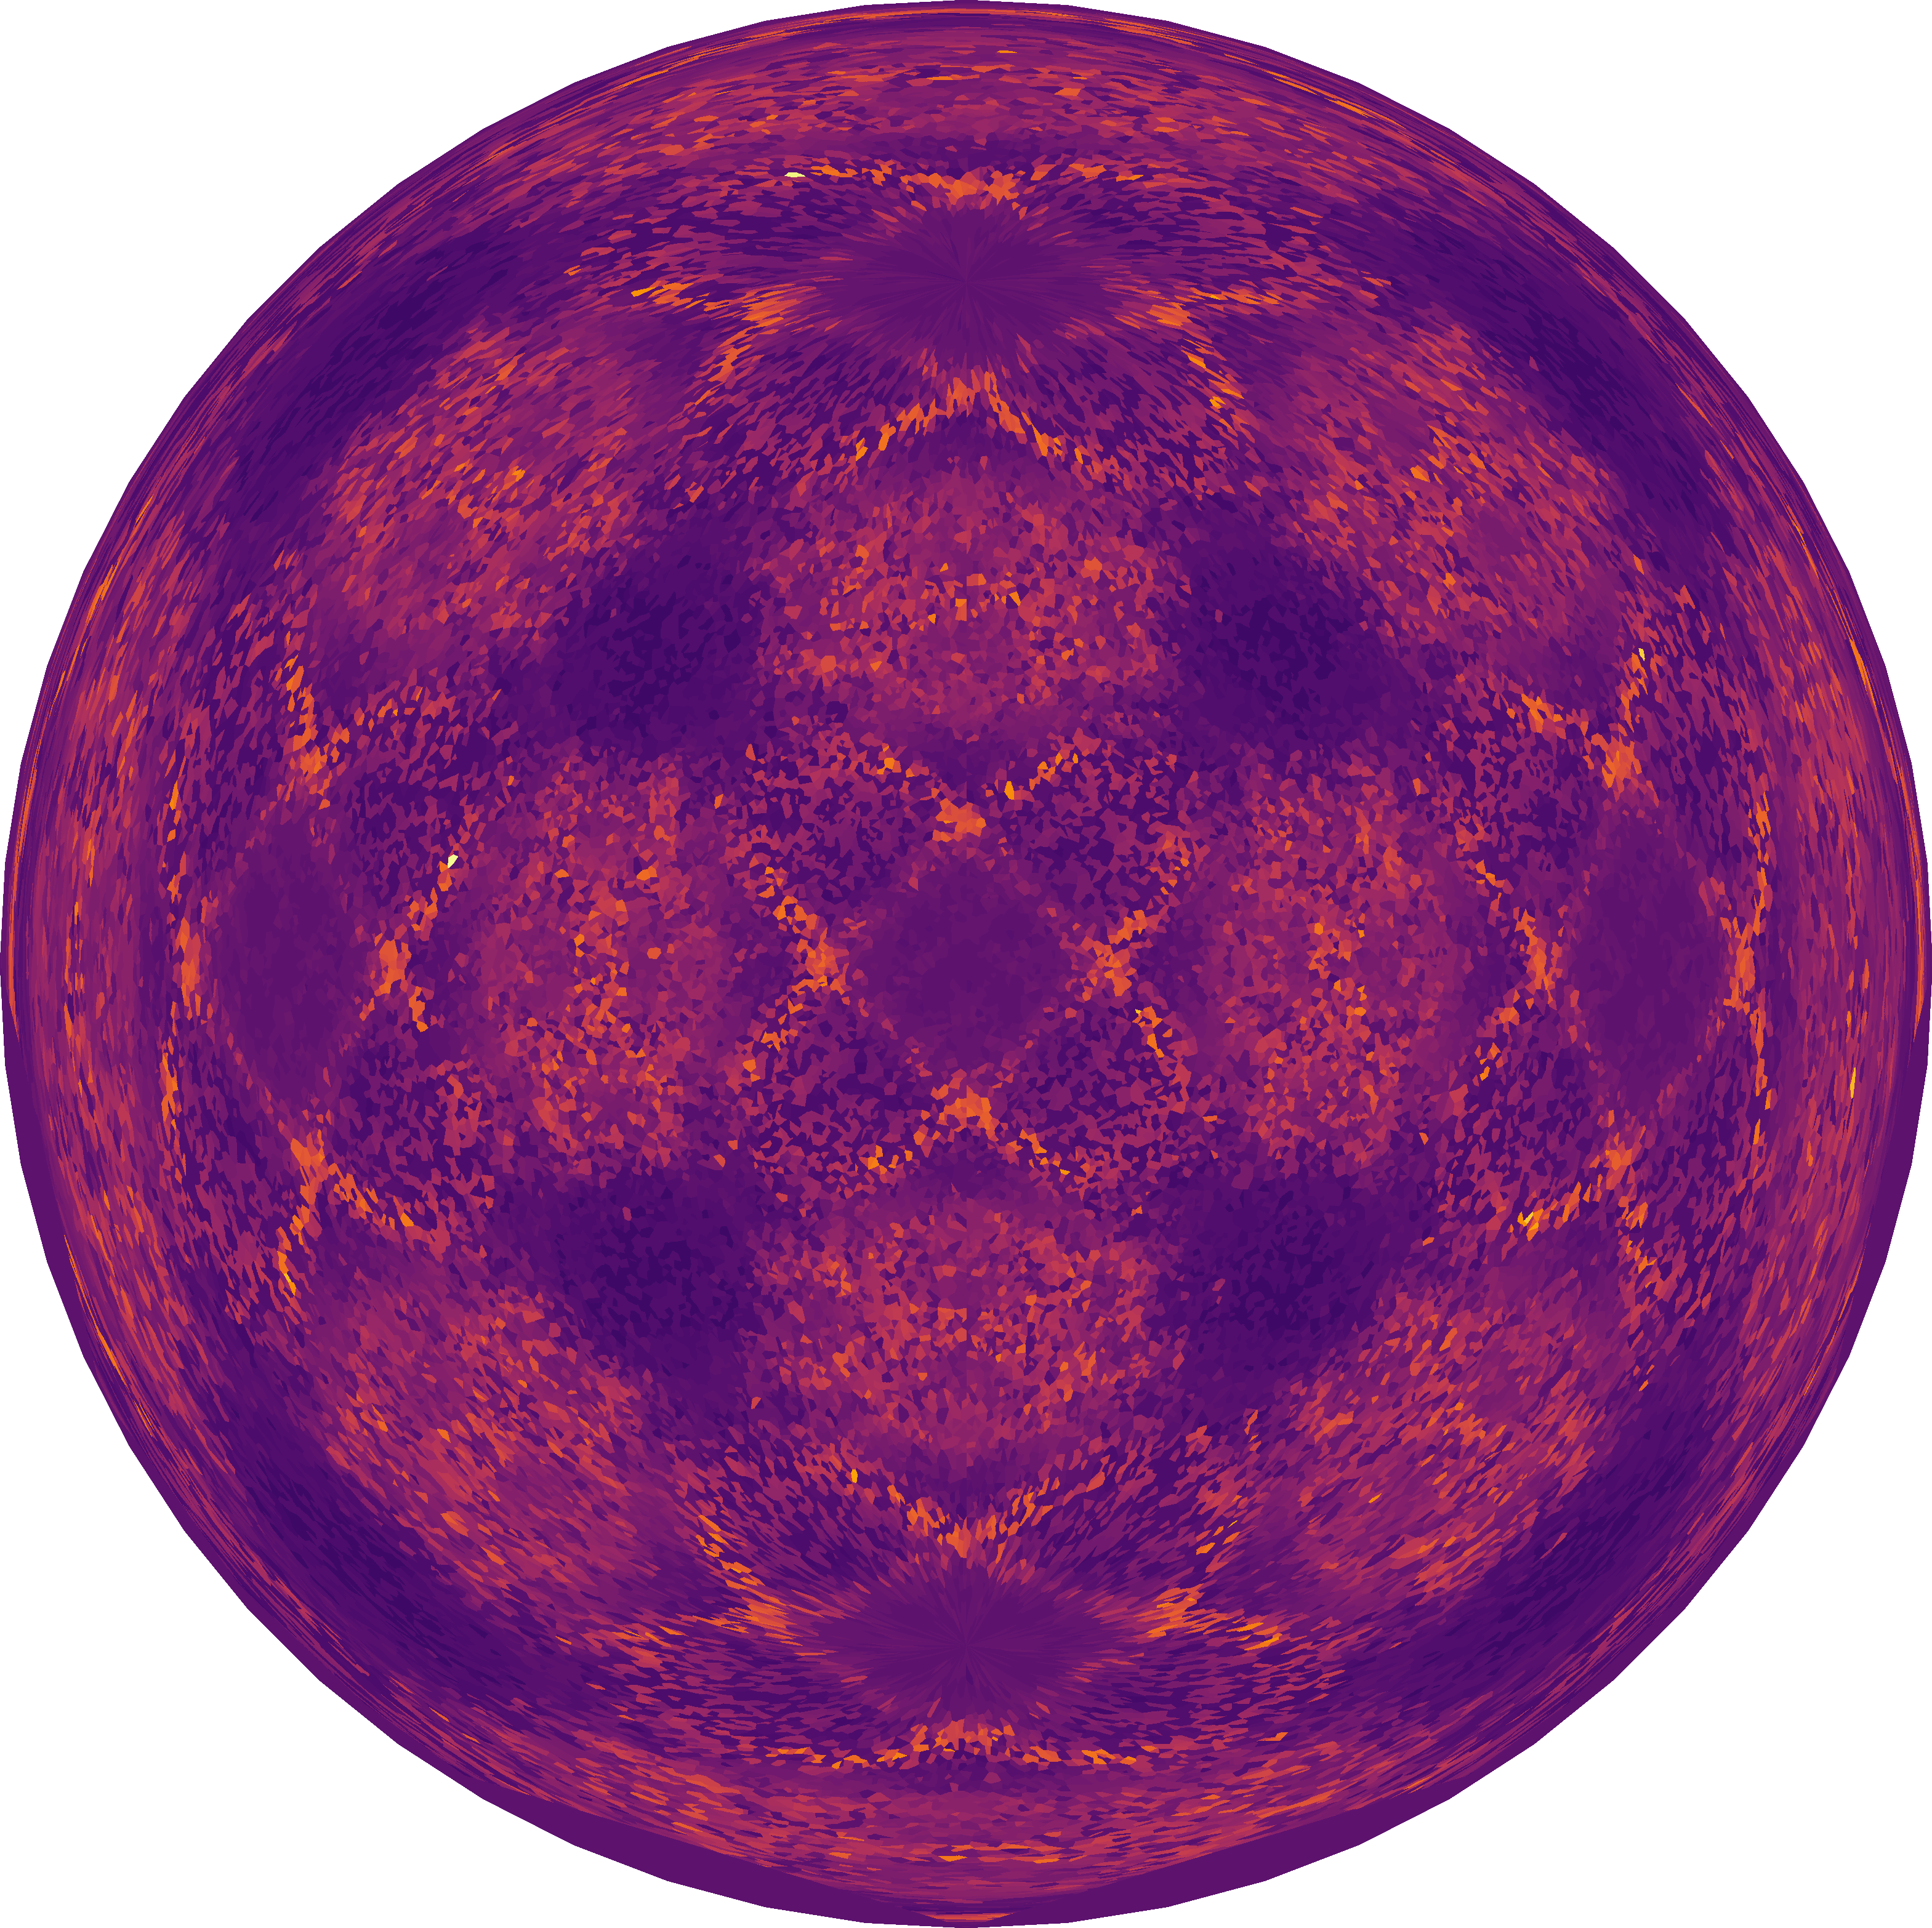
\includegraphics[width=0.95\textwidth]{surfaces/Ge_lambert_aea.png}
            };
            \addplot+ [mark = none, solid, color = \infernoaxiscolor]
                table {surfaces/horizontal_line_0.dat};
            \addplot+ [mark = none, solid, color = \infernoaxiscolor]
                table {surfaces/horizontal_line_1.dat};
            \addplot+ [mark = none, solid, color = \infernoaxiscolor]
                table {surfaces/horizontal_line_2.dat};
            \addplot+ [mark = none, solid, color = \infernoaxiscolor]
                table {surfaces/horizontal_line_3.dat};
            \addplot+ [mark = none, solid, color = \infernoaxiscolor]
                table {surfaces/horizontal_line_4.dat};
            \addplot+ [mark = none, solid, color = \infernoaxiscolor]
                table {surfaces/vertical_line_0.dat};
            \addplot+ [mark = none, solid, color = \infernoaxiscolor]
                table {surfaces/vertical_line_1.dat};
            \addplot+ [mark = none, solid, color = \infernoaxiscolor]
                table {surfaces/vertical_line_2.dat};
            \addplot+ [mark = none, solid, color = \infernoaxiscolor]
                table {surfaces/vertical_line_3.dat};
            \addplot+ [mark = none, solid, color = \infernoaxiscolor]
                table {surfaces/vertical_line_4.dat};
        \end{axis}
    \end{tikzpicture}
    \caption{High-resolution map of the threshold displacement energy surface for germanium based on around 86,000 randomly sampled directions from \textcite{KadribasicEtAl2018} displayed using a Lambert azimuthal equal-area projection.}
    \label{fig:ge-threshold-energy}
\end{figure}

\chapter{Dark matter velocity distribution in the laboratory frame}
\label{chap:dist}

The present understanding of the distribution of dark matter is (to a first approximation) that galaxies, such as the Milky Way, are situated inside a roughly spherically symmetric halo of dark matter moving at nonrelativistic velocities following largely a Maxwellian velocity distribution stationary in the galactic frame. At a more granular level, substructures of local over and underdensities, streams, and other deviations from a spherical halo and Maxweillian velocity distribution are expected to exist. This general picture of the distribution of dark matter is formed from observations from galactic rotation curves \parencites{SofueEtAl1999, LelliMcGaughSchombert2016}, observations of structure of the Milky Way \parencites{PortailEtAl2016, LabiniEtAl2023, BelokurovEtAl2018, KruijssenEtAl2018, HelmiEtAl2018}, and simulations of structure formation \parencites{VogelsbergerEtAl2014, WangEtAl2015, KlypinEtAl2016, SpringelEtAl2017, SpringelEtAl2008, DiemandEtAl2008, StadelEtAl2009, vandenBoschOgiya2018}.

Although it is generally understood that the distribution of dark matter in the galactic halo tends to be spherically symmetric, its precise radial profile is less well known. The observed flattening of the galactic rotation curves implies that at large radial distances, $r$, from the galactic center the density drops as $r^{-2}$. This conclusion follows from elementary Newtonian physics, as the circular velocity inside a spherically symmetric mass distribution at radial distance $r$ is given by
\begin{equation}
    v(r)=\sqrt{\frac{GM(r)}{r}},
\end{equation}
where $M(r)$ is the mass contained within the radius. The condition $v(r)=\text{const.}$ requires $M(r)\propto r$, which in the spherically symmetric case implies a density
\begin{equation}
    \rho(r)=\frac{1}{4\pi r^2}\der{M}{r}\propto r^{-2}.
\end{equation}
However, when it comes to the density at smaller radial distances, presently available observational data is compatible with a number of different density profiles. Plausible models for the density profile include those of \textcite{NavarroFrenkWhite1996}, Einasto \parencites{Einasto1965, MerrittEtAl2006}, \textcite{Burkert1995}, as well as the isothermal core profile \parencites{BahcallSoneira1980, BegemanBroeilsSanders1991}. Profiles can generally be divided into core profiles (isothermal core, Burkert), where the density profile flattens out at radii close to zero, and cuspy profiles which grow to a large value towards the galactic center (NFW, Einasto). It is worth noting that at present there exists tension between observations of galaxy rotation curves and galaxy formation over the shapes of the density profiles with observations preferring core profiles, while simulations prefer cuspy profiles. For discussion on this and other small scale structure issues, see a recent review by \textcite{TulinYu2018}.

Crucial from the point of view of direct detection experiments is the dark matter velocity distribution, $f(\vec{v})$, as it, in part, determines the directional and energy distribution of scattering events in a direct detection experiment. Commonly, the velocity distribution of dark matter is taken to be the end state of a violent relaxation, which mixes the energies of the particles in a stochastic process \parencite{LyndenBell1967}. The distribution of velocities is then one which maximizes the entropy under energy conservation; that is, the Maxwell--Boltzmann distribution, $f(\vec{v})\propto \exp(-v^2/2\sigma^2)$. However, in the long term, particles whose velocities exceed the escape velocity of the halo will get ejected from the system. Taking into account this process leads to the standard halo model (SHM) velocity distribution,
\begin{equation}
    f_\text{SHM}(\vec{v})\propto e^{-v^2/2\sigma^2}\Theta(v_\text{esc}-v).
    \label{eq:shm-dist}
\end{equation}

The standard halo model has traditionally been the velocity distribution assumed by the majority of direct detection studies because it is one of the few distributions for which~\eqref{eq:dm-master-rate} has nice closed form solutions. However, it is reasonable to expect the true velocity distribution to deviate from it in substantial ways. This is already somewhat evident from the abrupt cutoff at $v=v_\text{esc}$. An ad hoc model which removes the cutoff may be written as
\begin{equation}
    f(\vec{v})\propto(e^{-(v_\text{esc}^2-v^2)/2\sigma^2}-1)\Theta(v_\text{esc}-v).
\end{equation}
A generalization of this was given by \textcite{LisantiEtAl2011},
\begin{equation}
    f(\vec{v})\propto(e^{-(v_\text{esc}^2-v^2)/2k\sigma^2}-1)^k\Theta(v_\text{esc}-v),
\end{equation}
where a parameter value $k\in[1.5,3.5]$ was shown to fit the high velocity tail obtained from $N$-body simulations.

The velocity distributions discussed above all share the property of being isotropic. While isotropic distributions are computationally easier to handle, they are not motivated by $N$-body simulations or available data from the stellar neighborhood. Studies fitting separate radial and tangential parts,
\begin{equation}
    f(v_r)\propto e^{-(v_r^2/2\sigma_r^2)^{\alpha_r}},\quad f(v_t)\propto v_te^{-(v_t^2/2\sigma_t^2)^{\alpha_t}},
\end{equation}
onto data from various $N$-body simulations have found that the velocity dispersion in the radial direction tends to be greater than in the tangential direction \parencites{FairbairnSchwetz2009, KuhlenEtAl2010}. Furthermore, recent analysis of data gathered by the Gaia satellite suggests the presence of a ``sausage'' structure, which has been suggested to be the result of a past galaxy merger event \parencites{BelokurovEtAl2018, KruijssenEtAl2018, HelmiEtAl2018}. This sausage exhibits significant anisotropy  in the velocity space, with its isosurfaces forming elongated shapes which give it its name. Based on this model, \textcite{EvansOHareMcCabe2019} suggest the $\text{SHM}^{++}$ velocity distribution,
\begin{equation}
    f(\vec{v})=(1-\eta)f_R(\vec{v})+\eta f_S(\vec{v}),
\end{equation}
which consists of a round component $f_R(\vec{v})$ given by the SHM distribution~\eqref{eq:shm-dist} combined with a highly anisotropic sausage component,
\begin{equation}
    f_S(\vec{v})\propto\exp\left(-\frac{v_r^2}{2\sigma_r^2}-\frac{v_\theta^2}{2\sigma_\theta^2}-\frac{v_\varphi^2}{2\sigma_\varphi^2}\right).
\end{equation}
Here $\sigma_r$ is the radial velocity dispersion as before, while $\sigma_\theta$ and $\sigma_\varphi$ are the tangential and azimuthal dispersions, respectively, relative to the galactic plane. As before, the tangential and azimuthal dispersions are taken to be degenerate such that $\sigma_\theta=\sigma_\varphi$.

Beyond the overall shape of the dark matter halo and its typical velocity distribution, the true local galactic environment is a complex dynamic environment. The Milky Way is surrounded by a number of smaller satellite galaxies, and their existence suggests the presence of subhalos of dark matter within the larger galactic halo. These subhalos can get torn apart by tidal forces, which lead to dark matter streams: structures of dark matter with overall velocity relative to the galactic center, and small velocity dispersion. Some observational evidence for dark matter streams comes from observations of the Sagittarius stream \parencite{BelokurovEtAl2013} and from recent Gaia data \parencite{NecibLisantiBelokurov2019}. However, numerical simulations suggest the existence of many more streams \parencite{HelmiWhiteSpringel2002}. Although streams constitute a small part of the total mass of the dark matter halo, they can form a significant contribution to the local density if one happens to be passing through the Earth.

\section{Earth's motion and the dark matter halo}

The dark matter halo, by definition, should have no overall linear motion in the galactic frame, because the galactic coordinate system is defined as stationary relative to the galactic center of mass. The primary motion of dark matter in any neighborhood then comes from overall rotational motion of the halo, because the halo necessarily has some angular momentum. However, in the view where the galactic disk and dark matter halo formed from the same collapsing mass of baryons and dark matter, the rotational velocity of the halo should be negligible compared to that of the much more compact galactic disk. More formally, one can define the dimensionless spin parameter $\lambda=JE^{1/2}/GM^{5/2}$, where $J$, $E$, and $M$ are the total angular momentum, energy, and mass of the system, respectively, and $G$ is the gravitational constant. The spin parameter characterizes the portion of the system's energy stored in angular motion. Numerical simulations of galaxy formation find $\lambda_\text{disk}\gg\lambda_\text{halo}$, which supports the view that the rotational motion of the halo is small \parencites{MoMaoWhite1998, WarrenEtAl1992, KimmEtAl2011}. For this reason standard treatments of dark matter direct detection tend to neglect the rotational motion.

Attempts to observe scattering events of dark matter particles from the galactic halo are in the foreseeable future likely to take place in terrestrial laboratories. From the observer's perspective, then, regardless of what minor angular motion the halo has, the dark matter appears to be coming at us at the same speed with which Earth moves through the galaxy. The immediate consequence of this is that the mean of the velocity distribution in the laboratory coordinates is shifted such that $f(\vec{v})\rightarrow f(\vec{v}+\vec{v}_\text{lab})$, where $\vec{v}_\text{lab}$ is the velocity of the laboratory frame relative to the galactic frame. In addition, relevant for direct detection experiments with any kind of sensitivity to the direction of the incoming dark matter particles is the orientation of the laboratory frame with respect to the galactic frame, which for any terrestrial frame is not constant due to the rotation of the Earth. Full understanding of these coordinate transformations is therefore imperative for prediction and interpretation of potential direct detection signals.

The decomposition of $\vec{v}_\text{lab}$ to well-understood components is straightforward. The greatest contribution comes from the rotational motion of the Milky Way galaxy, which gives for the mean motion of the local neighborhood of the solar system the circular velocity, $\vec{v}_\text{circ}$, with an observed magnitude of around 220--240 km/s. The solar system has some peculiar motion relative to its surroundings, which introduces a correction $\vec{v}_\text{pec}$ to the velocity. The combination of these two velocities gives the center of mass velocity of the solar system. An observer on Earth then has two motions with respect to the rest frame of the solar system: the orbital velocity of the Earth, $\vec{v}_\text{orb}$, and rotational velocity of a point on the Earth's surface, $\vec{v}_\text{rot}$, from the rotation of the Earth about its axis. Of these the orbital velocity, $\vec{v}_\text{orb}$, has a magnitude around 30 km/s, and therefore has a significant contribution to $\vec{v}_\text{lab}$ which produces the well-known and sought for annual modulation of the dark matter direct detection signal. The magnitude of $\vec{v}_\text{rot}$ is at most about 0.46 km/s. In principle its presence induces a daily modulation of the direct detection signal via the same principle as the annual modulation signal. However, because of its small amplitude, this signal is unlikely to be detectable by any experiment in the foreseeable future. In any case, in summary, $\vec{v}_\text{lab}$ has the decomposition
\begin{equation}
    \vec{v}_\text{lab}=\vec{v}_\text{circ}+\vec{v}_\text{pec}+\vec{v}_\text{orb}+\vec{v}_\text{rot}.
\end{equation}
It is useful to combine the two approximately constant components, $\vec{v}_\text{circ}$ and $\vec{v}_\text{pec}$, into a single component $\vec{v}_\text{sol}=\vec{v}_\text{circ}+\vec{v}_\text{pec}$, the velocity of the solar system in the galactic frame, such that
\begin{equation}
    \vec{v}_\text{lab}=\vec{v}_\text{sol}+\vec{v}_\text{orb}+\vec{v}_\text{rot}.
\end{equation}

\begin{table}
    \begin{tblr}[
        tall,
        caption = {Coordinate systems for transforming between the galactic frame and a lab frame.},
        label = {tab:coordsys},
        note{*} = {The axes as defined in the ICRS deviate from the J2000.0 north celestial pole and March equinox by $\sim0.01''$. This deviation is insignificant for this work and is neglected for sake of simplicity.},
        remark{Note} = {All coordinate systems are right-handed by convention and therefore completely defined by their $z$- and $x$-axes. The orientation of the DCS is not defined because it depends on the specifics of the detector type. The GCS is defined as being centered on the Sun at any given moment, but is defined to be stationary in the sense that it has no velocity relative to the galactic center. J2000.0 is the reference epoch for the ICRS axes.}]
    {
        colspec = {X[l]X[l]X[l]X[l]},
        hline{1,Z} = {0.08em},
        hline{2} = {0.05em}
    }
        Coordinate system & Center & $z$-direction & $x$-direction\\
        Galactic coordinate system (GCS) & Solar system barycenter & North galactic pole & Galactic center \\
        International Celestial Reference System (ICRS) & Solar system barycenter & North celestial pole (J2000.0)\TblrNote{*} & March equinox (J2000.0)\TblrNote{*} \\
        Horizontal coordinate system (HCS) & Detector & Zenith & North \\
        Detector coordinate system (DCS) & Detector & --- & ---\\
    \end{tblr}
\end{table}

The relevant coordinate system definitions for transforming between the laboratory frame and the galactic frame are summarized in table \ref{tab:coordsys}. The sequence of transformations from the galactic frame to the frame of the detector proceeds from top to bottom. First, the dark matter velocity distribution is transformed from the galactic coordinate system (GCS) to the International Celestial Reference System (ICRS), which is the standard celestial coordinate reference system. The ICRS closely resembles the traditional equatorial coordinate system, but is defined to be nonrotating with respect to distant extragalactic radio sources, as defined by the International Earth Rotation and Reference Systems Service (IERS) \parencite{MaFeissel1997}. From the ICRS, to get to a frame corresponding to an Earth-based laboratory, a transformation is made to the horizontal coordinate system (HCS). From here a transformation is made to the detector coordinate system (DCS), which is the laboratory frame in which the dark matter scattering is described. The exact definition of the DCS is arbitrary, and depends on what is a useful coordinate system for describing a given direct detection experiment. In the case of a crystalline detector with a detection anisotropy that exhibits the symmetries of the crystal, for example, this might be a coordinate system whose axes are perpendicular to the walls of the crystals rectangular unit cell. The transformation between the HCS and DCS is then a rotation that depends on the exact orientation of the detector crystal. This would be relevant in the context of a specific detector, but in a generic theoretical analysis of detector concepts, we lose no valuable insight by assuming $\text{HCS}=\text{DCS}$ for simplicity.

For the purposes of this analysis, all transformations are described as Galilean transformations consisting of a rotation---given by a matrix, $R$---and a boost---given by a velocity, $\vec{v}$. (The translational part of the coordinate transformations is not relevant for analysis of dark matter scattering.)

Due to the complexities arising from many-body interactions in the solar system, as well as from motions of the Earth's crust, precise definitions of the transformation between the ICRS and HCS involve various corrections of different orders of magnitude. Given that the present state of dark matter direct detection is that no experiment has observed a confirmed dark matter signal to begin with, that any potential observed signal would be weak and subject to large uncertainties, that existing directional detection technologies have poor angular resolution, and that there are significant uncertainties in the parameters of the GCS to ICRS transformation already, a highly accurate determination of the ICRS to HCS transformation is hardly necessary. Therefore, for the purposes of this work, we can safely ignore angular corrections that result in corrections significantly less than 1\degree{} per century or $40''$ per year.

\section{Coordinates: GCS to ICRS}

The galactic coordinate system (GCS) is defined as a coordinate system centered on the Sun, which has its $z$-axis perpendicular to the galactic plane, towards the galactic north pole, and its $x$-axis towards the galactic center. Although it is defined to be centered on the Sun at any given moment, it is defined to have no velocity relative to the galactic center, and therefore it functions as a rest frame for the dark matter halo. Its orientation relative to the ICRS is completely described by three observable angles: the right ascension, $\alpha_\text{NGP}$, and declination, $\delta_\text{NGP}$, of the north galactic pole (NGP), as well as the galactic longitude, $\ell_\text{NCP}$, of the north celestial pole (NCP). The latter is expressed in galactic coordinates, but from figure~\ref{fig:galtrans} can be easily seen to equal the position angle of the galactic center. Recent observational values of these angles provided by \cite{KarimMamajek2017} are shown in table~\ref{tab:gcs}.

\begin{figure}
    \center
    \tdplotsetmaincoords{60}{-45}
    \newcommand{\galcolor}{\secondarylinecolor}
    \newcommand{\equcolor}{\primarylinecolor}
    \newcommand{\intercolor}{black}
    \newcommand{\fadecolor}{black!20!white}
    \begin{tikzpicture}[tdplot_main_coords, scale = 1.1]
        \draw [thick, ->, \equcolor]
            (0,0,0)--(3,0,0)node[anchor=south west]{$x$};
        \draw [thick, ->, \equcolor]
            (0,0,0)--(0,3,0)node[anchor=south east]{$y$};
        \draw [thick, ->, \equcolor]
            (0,0,0)--(0,0,3)node[anchor=south]{NCP};
        \draw [thick, dashed]
            (0,0,0)--(-2.605,-0.5892,0)--(-2.605,-0.5892,1.466);
        \tdplotdrawarc [\fadecolor] {(0,0,0)}{3}{0}{360}{}{};
        \tdplotdrawarc [thick, dashed] {(0,0,0)}{0.5}{0}{192.7}{anchor = south}{$\alpha_\text{NGP}$};
        \tdplotsetrotatedcoords{90}{90}{90};
        \tdplotdrawarc [thick, tdplot_rotated_coords, dashed]{(0,0,0)}{0.8}{0}{27.087}{anchor = north east}{$\delta_\text{NGP}$};
        %\tdplotsetrotatedcoords{0}{0}{192.7};
        %\draw[tdplot_rotated_coords,->](0,0,0)--(3,0,0)node[anchor=north]{$x''$};
        %\draw[tdplot_rotated_coords,->](0,0,0)--(0,3,0)node[anchor=east]{$y''$};
        %\draw[tdplot_rotated_coords,->](0,0,0)--(0,0,3)node[anchor=east]{$z''$};
        \tdplotsetrotatedcoords{12.7}{-62.916}{0};
        %\draw[thick,\intercolor,tdplot_rotated_coords,->](0,0,0)--(3,0,0)node[anchor=south]{$x'$};
        %\draw[thick,\intercolor,tdplot_rotated_coords,->](0,0,0)--(0,3,0)node[anchor=south east]{$y'$};
        \draw [thick,\galcolor,tdplot_rotated_coords,->]
            (0,0,0)--(0,0,3) node [anchor = east] {NGP};
        %\draw[thick,tdplot_rotated_coords,->](0,0,0)--(0,-3,0)node[anchor=north west]{\ascnode};
        \tdplotdrawarc [\fadecolor,thick,tdplot_rotated_coords]{(0,0,0)}{3}{0}{360}{}{};
        \tdplotsetrotatedcoords{12.7}{-62.916}{237.07};
        \draw [thick,\galcolor,tdplot_rotated_coords,->]
            (0,0,0)--(3,0,0) node [anchor = north] {GC};
        \draw [thick,\galcolor,tdplot_rotated_coords,->]
            (0,0,0)--(0,3,0) node [anchor = south west] {$y'$};
        %\tdplotdrawarc[thick,tdplot_rotated_coords,dashed]{(0,0,0)}{0.8}{0}{32.93}{anchor=north west}{$\ell_0$};
        \tdplotdrawarc [thick, tdplot_rotated_coords, dashed]{(0,0,0)}{0.6}{0}{122.93}{anchor=north west}{$\ell_\text{NCP}$};
        \tdplotsetrotatedcoords{102.7}{-90}{0};
        \tdplotdrawarc[\fadecolor, thick, tdplot_rotated_coords]{(0,0,0)}{3}{0}{360}{}{};
        \tdplotsetrotatedcoords{137.848}{-41.67}{0};
        \tdplotdrawarc[\fadecolor, thick, tdplot_rotated_coords]{(0,0,0)}{3}{0}{360}{}{};
        \tdplotsetrotatedcoords{12.7}{-62.916}{180};
        \coordinate (Shift) at (-2.605,-0.5892,1.466);
        \tdplotsetrotatedcoordsorigin{(Shift)}
        %\tdplotdrawarc[thick,tdplot_rotated_coords,dashed]{(0,0,0)}{0.4}{0}{-122.93}{anchor=north east}{PA};
    \end{tikzpicture}
    \caption{Comparison of the equatorial and galactic coordinate systems. Orange axes are the GCS axes, and the blue axes are the ICRS axes. The angles $\alpha_\text{NGP}$ and $\delta_\text{NGP}$ are the right ascension and declination of the north galactic pole, respectively. Special labeled directions are the north galactic pole (NGP), galactic center (GC), and north celestial pole (NCP). The angle $\ell_\text{NCP}$ is the galactic longitude of the north celestial pole.}
    \label{fig:galtrans}
\end{figure}

\begin{table}\center
    \begin{tblr}[
        tall,
        label = {tab:gcs},
        caption = {Values of quantities defining the galactic coordinate system.},
        remark{Sources} = {The values for the top three parameters are from \textcite{KarimMamajek2017}. The value of the peculiar velocity is the commonly used value from \textcite{SchonrichBinneyDehnen2010}. A compilation of alternative values are given by \textcite{Coskunoglu2011}. The local circular velocity is not precisely known, so a range containing commonly used values is given; see text for details.}]
    {
        hspan = default,
        colspec = {lXl},
        width = \linewidth,
        hline{1,Z} = {0.08em},
        hline{2} = {0.05em}
    }
        Parameter & Units & Value \\
        $\alpha_\text{NGP}$ & degrees & $192.729\pm0.035$\\
        $\delta_\text{NGP}$ & degrees & $27.084\pm0.023$\\
        $\ell_\text{NCP}$ & degrees & $122.928\pm0.016$\\
        $\vec{v}_\text{pec}$ & km/s & $(11.1^{+0.69}_{-0.75},12.24^{+0.47}_{-0.47},7.25^{+0.37}_{-0.36})$\\
        $v_\text{circ}$ & km/s & 220--240\\
    \end{tblr}
\end{table}

The three angles given completely specify the rotational part of the transformation: a clockwise rotation about the $z$-axis by $\ell_\text{NCP}$, followed by a clockwise rotation about the $y$-axis by $\pi/2-\delta_\text{NGP}$, and finally a counterclockwise rotation about the $z$-axis by $\alpha_\text{NGP}-\pi$. These correspond to the rotations
\begin{equation}
    R_{\text{GCS}\rightarrow\text{ICRS}}=R_Z(\alpha_\text{NGP}-\pi)R_Y(\delta_\text{NGP}-\pi/2)R_Z(-\ell_\text{NCP}).
\end{equation}

The boost part of the GCS to ICRS transform is just $\vec{v}_\text{circ}+\vec{v}_\text{pec}$. Here we define $\vec{v}_\text{circ}$ in terms of its GCS coordinates as the vector $(0,v_\text{circ},0)$. Table~\ref{tab:gcs} also lists the observationally determined values for $\vec{v}_\text{pec}$ and $v_\text{circ}$ in the GCS. The peculiar velocity, $\vec{v}_\text{pec}$, is challenging to determine and there are multiple estimates of its value. The value listed in the table is that of \textcite{SchonrichBinneyDehnen2010}, but \textcite{Coskunoglu2011} lists values obtained by other studies. Some disagreement exists in the literature over the value of $v_\text{circ}$, owing to uncertainties in modeling the rotation curve of the Milky Way \parencite{McMillanBinney2009}. Most dark matter literature historically uses the value 220 km/s, which is close to the value $218\pm6$ km/s reported by \textcite{Bovy2012}. However, recent analyzes favor a value $233\pm3$ km/s \parencites{McMillan2017, EvansOHareMcCabe2019}.

\section{Coordinates: ICRS to DCS}

The transformation between the ICRS and HCS is conceptually and computationally more complicated than the transformation between GCS and ICRS, because it first involves a transformation into a frame that both travels and rotates with the Earth, and then a transformation to a frame that corresponds to an observer on the surface of the Earth, involving the relevant rotation and boost. The first part of the transformation consists of a boost by the Earth's orbital velocity $\vec{v}_\text{orb}$. Computing it is an exercise in basic Keplerian orbits. The displacement vector of an orbiting body from the locus of the orbit in the orbital plane is
\begin{equation}
    \vec{r}(t)=(r(\nu(t))\cos\nu(t),r(\nu(t))\sin\nu(t)).
    \label{eq:keplerdisp}
\end{equation}
The radial distance here is given by
\begin{equation}
    r(\nu)=\frac{a(1-e^2)}{1+e\cos\nu},
\end{equation}
where $a$ is the semi-major axis of the orbit, $e$ is the orbital eccentricity, and $\nu(t)$ is the true anomaly at time $t$. We can express equation~\eqref{eq:keplerdisp} in terms of the eccentric anomaly $E(t)$ of the orbit via
\begin{equation}
    \cos\nu=\frac{\cos E(t)-e}{1-e\cos E(t)},\qquad\sin\nu=\frac{\sqrt{1-e^2}\sin E(t)}{1-e\cos E(t)},
\end{equation}
whose time dependence in turn can be computed from the mean anomaly, $M(t)=M_0+2\pi(t-t_0)$, via Kepler's equation
\begin{equation}
    E(t)-e\sin E(t)=M(t).
\end{equation}
Here $t_0$ is the epoch at which $M=M_0$. The orbital velocity is then straightforward to compute by differentiating equation~\eqref{eq:keplerdisp} and using conservation of orbital angular momentum to obtain
\begin{equation}
    \vec{v}_\text{orb}(t)=\left(-\frac{2\pi}{T}\frac{a}{\sqrt{1-e^2}}\sin\nu(t),\frac{2\pi}{T}\frac{a}{\sqrt{1-e^2}}(e+\cos\nu(t))\right),
    \label{eq:vorbkep}
\end{equation}
where $T$ is the orbital period.

The coordinates of equation~\eqref{eq:vorbkep} are given in the orbital plane, centered on the Sun, with the $x$-axis aligned in the direction of the perihelion. For purposes of performing the boost with this velocity, we need to translate it to the ICRS. The necessary rotation can be written in terms of the argument of perihelion, $\omega$, the obliquity of the orbital plane, $\bar{\phi}$, and longitude of ascending node, $\Omega$, of the orbit at time $t$. These quantities evolve with time due to the precession of the orbital plane, but the rates of their evolution are below $50''$ per century. It is, therefore, sufficient to assume their J2000.0 values. The value of $\Omega$ in this case is approximately zero, so the relevant rotation is
\begin{equation}
    R_{\text{kep}\rightarrow\text{ICRS}}\approx R_X(\varepsilon_\text{J2000.0})R_Z(\omega_\text{J2000.0}).
\end{equation}

The boost by Earth's orbital velocity effectively takes us to the Geocentric Celestial Reference System (GCRS), which is effectively a geocentric alternative to the ICRS. The next step in the transformation procedure towards the HCS is an intermediate transformation to the International Terrestrial Reference System (ITRS), which is defined as a geocentric system having no rotation with respect to the Earth's surface. The transformation between the GCRS and ITRS is described in detail in the IERS Conventions \parencite{LuzumPetit2010}. It relies on two intermediate coordinate systems. First, the GCRS is transformed to the Celestial Intermediate Coordinate System (CIRS). The purpose of this transformation, and of the CIRS, is to account for the precession and nutation of the Earth's axis of rotation. The transformation then proceeds to the Terrestrial Intermediate Coordinate System (TIRS), which rotates with the Earth. The transformation between the TIRS and ITRS accounts for the motion of the Earth's rotational axis relative to its crust (polar motion).

The precession, nutation, and polar motion are exceedingly small effects. The polar motion has a period on the order of years with an amplitude around $0.5''$, while the nutation components are on the order of arcseconds. The precession progresses slowly at a rate of tens of arcseconds per year, and therefore its effect can be expected to not exceed multiple arcminutes over this century. Considering the present state of dark matter direct detection experiments, this level of accuracy in the orientation of the coordinate system is not necessary in any foreseeable future. Therefore, for our purposes, it is sufficient to only account for the rotation of the Earth. For the desired level of accuracy, the rotation then reduces to
\begin{equation}
    R_{\text{GRCS}\rightarrow\text{ITRS}}\approx R_Z(-\text{ERA}),
\end{equation}
where $ERA$ is the Earth rotation angle \parencite{LuzumPetit2010},
\begin{equation}
    \text{ERA}=2\pi(0.7790572732640+1.00273781191135448\cdot\text{UT1}_\text{J2000.0}).
\end{equation}
Here $\text{UT1}_\text{J2000.0}$ refers to the Universal Time defined with the origin $\text{UT1}_\text{J2000.0}=0$ on the J2000.0 epoch, January 1st, 2000, at 12:00 Terrestrial Time. UT1 is related to the Coordinated Universal Time (UTC) by the condition $|\text{UT1}-\text{UTC}|<0.9$ s, which is ensured by the addition of leap seconds to UTC. For practical purposes, in direct detection experiments we can therefore assume $\text{UT1}\approx\text{UTC}$.

From the ITRS, the coordinates are next rotated to the orientation of the HCS at some latitude, $\lambda$, and longitude, $\varphi$. To be precise, by definition of the $z$-axis of the HCS being defined by the zenith direction, the appropriate notion of latitude to use in this case is the astronomical latitude, determined by the angle of local gravitational acceleration relative to the equatorial plane. However, the deviations of astronomical latitude from the geodetic latitude (angle of surface normal of the reference ellipsoid to the equatorial plane) are on the order of arcseconds, so geodetic latitude is sufficient for direct detection experiments. Once the appropriate definition of latitude has been chosen, the corresponding rotation is given by
\begin{equation}
    R_{\text{ITRS}\rightarrow\text{HCS}}=R_Y(\tfrac{\pi}{2}-\lambda)R_Z(-\varphi).
\end{equation}
After the rotation to the correct orientation, the coordinate system needs to be boosted eastward to account for the rotation of the Earth---i.e., with velocity $\vec{v}_\text{rot}=(0,-v_\text{rot},0)$. Since this is already a subdominant correction to the total velocity, $\vec{v}_\text{lab}$, we may assume a spherical model of the Earth, in which case $v_\text{rot}=R_0\cos\lambda$, where $R_0$ denotes the mean radius of the Earth.

Without further specification of the detector setup, the transformation between the HCS and DCS may bee any general rotation matrix. Given the unit vectors $\unitv{x}_\text{DCS}$, $\unitv{y}_\text{DCS}$ and $\unitv{z}_\text{DCS}$ defining the axes of the DCS, expressed in HCS coordinates, this rotation matrix is
\begin{equation}
    R_{\text{HCS}\rightarrow\text{DCS}}=
    (
        \unitv{x}_\text{DCS},
        \unitv{y}_\text{DCS},
        \unitv{z}_\text{DCS}
    )^\transp.
\end{equation}
Appropriate definition of the DCS depends on the problem at hand. In general, the orientation of the coordinate system is only relevant if the detector has some known anisotropy that makes the signal sensitive to the orientation of the detector. The DCS should be defined in a manner which is both possible for an experiment to determine and relate to the HCS, and sufficiently unambiguous in the context of the theoretical description of the detector anisotropy. For example, in the context of anisotropy derived from the lattice structure of a cubic crystal the DCS axes could be the axes of the unit cell.

\section{Observational consequences of Earth's motion}

The motion of an Earth-based detector relative to the dark matter distribution means that for an observer on Earth the dark matter halo appears as dark matter wind hitting the Earth at velocity $\vec{v}_\text{DM}=-\vec{v}_\text{lab}$. In a hypothetical directional direct detection experiment this would imply the angular distribution of recoil events having a peak in the direction of $\vec{v}_\text{DM}$. This can be seen by considering equation~\eqref{eq:dm-master-rate} in the simple case of nucleon scattering with a $\tmean{|\mathcal{M}|^2}\sim 1$ interaction with an isotropic velocity distribution. The relevant part of the equation is
\begin{equation}
    \ddder{R_S}{E}{\Omega}\sim\int\delta\left(\vec{v}\cdot\unitv{q}+v_\text{min}\right)f(\vec{v}+\vec{v}_\text{lab})\difd^3v.
\end{equation}
A change of variables $\vec{v}'=\vec{v}+\vec{v}_\text{lab}$ in the integral, and a solution of the trivial angular part, then gives
\begin{equation}
    \ddder{R_S}{E}{\Omega}\sim\int_{|\vec{v}_\text{lab}\cdot\unitv{q}+v_\text{min}|}^\infty\hspace{-3em}vf(v)\difd v.
    \label{eq:isotropic-rate}
\end{equation}
Since $vf(v)$ is positive, the integral is monotonic as a function of the lower limit. Therefore, as a function of $v_\text{min}\sim E^{1/2}$, it reaches a maximum at $v_\text{min}=\max\{0,-\vec{v}_\text{lab}\cdot\unitv{q}\}$. It follows that the energy integrated event rate, $dR_S/d\Omega$, reaches a maximum when $-\vec{v}_\text{lab}\cdot\unitv{q}=v_\text{lab}$; that is, when $\unitv{q}=-\unitv{v}_\text{lab}$.

Such an anisotropy, whose direction remains fixed relative to the distant stars, opposing the motion of the solar system through the galaxy, would be a smoking gun signal for direct detection of dark matter. However, detectors with directional capabilities do exist at a scale yet where they would have any chance of observing the dark matter wind. Therefore, evidence of nonterrestrial origin of direct detection signals must be sought by other means.

In the absence of any directional sensitivity, it is evident from the above considerations that the total scattering rate, $R_S$, is larger for larger magnitudes of $\vec{v}_\text{lab}$. Therefore, any modulation of the magnitude $v_\text{lab}$ gets translated into a modulation of $R_S$ whose maximum coincides with the maximum of $v_\text{lab}$. The primary modulation component comes from the term $\vec{v}_\text{sol}+\vec{v}_\text{orb}$, where $\vec{v}_\text{orb}$ rotates in the Earth's orbital plane. This leads to an annual modulation in the magnitude of $\vec{v}_\text{lab}$, and, consequently, in the scattering rate, with the maximum occurring in the summer. This annual modulation offers the most well-studied feature of the signal which could allow discrimination of a dark matter signal from other naturally occurring backgrounds, since other sources of annual modulation with the same phase are difficult, although not impossible, to come up with.

Observation of an annual modulation signal with the desired phase has famously been claimed by the DAMA/LIBRA experiment since the early 2000s, with a presently stated significance of $13.7\sigma$ \parencite{BernabeiEtAl2023}. However, other experiments built to test the results of DAMA/LIBRA, using the same NaI scintillator crystals, have not observed an annual modulation \parencites{DMIce2017, COSINE1002019, COSINE1002024, KIMS2019, ANAIS2024}. Furthermore, the best-fit region of the dark matter fit for the signal is ruled out by multiple other experiments as shown in figure~\ref{fig:dd-reach}.  These results are difficult to reconcile with a dark matter interpretation of the DAMA/LIBRA signal.

There is, in principle, also a daily modulation signal arising from the variation of the magnitude of $\vec{v}_\text{lab}$ when the rotational velocity, $\vec{v}_\text{rot}$, on the Earth's surface is taken into account. Given that the rotational velocity is, at its maximum around 0.46 km/s, this modulation is subdominant compared to the annual modulation. More common source of signal modulation, however, are anisotropies in the detector response. If we multiply equation~\eqref{eq:isotropic-rate} by a direction dependent response factor, $S(E,\unitv{q})$, whose orientation is fixed relative to the laboratory frame, then the effect of the response factor on the event rate varies as the Earth rotates about its axis, leading to a daily variation in the event rate.

\begin{figure}
    \center
    \begin{tikzpicture}
        \pgfplotsset{point meta min=1, point meta max=13.0}
        \begin{axis}[
                scale only axis = true,
                height = 0.99\textwidth,
                axis y line = none,
                axis x line = none,
                axis line style = {draw = white},
                title style = {at = {(0.5,0.9)}},
                width = 0.99\textwidth,
                ymin = -2.0,
                ymax = 2.0,
                xmin = -2.0,
                xmax = 2.0,
                every axis plot/.append style = {line width = 1.0pt},
                colormap name = twilight,
                colorbar,
                colorbar horizontal,
                colorbar style = {
                    at = {(0.5,-0.07)},
                    xlabel = Date,
                    xtick = {1, 2, 3, 4, 5, 6, 7, 8, 9, 10, 11, 12, 13},
                    xticklabels = {Jan, Feb, Mar, Apr, May, Jun, Jul, Aug, Sep, Oct, Nov, Dec, Jan},
                    width = 0.95*\pgfkeysvalueof{/pgfplots/parent axis width},
                    anchor = north},
                cycle list = {[samples of colormap = {13}]},
                name = border]
            \fill [color=\plotbgcolor]
                (axis cs:0,0) circle [radius = 2.0];
            \addlegendimage{no markers,grey};
            \label{legend.A};
            \addlegendimage{no markers,grey,dashed};
            \label{legend.B};
            \addplot+ [mark = none, solid, color = \plotfgcolor]
                table {surfaces/horizontal_line_0.dat};
            \addplot+ [mark = none, solid, color = \plotfgcolor]
                table {surfaces/horizontal_line_1.dat};
            \addplot+ [mark = none, solid, color = \plotfgcolor]
                table {surfaces/horizontal_line_2.dat};
            \addplot+ [mark = none, solid, color = \plotfgcolor]
                table {surfaces/horizontal_line_3.dat};
            \addplot+ [mark = none, solid, color = \plotfgcolor]
                table {surfaces/horizontal_line_4.dat};
            \addplot+ [mark = none, solid, color = \plotfgcolor]
                table {surfaces/vertical_line_0.dat};
            \addplot+ [mark = none, solid, color = \plotfgcolor]
                table {surfaces/vertical_line_1.dat};
            \addplot+ [mark = none, solid, color = \plotfgcolor]
                table {surfaces/vertical_line_2.dat};
            \addplot+ [mark = none, solid, color = \plotfgcolor]
                table {surfaces/vertical_line_3.dat};
            \addplot+ [mark = none, solid, color = \plotfgcolor]
                table {surfaces/vertical_line_4.dat};
            \pgfplotsset{cycle list shift = -10};
            \addplot+ [mark = none, solid]
                table {directions/dm_wind_dir_46.47186_-81.18669_2024-01-01_2024-01-01-23-50_lambert_aea.dat} -- cycle;
            \addplot+ [mark = none, solid]
                table {directions/dm_wind_dir_46.47186_-81.18669_2024-02-01_2024-02-01-23-50_lambert_aea.dat} -- cycle;
            \addplot+ [mark = none, solid]
                table {directions/dm_wind_dir_46.47186_-81.18669_2024-03-01_2024-03-01-23-50_lambert_aea.dat} -- cycle;
            \addplot+ [mark = none, solid]
                table {directions/dm_wind_dir_46.47186_-81.18669_2024-04-01_2024-04-01-23-50_lambert_aea.dat} -- cycle;
            \addplot+ [mark = none, solid]
                table {directions/dm_wind_dir_46.47186_-81.18669_2024-05-01_2024-05-01-23-50_lambert_aea.dat} -- cycle;
            \addplot+ [mark = none, solid]
                table {directions/dm_wind_dir_46.47186_-81.18669_2024-06-01_2024-06-01-23-50_lambert_aea.dat} -- cycle;
            \addplot+ [mark = none, solid]
                table {directions/dm_wind_dir_46.47186_-81.18669_2024-07-01_2024-07-01-23-50_lambert_aea.dat} -- cycle;
            \addplot+ [mark = none, solid]
                table {directions/dm_wind_dir_46.47186_-81.18669_2024-08-01_2024-08-01-23-50_lambert_aea.dat} -- cycle;
            \addplot+ [mark = none, solid]
                table {directions/dm_wind_dir_46.47186_-81.18669_2024-09-01_2024-09-01-23-50_lambert_aea.dat} -- cycle;
            \addplot+ [mark = none, solid]
                table {directions/dm_wind_dir_46.47186_-81.18669_2024-10-01_2024-10-01-23-50_lambert_aea.dat} -- cycle;
            \addplot+ [mark = none, solid]
                table {directions/dm_wind_dir_46.47186_-81.18669_2024-11-01_2024-11-01-23-50_lambert_aea.dat} -- cycle;
            \addplot+ [mark = none, solid]
                table {directions/dm_wind_dir_46.47186_-81.18669_2024-12-01_2024-12-01-23-50_lambert_aea.dat} -- cycle;
            \pgfplotsset{cycle list shift = -12};
            \addplot+ [mark = none, dashed]
                table {directions/sun_dir_46.47186_-81.18669_2024-01-01_2024-01-01-23-50_lambert_aea.dat} -- cycle;
            \addplot+ [mark = none, dashed]
                table {directions/sun_dir_46.47186_-81.18669_2024-02-01_2024-02-01-23-50_lambert_aea.dat} -- cycle;
            \addplot+ [mark = none, dashed]
                table {directions/sun_dir_46.47186_-81.18669_2024-03-01_2024-03-01-23-50_lambert_aea.dat} -- cycle;
            \addplot+ [mark = none, dashed]
                table {directions/sun_dir_46.47186_-81.18669_2024-04-01_2024-04-01-23-50_lambert_aea.dat} -- cycle;
            \addplot+ [mark = none, dashed]
                table {directions/sun_dir_46.47186_-81.18669_2024-05-01_2024-05-01-23-50_lambert_aea.dat} -- cycle;
            \addplot+ [mark = none, dashed]
                table {directions/sun_dir_46.47186_-81.18669_2024-06-01_2024-06-01-23-50_lambert_aea.dat} -- cycle;
            \addplot+ [mark = none, dashed]
                table {directions/sun_dir_46.47186_-81.18669_2024-07-01_2024-07-01-23-50_lambert_aea.dat} -- cycle;
            \addplot+ [mark = none, dashed]
                table {directions/sun_dir_46.47186_-81.18669_2024-08-01_2024-08-01-23-50_lambert_aea.dat} -- cycle;
            \addplot+ [mark = none, dashed]
                table {directions/sun_dir_46.47186_-81.18669_2024-09-01_2024-09-01-23-50_lambert_aea.dat} -- cycle;
            \addplot+ [mark = none, dashed]
                table {directions/sun_dir_46.47186_-81.18669_2024-10-01_2024-10-01-23-50_lambert_aea.dat} -- cycle;
            \addplot+ [mark = none, dashed]
                table {directions/sun_dir_46.47186_-81.18669_2024-11-01_2024-11-01-23-50_lambert_aea.dat} -- cycle;
            \addplot+ [mark = none, dashed]
                table {directions/sun_dir_46.47186_-81.18669_2024-12-01_2024-12-01-23-50_lambert_aea.dat} -- cycle;
            \node [
                    star,
                    star point ratio = 2.0,
                    scale = 0.5,
                    fill = \darkmarkcolor,
                    draw = \plotfgcolor,
                    thick] 
                at (0.000, 0.789) {};
            \node at (0.000, 0.789) [above right] {\small NCP};
        \end{axis}
        \newlength{\vlabdirwidth}
        \pgfextractx{\vlabdirwidth}{\pgfpointdiff{\pgfpointanchor{border}{west}}{\pgfpointanchor{border}{east}}}
        \addtolength{\vlabdirwidth}{-.696em}% inner sep
        \node[draw, below=3pt] at (border.south) {
            \begin{tblr}{
                hspan = minimal,
                rowsep = 0pt,
                colspec = {lX},
                width = 0.95\vlabdirwidth
            }
                \ref{legend.A} Incoming DM wind direction ($\unitv{v}_\text{lab}$) & \ref{legend.B} Solar direction ($\unitv{r}_\odot$) \\
            \end{tblr}
            %\makebox[0.95\vlabdirwidth]{\ref{legend.A} Incoming DM wind direction ($\unitv{v}_\text{lab}$)\hfil\ref{legend.B} Solar direction ($\unitv{r}_\odot$)}
        };
    \end{tikzpicture}
    \caption{Paths of the incoming dark matter wind direction (solid lines), and sun (dashed lines) on the first day of each month of the year 2024, as seen by a hypothetical observer at the location of the SNOLAB facility (46.47\degree N, 81.19\degree W) facing north, displayed using a Lambert azimuthal equal-area projection. The star marks the direction of the north celestial pole. The SNOLAB facility is the site of direct detection experiments from multiple collaborations, including \textcite{DEAP2016}, \textcite{PICO2016}, \textcite{SuperCDMS2017}, and \textcite{DAMIC2020}.}
    \label{fig:v-lab-dir}
\end{figure}

The daily modulation caused by detector response can be substantially more varied in nature than the annual modulation, or the daily modulation from variation of the magnitude $v_\text{lab}$. The latter two modulations generally have the same period as the motion that generates them: around 365 days (length of a sidereal year), and around 24 hours (length of a stellar day), respectively. However, the daily modulation due to the detector response, in general, consists of a combination of harmonics of the fundamental period of a stellar day. Depending on the shape of the detector response, and the orientation of the detector, any one of the harmonics may dominate, and therefore the dominant period of the modulation may also be half a stellar day, or third of a stellar day, or fourth of a stellar day, and so on.

A notable property of both types of daily modulation caused by the Earth's motion is that the phase of the signal varies throughout the year. Let $\vec{v}_E=\vec{v}_\text{sol}+\vec{v}_\text{orb}$ denote the center of mass velocity of Earth, and let $\vec{v}_E^\parallel$ be its component parallel to the equatorial plane. One period of daily modulation is then defined as the length of time it takes for the Earth to make one full revolution relative to $\vec{v}_E^\parallel$. If the direction of $\vec{v}_E^\parallel$ was constant, the daily modulation period would be exactly a stellar day. However, due to the time dependence of $\vec{v}_\text{orb}$, the direction of $\vec{v}_E^\parallel$ drifts throughout the year. This causes the period of daily modulation to vary slowly, which can be modeled as a time-dependent phase whose value is equal to the right ascension of the dark matter wind speed, $\alpha_w(t)$. Neglecting the small effect of Earth's axial tilt relative to the orbital plane, it is straightforward to show that the magnitude of the phase variation is approximately given by
\begin{equation}
    \Delta\alpha_w\approx 2\arcsin\left(\frac{|\vec{v}_\text{orb}^\parallel|}{|\vec{v}_\text{sol}^\parallel|}\right),
\end{equation}
which has a value of around 20\degree.

There is similarly a variation in the declination of the dark matter wind speed, $\delta_w(t)$, which results from variation in the velocity component $\vec{v}_E^\perp$ perpendicular to the orbital plane. This variation, of around 15\degree{}, can be seen in figure~\ref{fig:v-lab-dir} showing the daily paths of the direction of $\vec{v}_\text{lab}$ and solar direction, $\unitv{r}_\odot$, throughout the year as seen by an observer on Earth. This variation of the declination has the effect of slightly changing the profile of the daily modulation throughout the year.

Overall, the presence of these significant variations in both the declination and right ascension of the direction of $\vec{v}_\text{lab}$, in combination with the dependence of daily modulation on the orientation of the detector, makes the analysis of daily modulation substantially more complicated than the comparatively simple analysis of yearly modulation. Publication~\ref{pub:sassi2024} contains a detailed analysis on the variation in the daily modulation in germanium when the crystal orientation is changed. This analysis shows that the daily modulation can be dominated by completely different harmonics of the 24-hour period depending on the orientation of the crystal. That is, in one orientation the dominant period could be 12 hours, while in another it could be 6 hours. Furthermore, the dominant period depends on the degree of anisotropy in the velocity distribution. This complexity creates both challenges and opportunities. On one hand, the complex harmonic structure makes fitting daily modulation onto data far more difficult than in the case of annual modulation, and more assumptions are needed about the underlying model. On the other hand, the fact that daily modulation is sensitive to the model means that it could potentially be used to aid in model discrimination in the event of discovery of a signal.

The main goal of publication~\ref{pub:sassi2024} was to study whether daily modulation could be used aid in the discrimination of an SHM$^{++}$-style anisotropic component in the velocity distribution. More concretely, we assumed as a ``background'' model the SHM velocity distribution, and then used a likelihood analysis to investigate how small $\eta$, the fraction of the anisotropic component, could be to detect the presence of the anisotropy for a given number of recorded dark matter events. For the detector material and the source of daily modulation we used germanium and the ionization threshold anisotropy as in publication~\ref{pub:sassi2021}. We found that at $10^4$ recoil events, with an energy resolution of 10 eV, above a dark matter mass of 400 MeV, the anisotropic component was mainly revealed by its different recoil energy distribution due to its large tail of high velocity particles. In this case including temporal modulation effects did not improve the results. Below 400 MeV, however, annual modulation could improve the bounds on $\eta$ by at most around 10\%, and addition of daily modulation information would improve the bounds at most around 30\% over that. There was therefore a substantial gain from using daily modulation information, although in the mass range where the improvement was the greatest, the bounds never reached the SHM$^{++}$ compatible values of $\eta<0.3$.

We further tested a scenario, where we included some uncertainty over the dark matter interaction. That is, we included an uncertainty over whether the squared scattering amplitude was proportional to $|\vec{v}_\perp|^2$ or not. This was done because in preliminary investigations we had found that the effects of velocity dependence of the scattering amplitude on the daily modulation could resemble those of an anisotropic velocity component. However, this also brought uncertainty into the energy spectrum, and therefore the energy-only bounds for dark matter masses 400 MeV were significantly weakened. As expected, this also weakened the daily modulation bounds relative to the annual modulation bounds, with daily modulation information only giving at best a 15\% improvement this time.

The results of this study demonstrates the potential usefulness of daily modulation, but also indicates some of the same challenges observed in publication~\ref{pub:sassi2021} in relation to the use of the ionization threshold. Namely, because the daily modulation in this case is the result of not seeing scattering events below a certain energy threshold, the effect is highly energy dependent, and vanishes quickly when most of the scattering events have energies above the ionization threshold. We have demonstrated that daily modulation contains useful information about the direct detection signal, but sources of anisotropy that can produce daily modulation require further investigation.

\chapter{Discussion}

The past two decades have seen a great amount of development in the field of dark matter direct detection. The massive scaling up especially of the liquid noble detectors has allowed exploration of large parts of the parameter space. To make further progress they will likely have to contend with the background of neutrinos before they will discover evidence of dark matter. Development of new detector technologies, and refinement of existing ones, has meanwhile made it possible to search for scattering events at lower and lower energies. Recent progress on thermal phonon and ionization detector technologies using crystalline solid-state materials has made feasible the search for sub-GeV dark matter with recoil energies down to the electronvolt range \parencites{RomaniEtAl2018, CrislerEtAl2018, EDELWEISS2020}.

The development of these low-threshold detector technologies brings with it new challenges and opportunities. The electronvolt-scale energies probed by these detectors are of the order of atomic binding energies, and therefore the detector signal is highly sensitive to not just the properties of the target nuclei, but also to properties of the larger crystalline lattice structure formed by the nuclei. Understanding of these properties and their impact on the direct detection signal of dark matter has been a central part of this thesis.

Study of the effects of low-energy recoil events in crystals is a nontrivial task, and generally can only be done by means of direct simulation of the recoil events. A substantial part of this thesis is dedicated to the study of lattice defect formation from low-energy recoil events, because it relates to both the energy loss, and the ionization threshold energy in nuclear recoil events in crystalline solid-state materials as discussed in chapter~\ref{chap:energy-loss}. Therefore, in publication~\ref{pub:sassi2022} we performed a survey of defect formation in a number of common and potential detector materials using classical molecular dynamics simulations. This study specifically considered the energy loss near the defect formation threshold, because nonlinear behavior there could induce a prominent feature on the nuclear recoil spectrum, as first demonstrated by \textcite{KadribasicEtAl2020}. Our survey found varied defect formation behavior in the materials studied, and we showed that materials with simple crystal structure and where defects are not likely to recombine have the most drastic effect on the energy spectrum.

Although publication~\ref{pub:sassi2022} was mainly a broad study of materials with a focus on energy loss---and therefore we only performed a low-resolution scan over the recoil directions for each material---it also produced preliminary data on the directional behavior of the defect formation threshold in a number of materials. As was pointed out in chapter~\ref{chap:energy-loss}, the defect formation threshold relates to the ionization threshold, whose anisotropy is important for the daily modulation effect in the dark matter event rate. The low-resolution scans of the defect formation threshold obtained in the study suggest interesting structure in the anisotropy of the different materials, but conclusive determination of the shape of the defect threshold surface would require further study with higher resolution scans.

The variety of the results shown in publication~\ref{pub:sassi2022} demonstrates that thorough understanding of the material behavior will be crucial for correct interpretation of results from future low-threshold direct detection experiments. The observation of a yet unexplained low-energy excess in a number of direct detection experiments underscores this need \parencites{CRESSTIII2019, DAMIC2020, EDELWEISS2020, NUCLEUS2020, SENSEI2020, SuperCDMS2020}.

Another important reason for need of a more thorough understanding of behavior of detector materials is the daily modulation effect of the dark matter event rate signal. In the absence of detectors capable of measuring the recoil directions of events, daily modulation of the dark matter event rate due to material anisotropies is the best probe of the directionality of a hypothetical dark matter signal. It can act as a smoking gun of the dark matter origin of an observed signal, and it can reveal information about the nature of dark matter interactions, and about the properties of the velocity distribution of dark matter. Therefore, both publications~\ref{pub:sassi2021} and~\ref{pub:sassi2024} were dedicated to the study of the role of daily modulation in direct detection experiments.

In publication~\ref{pub:sassi2021}, we analyzed the potential benefit gained from daily modulation information for discriminating a dark matter signal from the background of solar neutrinos in a germanium detector. The neutrino background is the greatest challenge for progress in direct detection. If the dark matter direct detection cross-section is low enough that the neutrino signal dominates the dark matter signal, which appears more and more likely as direct detection limits are lowered, then methods of discriminating the dark matter origin of a signal are needed. The background of solar neutrinos is interesting, because it is the primary background for sub-GeV dark matter, and it possesses both an annual modulation and a daily modulation, as shown in chapter~\ref{chap:background}. We found in our study that, in case of solar neutrinos, accounting for daily modulation does not lead to substantially better discrimination than when only annual modulation information is available. This conclusion can be understood on the basis of the fact that, while both the dark matter and solar neutrino signal have an annual modulation component, they have the opposite phase. Therefore, given that the annual modulation of the dark matter event rate typically has a higher amplitude than the daily modulation, the two signals can always be discriminated by their annual modulation when they could be discriminated by their daily modulation. For this reason we also investigated a toy model with a background whose annual modulation matches the phase of the dark matter annual modulation, and demonstrated that in this case in a narrow mass range accounting for daily modulation could improve the sensitivity by a factor of two.

Publication~\ref{pub:sassi2024}, on the other hand, focused on the prospect of using daily modulation information for discrimination of an anisotropic component in the dark matter velocity distribution. Specifically, we considered the SHM$^{++}$ model of \textcite{EvansOHareMcCabe2019}, described in chapter~\ref{chap:dist}. Our investigation demonstrated that in this case, in a narrow range of masses, the daily modulation signal contains additional information over annual modulation which can substantially improve the ability of an experiment to detect the presence of an anisotropic component in the velocity distribution. Although in the range where this effect was significant, with the tested parameters the sensitivity was generally not sufficient to detect an anisotropic component containing a fraction of dark matter consistent with the SHM$^{++}$ model.

The analyses of both publications~\ref{pub:sassi2021} and~\ref{pub:sassi2024} were performed under the assumption of an anisotropy in the ionization threshold of the detector, using the defect formation threshold as a proxy for the ionization threshold. The fundamental challenge with the threshold anisotropy is the fact that it is a threshold effect. Therefore, its impact on the signal is the most significant for events with recoil energies near the detector threshold, and diminishes quickly if a majority of the events have recoil energies above the threshold. However, when the effect is significant, a large portion of the scattering events are not being counted, which in turn diminishes the detector sensitivity in this range. The outcome is that it is challenging to derive significant practical benefit from the anisotropy of the ionization threshold. The importance of the study of daily modulation effects in this thesis is therefore more appropriately viewed in the broader context. Any anisotropic feature in the detector can give rise to a daily modulation in the dark matter signal to which the same methods of analysis and the general observations made in this thesis apply. The general method of analysis employed in this thesis only assumes the presence of a direction-dependent response factor in the event rate, and the general results follow from that assumption. Therefore, if in the future a source of anisotropy less dependent on the detection threshold is found, or if clever detector designs are employed to produce an anisotropy which is less sensitive to energy, the daily modulation effects studied in this work will be apparent in a broader range of energies for a broader range of dark matter masses.

\backmatter

\emergencystretch=1em
\printbibliography[heading = bibintoc, title = References]

\end{document}
